\documentclass[]{report}
\usepackage[T1]{fontenc}
\usepackage{lmodern}
\usepackage{fourier}
\usepackage{amssymb,amsmath}
\usepackage{ifxetex,ifluatex}
\usepackage{fixltx2e} % provides \textsubscript
\usepackage{adjustbox} % Oszkar did this
% use microtype if available
\IfFileExists{microtype.sty}{\usepackage{microtype}}{}
% use upquote if available, for straight quotes in verbatim environments
\IfFileExists{upquote.sty}{\usepackage{upquote}}{}
\ifnum 0\ifxetex 1\fi\ifluatex 1\fi=0 % if pdftex
  \usepackage[utf8]{inputenc}
\else % if luatex or xelatex
  \usepackage{fontspec}
  \ifxetex
    \usepackage{xltxtra,xunicode}
  \fi
  \defaultfontfeatures{Mapping=tex-text,Scale=MatchLowercase}
  \newcommand{\euro}{€}
\fi
\usepackage[margin=1in]{geometry}
\usepackage{color}
\usepackage{fancyvrb}
\newcommand{\VerbBar}{|}
\DefineShortVerb[commandchars=\\\{\}]{\|}
\DefineVerbatimEnvironment{Highlighting}{Verbatim}{commandchars=\\\{\}}
% Add ',fontsize=\small' for more characters per line
\newenvironment{Shaded}{}{}
\newcommand{\KeywordTok}[1]{\textcolor[rgb]{0.00,0.44,0.13}{\textbf{{#1}}}}
\newcommand{\DataTypeTok}[1]{\textcolor[rgb]{0.56,0.13,0.00}{{#1}}}
\newcommand{\DecValTok}[1]{\textcolor[rgb]{0.25,0.63,0.44}{{#1}}}
\newcommand{\BaseNTok}[1]{\textcolor[rgb]{0.25,0.63,0.44}{{#1}}}
\newcommand{\FloatTok}[1]{\textcolor[rgb]{0.25,0.63,0.44}{{#1}}}
\newcommand{\CharTok}[1]{\textcolor[rgb]{0.25,0.44,0.63}{{#1}}}
\newcommand{\StringTok}[1]{\textcolor[rgb]{0.25,0.44,0.63}{{#1}}}
\newcommand{\CommentTok}[1]{\textcolor[rgb]{0.38,0.63,0.69}{\textit{{#1}}}}
\newcommand{\OtherTok}[1]{\textcolor[rgb]{0.00,0.44,0.13}{{#1}}}
\newcommand{\AlertTok}[1]{\textcolor[rgb]{1.00,0.00,0.00}{\textbf{{#1}}}}
\newcommand{\FunctionTok}[1]{\textcolor[rgb]{0.02,0.16,0.49}{{#1}}}
\newcommand{\RegionMarkerTok}[1]{{#1}}
\newcommand{\ErrorTok}[1]{\textcolor[rgb]{1.00,0.00,0.00}{\textbf{{#1}}}}
\newcommand{\NormalTok}[1]{{#1}}
\usepackage{longtable}
\usepackage{graphicx}
% We will generate all images so they have a width \maxwidth. This means
% that they will get their normal width if they fit onto the page, but
% are scaled down if they would overflow the margins.
\makeatletter
\def\maxwidth{\ifdim\Gin@nat@width>\linewidth\linewidth
\else\Gin@nat@width\fi}
\makeatother
\let\Oldincludegraphics\includegraphics
%\renewcommand{\includegraphics}[1]{\Oldincludegraphics[scale=1.0]{#1}}
\renewcommand{\includegraphics}[1]{
\begin{adjustbox}{max size={\textwidth}{\textheight}}
    \Oldincludegraphics[scale=0.6]{#1}%
\end{adjustbox}
}
\ifxetex
  \usepackage[setpagesize=false, % page size defined by xetex
              unicode=false, % unicode breaks when used with xetex
              xetex]{hyperref}
\else
  \usepackage[unicode=true]{hyperref}
\fi
\hypersetup{breaklinks=true,
            bookmarks=true,
            pdfauthor={},
            pdftitle={},
            colorlinks=true,
            urlcolor=blue,
            linkcolor=magenta,
            pdfborder={0 0 0}}
\urlstyle{same}  % don't use monospace font for urls
\setlength{\parindent}{0pt}
\setlength{\parskip}{6pt plus 2pt minus 1pt}
\setlength{\emergencystretch}{3em}  % prevent overfull lines

\title{Lecture Notes and Laboratory Instructions}
\author{Oszk\'ar Semer\'ath \and G\'abor Sz\'arnyas}
%\date{} % Gabor did this

\sloppy

\begin{document}
%%\maketitle
%
%--------------------------------------------------------------------------------------
%	The title page
%--------------------------------------------------------------------------------------
\begin{titlepage}
\begin{center}
\Oldincludegraphics[width=60mm,keepaspectratio]{img/BME1782logo.pdf}\\

\vspace{0.3cm}
\textbf{Budapest University of Technology and Economics}\\
\textmd{Department of Measurement and Information Systems}\\
\textmd{Fault Tolerant Systems Research Group}\\[5cm]

{\huge \bfseries Model Driven Software Development and\\ Service Integration}\\[1cm]
{\huge \bfseries Lecture Notes and Laboratory Instructions}\\[5cm]

{\large Oszk\'ar Semer\'ath \hspace{20mm} G\'abor Sz\'arnyas}

\vfill
{\large \today}

\end{center}
\end{titlepage}



{
\hypersetup{linkcolor=black}
\setcounter{tocdepth}{3}
\tableofcontents
}
\chapter{Introduction}

This document is a collection of technology descriptions and laboratory
instructions for the \emph{Model Driven Software Development} and
\emph{Service Integration} courses. The courses are part of the computer
engineering master's programme ,,Dependable System Design'' held at the
Budapest University of Technology and Economics by the Fault Tolerant
Systems Research Group (FTSRG).

The course home pages are available here:

\begin{itemize}
\itemsep1pt\parskip0pt\parsep0pt
\item
  Model Driven Software Development:
  \url{http://www.inf.mit.bme.hu/edu/courses/mdsd}
\item
  System Integration:
  \url{http://www.inf.mit.bme.hu/edu/courses/szolgint}
\end{itemize}

If you find any errors, please email it to the authors: Oszkár Semeráth
(\href{mailto:oszkar.semerath@gmail.com}{oszkar.semerath@gmail.com}) and
Gábor Szárnyas (\href{mailto:szarnyasg@gmail.com}{szarnyasg@gmail.com}).

\chapter{An overview of the Eclipse development environment}

\section{Introduction}

The following chapter serves as an introduction to the Eclipse
Development Environment. Eclipse is used in both the Model Driven
Software Development and Service Integration courses.

\begin{figure}[htbp]
\centering

\includegraphics{img/eclipse_basics/eclipse_logo.png}
\caption{The splashscreen of Eclipse Juno}
\end{figure}

Eclipse is a free, open-source software development environment and a
platform for plug-in development. Members of the Eclipse Foundation
include Cisco, IBM, Intel, Google, SAP, Siemens, etc. A list of Eclipse
Foundation Members is available here:
\url{http://www.eclipse.org/membership/showAllMembers.php}.

In this section we will cover the basic concepts in Eclipse.

Eclipse comes in different editions, e.g.~Eclipse IDE for Java
Developers, Eclipse IDE for C/C++ Developers, Eclipse Modeling Tools,
each containing a different set of plug-ins.

The Eclipse SDK includes JDT (Java Development Tools) which features a
full-blown Java development environment with an advanced editor and
debugger. It supports unit testing (JUnit) and different source code
analysis techniques. The JDT has its own Java compiler which can compile
Java code incrementally.

Project homepage: \url{http://www.eclipse.org/jdt/}

\section{Project management}

\subsection{Workspace}

Eclipse organises the work in \emph{workspaces}. A workspaces can
contain multiple \emph{projects}. Projects can be organised in
\emph{working sets}.

Upon launching, Eclipse prompts you the location of the workspace. You
may switch workspace later in the \textbf{File \textbar{} Switch
Workspace} menu.

Further reading:

\begin{itemize}
\itemsep1pt\parskip0pt\parsep0pt
\item
  \url{http://help.eclipse.org/juno/topic/org.eclipse.platform.doc.isv/guide/resInt_workspace.htm}
\item
  \url{http://help.eclipse.org/juno/index.jsp?topic=/org.eclipse.platform.doc.user/concepts/cworkset.htm}
\end{itemize}

\subsection{Project}

Eclipse organises the work in \emph{projects}. Projects can have
multiple natures, e.g.~Java, C++, Plug-in project, etc. You can create a
new project in the \textbf{File \textbar{} New} menu.

The project settings are stored in the \texttt{.project} file.

\textbf{Warning:} upon creation, the \emph{project directory} will be
the same as the \emph{project name}. However, if you rename the project,
it only edits the \texttt{.project} file and the project directory will
not change. To rename the project directory you have to rename it in the
file system and import the project. Of course, this is not trivial if
you use version control. Thus, when creating projects it's worthy to
think on good project names.

Projects can be exported in the \textbf{File \textbar{} Export} menu. A
common way of distributing sample projects is to create a zip file by
choosing \emph{General \textbar{} Archive file}. You can import an
archive file in the \textbf{File \textbar{} Import} menu by choosing
\textbf{General \textbar{} Existing Projects into Workspace} and using
the \textbf{Select archive file} option.

Further reading:
\url{http://help.eclipse.org/juno/index.jsp?topic=/org.eclipse.platform.doc.isv/guide/resAdv_natures.htm}

\subsection{Package Explorer and Project Explorer}

\begin{figure}[htbp]
\centering
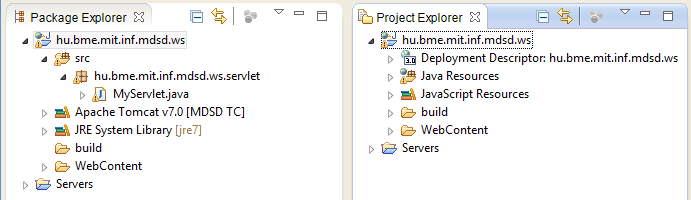
\includegraphics{img/eclipse_basics/package_vs_project_explorer.png}
\caption{The Package Explorer and the Project Explorer in the same
workspace}
\end{figure}

You may want to show the \texttt{.project} file in the \textbf{Package
Explorer}. In order to do so, click the downward pointing triangle in
the upper right corner, pick \textbf{Filters\ldots{}} and untick the
\textbf{.* resources} checkbox.

\begin{figure}[htbp]
\centering
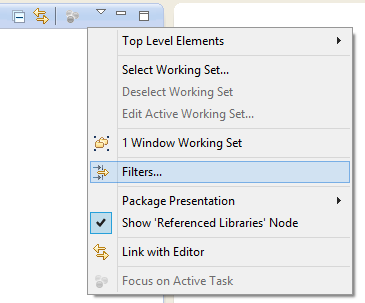
\includegraphics{img/eclipse_basics/package_explorer_filters.png}
\caption{The \textbf{Filters\ldots{}} menu in the \textbf{Package
Explorer}}
\end{figure}

To show the \texttt{.project} file in the \textbf{Project Explorer},
click the downward pointing triangle in the upper right corner, pick
\textbf{Customize View\ldots{}} and untick the \textbf{.* resources}
checkbox.

\subsection{Build in Eclipse}

Eclipse's build philosophy is to always keep the source code and the
binary code in synch. In order to do so, Eclipse builds the project
automatically upon every save operation.

You may turn of the automatic build process by unchecking the
\textbf{Project \textbar{} Build Automatically} menu. However, as a
general rule you should not turn the automatic build off.

\subsection{Copying and linking}

Naturally it is possible to add another file to an existing project. It
can be done by dragging and dropping it to your project. As a result a
dialog window will appear that ask if the file should be copied to the
workspace or just referenced (and left it in its original place).

In addition to the basic file management this operation is useful for
the version control of documents that are edited outside Eclipse. Manual
refresh is required if a file changes out of the IDE.

\subsection{Pictograms}

The \textbf{Package Explorer} and \textbf{Project Explorer} uses a lot
of different icons and pictograms. You can find the description if these
here:
\url{http://help.eclipse.org/juno/index.jsp?topic=/org.eclipse.jdt.doc.user/reference/ref-icons.htm}

\subsection{Subversion}

\textbf{Apache Subversion} (\url{http://subversion.apache.org/}), often
abbreviated SVN is a widely used open-source version control system.

Eclipse does not include an SVN client by default. You can install the
\textbf{Subclipse} plug-in from your Eclipse distribution's
(e.g.~Juno's) update site by following the instructions provided here:
\url{http://www.eclipse.org/subversive/}.

For basic usage you only need the \textbf{Subversive SVN Team Provider}
package. Complete the installation and restart Eclipse. Eclise will ask
you to install a Subversive Connector. Choose one which is compatible
with your SVN server's version, install and restart Eclipse again.

\textbf{Subclipse} pictograms:
\url{http://stackoverflow.com/questions/3917925/what-do-the-arrow-icons-in-subclipse-mean}

\section{User interface}

\subsection{Workbench}

Upon launching, after you choose the workspace location, the workbench
window is shown. A workbench window offers \emph{perspectives}. A
perspective contains editors, such as the Java Editor and views, such as
the Project Explorer.

\subsection{Editors}

Editors contribute buttons to the \emph{global toolbar}. You can have
several instances of the same editor, e.g.~you can have a dozen Java
source files open and edited. You may run different editors at the same
time, e.g.~you can edit Java and XML files in the same workbench.
Editors can be associated with a file name or an extension, and this
association can be changed by users.

\subsection{Views}

The primary use of views is to provide navigation of the information in
the workbench. You can think of a view as a representation of the data
in the workbench. Views have a \emph{local toolbar}. Editors can appear
in only one region of the page, whereas views can be moved to any part
of the page and minimized as fast views.

The default JDT views include the \textbf{Package Explorer}, the
\textbf{Problems}, the \textbf{Console} view and others. You can open
new views in the \textbf{Window \textbar{} Show View} menu.

\subsubsection{The Problems view and the Error Log view}

The \textbf{Problems view} shows the warnings and errors in the
workspace's projects. In the \textbf{Problems} view click on the
Downward pointing triangle icon and pick \textbf{Show \textbar{}
Errors/warnings on selection}.

The \textbf{Error Log} shows the errors occured in Eclipse. It shows the
error message, the date and the plug-in that produced the error.

\begin{figure}[htbp]
\centering
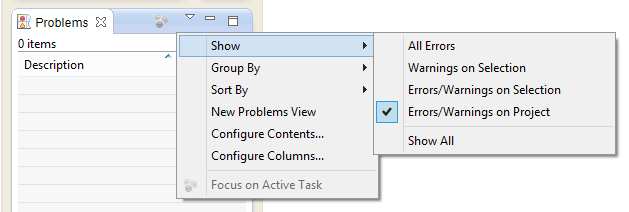
\includegraphics{img/eclipse_basics/problems.png}
\caption{Show error and warning on selection}
\end{figure}

Further reading:

\begin{itemize}
\itemsep1pt\parskip0pt\parsep0pt
\item
  \url{http://wiki.eclipse.org/FAQ_What_is_a_view\%3F}
\item
  \url{http://wiki.eclipse.org/FAQ_What_is_the_difference_between_a_view_and_an_editor\%3F}
\end{itemize}

\subsection{Perspective}

A perspective is a collection and a predefined layout for editors and
views created for a special development purpose: Java, Debug, Plug-in
Development, SVN Repository Exploring, etc.

\subsection{SWT}

Java applications typically use AWT (Abstract Window Toolkit) or the
Swing toolkit to implement graphical user interfaces. While these are
proven solutions, both have serious shortcomings:

\begin{itemize}
\itemsep1pt\parskip0pt\parsep0pt
\item
  AWT uses native widgets, but only provides the ones which are
  available on all supported platforms. Also, AWT's architecture implies
  that the developer has to work on a low level. Hence, AWT is not
  suitable for modern application development.
\item
  Swing provides its own custom widgets and is easily extensible. Swing
  provides the option of using either a system ,,look and feel'' which
  uses the native platform's look and feel, or a cross-platform look and
  feel that looks the same on all windowing-system. The old Swing
  implementation suffered from memory consumption and performance
  problems.
\end{itemize}

SWT (Standard Widget Toolkit) is a GUI framework that was developed for
the Eclipse project by IBM. It uses native components and offers good
performance. Today, SWT is maintained by the Eclipse Foundation. Since
the SWT implementation is different for each platform, a
platform-specific SWT library (JAR file) must be distributed with each
application. A number of SWT widgets are available at
\url{http://eclipse.org/swt/widgets/}.

\begin{figure}[htbp]
\centering
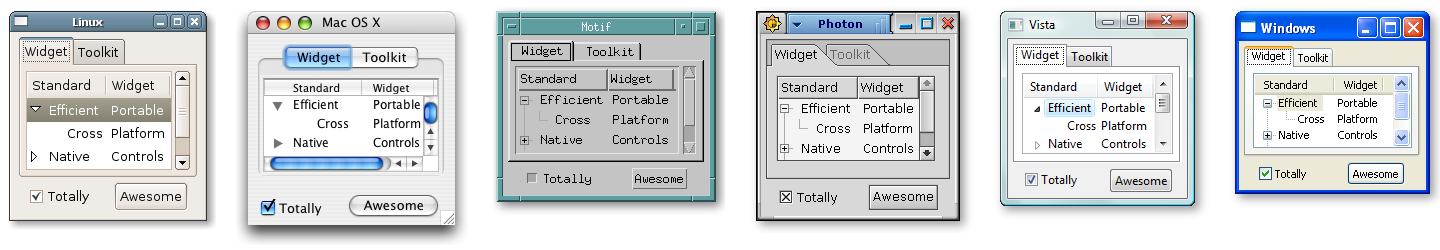
\includegraphics{img/eclipse_basics/swt.png}
\caption{SWT widgets on different platforms}
\end{figure}

\subsection{Search}

\begin{itemize}
\itemsep1pt\parskip0pt\parsep0pt
\item
  Search in files: press \texttt{Ctrl}+\texttt{H} to display the
  \textbf{Search} window and choose the \textbf{File Search} tab. If the
  window has many tabs, the \textbf{File Search} tab may be hidden. The
  solution is to resize the \textbf{Search} window or use the arrows in
  the upper right corner to show the rest of the tabs.
\end{itemize}

\begin{figure}[htbp]
\centering
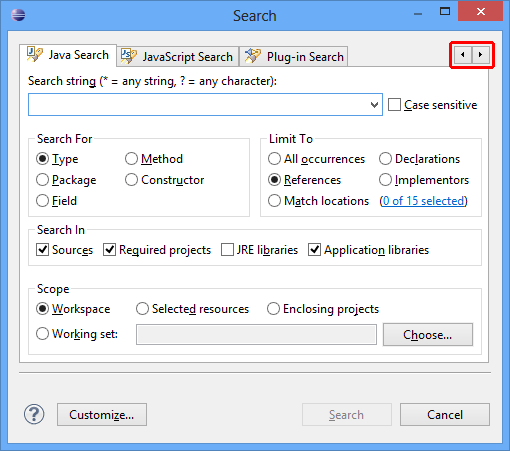
\includegraphics{img/eclipse_basics/search.png}
\caption{The \textbf{File Search} tab may does not appear at first:
resize the window or use the arrows}
\end{figure}

\section{Configuration}

\subsection{Bundle}

OSGi components are named \emph{bundles}. It's important to note that
Eclipse plug-ins are also OSGi bundles.

\subsection{Build path}

If a Java project depends on libraries in JAR files, you have to specify
the JAR files containing those. In order to do so, you have to add the
JAR file to the build path by right clicking on it and picking
\textbf{Build Path \textbar{} Add to Build Path}.

By convention, JAR files are typically stored in a directory called
\texttt{lib}. You cannot add a directory to the build path: you have to
specify the files. If you want to remove a JAR from the build path, you
have to find it under \textbf{Referenced Libraries}, right click and
choose \textbf{Build Path \textbar{} Remove from Build Path}.

If you right click anywhere under the project and choose \textbf{Build
Path \textbar{} Configure Build Path\ldots{}}, you can specify the
source folders and the requires libaries.

\subsection{Execution environment}

In the \textbf{Window \textbar{} Preferences} dialog click \textbf{Java
\textbar{} Installed JREs}. You can add new execution environments and
pick the default one.

\subsection{Run configuration}

Eclipse stores the launch settings in \emph{run configurations}. By
default, run configurations are only saved in the workspace. If you want
to save or share your run configurations, go to the \textbf{Run
Configurations\ldots{}} (under the \textbf{Run} button or right click on
the project and under \textbf{Run As}). On the \textbf{Common} tab
choose \textbf{Shared file} in \textbf{Save as} group.

If you run multiple programs, you can switch between them by clicking
the terminal-shaped icon (called \textbf{Display selected console}).

\subsection{The \texttt{.project} file}

There is a configuration file in every Eclipse project named
\texttt{.project}. To make the \texttt{.project} file visible from
Eclipse, refer to the \emph{Package Explorer and Project Explorer}
section. At first this defines the tool set that works with the project
by naming the natures applied to them. For example the plug-in projects
have the following natures:

\begin{Shaded}
\begin{Highlighting}[]
\KeywordTok{<natures>}
    \KeywordTok{<nature>}\NormalTok{org.eclipse.jdt.core.javanature}\KeywordTok{</nature>}
    \KeywordTok{<nature>}\NormalTok{org.eclipse.pde.PluginNature}\KeywordTok{</nature>}
\KeywordTok{</natures>}
\end{Highlighting}
\end{Shaded}

Secondly it defines the builders that run after every save. In plug-in
projects Eclipse builds the Java code, the \texttt{MANIFEST.MF} and the
\texttt{plugin.xml} with the following configuration:

\begin{Shaded}
\begin{Highlighting}[]
\KeywordTok{<buildSpec>}
  \KeywordTok{<buildCommand>}
    \KeywordTok{<name>}\NormalTok{org.eclipse.jdt.core.javabuilder}\KeywordTok{</name>}
    \KeywordTok{<arguments>}
    \KeywordTok{</arguments>}
  \KeywordTok{</buildCommand>}
  \KeywordTok{<buildCommand>}
    \KeywordTok{<name>}\NormalTok{org.eclipse.pde.ManifestBuilder}\KeywordTok{</name>}
    \KeywordTok{<arguments>}
    \KeywordTok{</arguments>}
  \KeywordTok{</buildCommand>}
  \KeywordTok{<buildCommand>}
    \KeywordTok{<name>}\NormalTok{org.eclipse.pde.SchemaBuilder}\KeywordTok{</name>}
    \KeywordTok{<arguments>}
    \KeywordTok{</arguments>}
  \KeywordTok{</buildCommand>}
\KeywordTok{</buildSpec>}
\end{Highlighting}
\end{Shaded}

\section{The Java source code editor}

Right click the left bar in the source code editor and pick \textbf{Show
Line Numbers}.

\subsection{Formatting the source code}

In a modern IDE you rarely have to format the code by hand. In Eclipse,
right click in the editor and pick \textbf{Source \textbar{} Format}.
Hotkey: \texttt{Ctrl}+\texttt{Shift}+\texttt{F}.

\subsection{Refactoring}

You often need to rename classes, methods and variables. Doing this by
hand is an error-prone method: you may forget to rename some occurences
of the renamed item. The \emph{rename refactoring} technique takes care
of all occurences of the renamed item. To use it, right click on the
renamed item and pick \textbf{Refactor \textbar{} Rename\ldots{}}. Type
the desired name and press \texttt{Enter}. Hotkey:
\texttt{Alt}+\texttt{Shift}+\texttt{R}.

\subsection{Fixing problems}

JDT has a very useful feature called \emph{Quick fix}: if there is an
error or warning in the source code, it suggests common ways of fixing
it (e.g.~if you forgot assign a value to an undefined variable, it will
define it). Hotkey: \texttt{Ctrl}+\texttt{1}.

\subsection{Zooming}

By default, Eclipse does not provide zooming in the editor. You can
change the font size by going to \textbf{Window \textbar{} Preferences}.
Pick \textbf{General \textbar{} Appearance \textbar{} Colors and Fonts},
and edit \textbf{Basic \textbar{} Text Font}.

\subsection{Content assist and imports}

You can access the content assist by pressing
\texttt{Ctrl}+\texttt{Space}. Press \texttt{Enter} to pick you choice.
If you pick an item that has to import a package, the appropriate
\texttt{import} instructinon will appear between the imports. Sometimes
you may end up with lots of unused imports: right click and pick
\textbf{Source \textbar{} Organize Imports} or press
\texttt{Ctrl}+\texttt{Shift}+\texttt{O}.

Pay attention to the package names. For example, the \texttt{List} class
is available both in \texttt{java.awt} and \texttt{java.util}.

\begin{figure}[htbp]
\centering
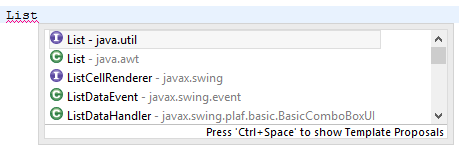
\includegraphics{img/eclipse_basics/content_assist.png}
\caption{Some classes are available in more packages}
\end{figure}

You can use the content assist by only typing the abbreviation of the
desired item. For example, if you have
\texttt{java.io.InputStreamReader} imported, you can type \texttt{ISR}
and the content assist will propose \texttt{InputStreamReader}.

If you want to overwrite an item (class name, method name) with the
content assist, hold the \texttt{Ctrl} button when you press
\texttt{Enter} to pick your choice.

There is a lot of predefined template available in the \textbf{Window
\textbar{} Preferences} dialog under \textbf{Java \textbar{} Editor
\textbar{} Templates}. For example, you can type \texttt{sysout} to get
\texttt{system.out.println();}.

You can use templates for control structures, you can define cycles with
\texttt{for}, \texttt{while}, \texttt{do}, \texttt{foreach} and so on.
Similarly, you can define conditional statement with \texttt{if},
\texttt{ifelse} and \texttt{switch}.

Tip: \textbf{Organize Imports} can also be used to add missing imports.
If the class is available in multiple packages, Eclipse will prompt you
to choose between them.

\subsection{Automatic generation of getter and setter methods}

Since the Java language lacks properties, you often have to write getter
and setter method for the fields you want to access. Fortunately, you
can generate them: right click in the source file and pick
\textbf{Source \textbar{} Generate Getters and Setters\ldots{}}.
Similarly, you can generate the constructor, the \texttt{toString}
method and so on.

If you have only a few properties, there is a quicker way. While typing
\texttt{getVariableName} or \texttt{setVariableName}, use the Content
Assist (\texttt{Ctrl}+\texttt{Space}), pick the desired method and press
\texttt{Enter}. The appropriate method is generated.

\section{Plug-in development}

Multiple pre-compiled editions are available at the home page of Eclipse
(\url{http://www.eclipse.org/downloads/}). One support C/C++
development, an other aids the testing of software. This IDE is not
limited to support those popular field of use; it is designed to be as
customisable as possible. It can be used for example as a LaTeX editor,
as a host of custom enterprise software (e.g.~accounting) or even as a
note sheet editor
(\url{http://mit.bme.hu/~rath/pub/theses/diploma_harmathd.pdf}).

So feel free to look for the tools that support your goals.

If you're interested in the topic, the FTSRG has two related courses to
offer:

\begin{itemize}
\itemsep1pt\parskip0pt\parsep0pt
\item
  Eclipse Technologies: \url{http://www.inf.mit.bme.hu/edu/courses/eat}
\item
  Eclipse Based Development and Integration:
  \url{http://www.inf.mit.bme.hu/edu/courses/eafi}
\end{itemize}

\subsection{Plug-in}

Eclipse's main strength is the possibility of creating and installing
custom Eclipse plug-ins. Some useful ones are:

\begin{itemize}
\itemsep1pt\parskip0pt\parsep0pt
\item
  TeXlipse (\url{http://texlipse.sourceforge.net/}): ,,a plugin that
  adds Latex support to the Eclipse IDE.'' TeXlipse provides incremental
  compiling and easy navigation between the TeX source and the generated
  PDF.
\item
  FindBugs (\url{http://findbugs.sourceforge.net/}): ,,a program which
  uses static analysis to look for bugs in Java code''.
\item
  PMD (\url{http://pmd.sourceforge.net/}): ,,PMD is a source code
  analyzer. It finds unused variables, empty catch blocks, unnecessary
  object creation, and so forth.''
\end{itemize}

FindBugs and PMD are widely used tools. They're also part of the
\emph{Software Verification Techniques} course
(\url{http://www.inf.mit.bme.hu/edu/courses/szet/}) of the ,,Dependable
System Design'' master's programme held in the autumn semester.

\subsection{Runtime Eclipse}

The Eclipse plug-ins run in an Eclipse instance. If new plug-ins are
developed (as Plug-in projects) in an Eclipse instance (called
\textbf{host Eclipse}), there should be an Eclipse instance that can run
them as a part of it in a new empty workspace. This so called
\textbf{runtime Eclipse} contains the plug-ins installed to the host
Eclipse \emph{and} the ones developed in the host Eclipse.

A runtime can be started with the \textbf{Run} button. The range of the
applied plug-ins can be reduced in the run configuration.

It is possible to install developed plug-in projects (see: Install as a
plug-in).

\subsection{RCP}

Eclipse RCP (Rich Client Platform) ,,is a platform for building and
deploying rich client applications. It includes Equinox, a component
framework based on the OSGi standard, the ability to deploy native GUI
applications to a variety of desktop operating systems, such as Windows,
Linux and Mac OSX and an integrated update mechanism for deploying
desktop applications from a central server.''

Along successful open-source projects, RCP is often used for making
highly specialised software for organisations.

Popular RCP applications include the following:

\begin{itemize}
\itemsep1pt\parskip0pt\parsep0pt
\item
  ECUTE
  (\url{http://sourceforge.net/apps/mediawiki/sblim/index.php?title=Ecute}):
  ,,ECUTE stands for Extensible CIM UML Tooling Environment. It is a
  family of tools that support all phases of the development of CIM
  models, CIM providers, and CIM client applications.`' ECUTE is used in
  the BSc specialisation programme ,,Information Technologies'' on the
  Intelligent Systems Surveillance
  (\url{https://www.inf.mit.bme.hu/edu/bsc/irf}) course.
\item
  XMind (\url{http://www.xmind.net/}): a mind mapping software.
\item
  Vuze, formerly known as Azureus (\url{http://www.vuze.com/}): a
  BitTorrent client.
\end{itemize}

In the Model Driven Software Development and Service Integration courses
we use the following RCP applications:

\begin{itemize}
\itemsep1pt\parskip0pt\parsep0pt
\item
  Bonita Open Solution: \url{http://bonitasoft.com/}
\item
  Yakindu: \url{http://statecharts.org/}
\end{itemize}

For more RCP applications, visit the following links:

\begin{itemize}
\itemsep1pt\parskip0pt\parsep0pt
\item
  \url{http://www.eclipse.org/community/rcpos.php}
\item
  \url{http://www.eclipse.org/community/rcpcp.php}
\end{itemize}

The popular UML and BPMN modelling tool, Visual Paradigm can also be
integrated to Eclipse:
\url{http://www.visual-paradigm.com/product/vpuml/provides/ideintegration.jsp}.

Further reading: \url{http://www.eclipse.org/home/categories/rcp.php}.

\subsection{Update site}

Update sites are used to install new features to the Eclipse
application. You can install new applications in the \textbf{Help
\textbar{} Install New Software\ldots{}} menu by selecting the update
site and the installed components.

After the installation completes, it prompts you to restart Eclipse. If
you don't want to restart yet, you can restart Eclipse later by clicking
\textbf{File \textbar{} Restart}.

\subsection{Install as a plug-in}

Tutorial:
\url{http://www.vogella.com/articles/EclipsePlugIn/article.html\#deployplugin_direct}

\subsection{The \texttt{Manifest.MF} file}

The plug-in project contains a folder named \texttt{META-INF}. This
folder has a file named \texttt{MANIFEST.MF} that describes the
relations of the packages of this project with the other packages. In
simple words, it defines which (Java) package is visible as you edit the
source files in this project, and which package you want to make visible
to other projects. The content this file looks like the following:

\begin{itemize}
\item
  Version numbers of the \texttt{MANIFEST.MF}:

\begin{verbatim}
Manifest-Version: 1.0
Bundle-ManifestVersion: 2
\end{verbatim}
\item
  Names and versions. This can be edited at the \textbf{Overview} page
  of the in the \textbf{Plug-in Editor}. An example content:

\begin{verbatim}
Bundle-ManifestVersion: 2
Bundle-Name: JPADataCompileButton
Bundle-SymbolicName: hu.bme.mit.mdsd.generatebutton;singleton:=true
Bundle-Version: 1.0.0.qualifier
\end{verbatim}
\item
  Required target platform that can run this bundle:

\begin{verbatim}
Bundle-RequiredExecutionEnvironment: JavaSE-1.6
\end{verbatim}
\item
  After this, the configuration file enumerates the required bundles
  with optional minimal version requirement. This can be edited in the
  \textbf{Dependencies} page of the \textbf{Plug-in Editor}. An example:

\begin{verbatim}
Require-Bundle: org.eclipse.ui,
 hu.bme.mit.mdsd.erdiagram;bundle-version="1.0.0",
 hu.bme.mit.mdsd.codegenerator;bundle-version="1.0.0",
 org.eclipse.core.runtime;bundle-version="3.8.0"
\end{verbatim}
\item
  The following section declares the exported packages. This can be
  edited at the \textbf{Runtime} page of the Plug-in editor.

\begin{verbatim}
Export-Package: ERDiagram,
 ERDiagram.impl,
 ERDiagram.util
\end{verbatim}
\end{itemize}

\subsection{The \texttt{plugin.xml} file}

An eclipse plug-in is an OSGi bundle that (usually) connects to other
bundles through an extension point mechanism. An \textbf{extension
point} defines the interface and an \textbf{extension} defines a
subscription to that arbitrary interface. The \texttt{plugin.xml}
configuration file contains those information. This configuration can be
edited in the \textbf{Extension} page of the plug-in editor.

An example subscription that handles a GUI event:

\begin{Shaded}
\begin{Highlighting}[]
\CommentTok{<!-- This is an extension of "org.eclipse.ui.handlers". -->}
\KeywordTok{<extension}
\OtherTok{   point=}\StringTok{"org.eclipse.ui.handlers"}\KeywordTok{>}
   \CommentTok{<!-- If a command named "hu.bme.mit.JPADataCompileButton.GenerateCommand"}
\CommentTok{      fires then call the execute method of the class named}
\CommentTok{      "hu.bme.mit.JPADataCompileButton.GenerateCommand".-->}
   \KeywordTok{<handler}
\OtherTok{      class=}\StringTok{"hu.bme.mit.compilecommandhandler.JPADataGenerateCommandHandler"}
\OtherTok{      commandId=}\StringTok{"hu.bme.mit.JPADataCompileButton.GenerateCommand"}\KeywordTok{>}
   \KeywordTok{</handler>}
\KeywordTok{</extension>}
\end{Highlighting}
\end{Shaded}

\section{Hotkeys}

As every modern IDE, Eclipse defines a great number of hotkeys. We
gathered some useful ones here:

\begin{itemize}
\itemsep1pt\parskip0pt\parsep0pt
\item
  List the available hotkeys: \texttt{Ctrl}+\texttt{Shift}+\texttt{L}.
\item
  Quick fix: \texttt{Ctrl}+\texttt{1}
\item
  Content assist: \texttt{Ctrl}+\texttt{Space}
\item
  Organize imports: \texttt{Ctrl}+\texttt{Shift}+\texttt{O}
\item
  Autoformatting of source code: \texttt{Ctrl}+\texttt{Shift}+\texttt{F}
\item
  Run: \texttt{Ctrl}+\texttt{F11}
\item
  Navigate between tabs: \texttt{Ctrl}+\texttt{Page Up},
  \texttt{Ctrl}+\texttt{Page Down}
\item
  Rename refactoring: \texttt{Alt}+\texttt{Shift}+\texttt{R}
\item
  Find/Replace: \texttt{Ctrl}+\texttt{F}, use \texttt{Ctrl}+\texttt{K}
  to iterate through the results.
\item
  Seach: \texttt{Ctrl}+\texttt{H}
\end{itemize}

You can edit the hotkeys in the \textbf{Window \textbar{} Preferences}
menu, in \textbf{General \textbar{} Keys}. For some plug-ins
(e.g.~TeXlipse), the hotkeys don't appear at first: click the
\textbf{Filters\ldots{}} button and untick the \textbf{Filter
uncategorized commands} checkbox.

\section{Sources}

\begin{itemize}
\itemsep1pt\parskip0pt\parsep0pt
\item
  Our own experience from Project Laboratories, etc.
\item
  University courses: Eclipse Technologies
  (\url{http://www.inf.mit.bme.hu/edu/courses/eat}), Eclipse Based
  Development and Integration
  (\url{http://www.inf.mit.bme.hu/edu/courses/eafi}), Model Driven
  Software Development
  (\url{http://www.inf.mit.bme.hu/edu/courses/mdsd}), Service
  Integration (\url{http://www.inf.mit.bme.hu/edu/courses/szolgint})
\item
  \url{http://www.eclipse.org/documentation/}
\item
  \url{http://theshyam.com/2009/07/eclipse-productivity-shortcuts/}
\item
  \url{http://www.openlogic.com/wazi/bid/221090/Eclipse-productivity-tips}
\item
  \url{http://rithus.com/eclipse-productivity-tips}
\end{itemize}

\chapter{Eclipse laboratory: step-by-step instructions}

\section{Introduction}

We will demonstrate Eclipse on a simple task. We create a Java project
and then extend it to a plug-in project. After that, we import a plug-in
project which puts a button on the Eclipse toolbar and configure it to
print the output of our own plug-in project.

\section{Java project}

Go to \textbf{File \textbar{} New \textbar{} Other\ldots{}}. Here you
can choose any type of projects your Eclipse supports. For now, create
\textbf{Java Project}.

\begin{enumerate}
\def\labelenumi{\arabic{enumi}.}
\item
  Name to project to \texttt{hu.bme.mit.inf.carhandler} and click
  \textbf{Finish}.
\item
  Right click on the project name and choose \textbf{New \textbar{}
  Package}. Name the package to \texttt{hu.bme.mit.inf.cars}.
\item
  Right click the package and choose \textbf{New \textbar{} Class}. Name
  the class to \texttt{Car}.

\begin{Shaded}
\begin{Highlighting}[]
\KeywordTok{public} \KeywordTok{class} \NormalTok{Car \{}
     \KeywordTok{private} \NormalTok{String numberplate;}
     \KeywordTok{private} \DataTypeTok{int} \NormalTok{yearOfManufacture;}
     \KeywordTok{private} \DataTypeTok{double} \NormalTok{acceleration;}
\NormalTok{\}}
\end{Highlighting}
\end{Shaded}

  Right click and go to the \textbf{Source} menu. You can access
  formatting, refactoring and generation tools here. Use the following:

  \begin{itemize}
  \itemsep1pt\parskip0pt\parsep0pt
  \item
    \textbf{Generate Constructor using Fields\ldots{}}
  \item
    \textbf{Generate Getters and Setters\ldots{}}
  \item
    \textbf{Generate toString\ldots{}}
  \item
    \textbf{Format}
  \end{itemize}
\item
  Create a new class named \texttt{CarFleetPrinter}. This time, tick
  \texttt{public static void main(String{[}{]} args)} checkbox so the
  main function is generated automatically. You can create the main
  method later as well, using the \texttt{main} template and content
  assist (\texttt{Ctrl}+\texttt{Space}).

  Write the following code. Hint:

  \begin{itemize}
  \itemsep1pt\parskip0pt\parsep0pt
  \item
    Type \texttt{/**} and press \texttt{Enter} to Javadoc.
  \item
    Use \texttt{Ctrl}+\texttt{1} to use the appropriate package to
    import.
  \item
    Use the content assist to suggest a default name (\texttt{car}) for
    the collection.
  \item
    Type \texttt{LL} and use the content assist to find the
    \texttt{LinkedList} class.
  \item
    Use the \texttt{foreach} and the \texttt{sysout} templates.
  \end{itemize}

\begin{Shaded}
\begin{Highlighting}[]
\CommentTok{/**}
\CommentTok{  * Car dealer program. }
\CommentTok{  * }\KeywordTok{@param args }\CommentTok{Arguments}
\CommentTok{  */}
\KeywordTok{public} \DataTypeTok{static} \DataTypeTok{void} \FunctionTok{main}\NormalTok{(String[] args) \{}
  \NormalTok{String manifest = }\StringTok{"The car fleet consists of:}\CharTok{\textbackslash{}n}\StringTok{"}\NormalTok{;}

  \NormalTok{List<Car> cars = }\KeywordTok{new} \NormalTok{LinkedList<Car>();}
  \NormalTok{Random random = }\KeywordTok{new} \NormalTok{Random();}
  \KeywordTok{for} \NormalTok{(}\DataTypeTok{int} \NormalTok{i = }\DecValTok{0}\NormalTok{; i < }\DecValTok{10}\NormalTok{; i++)}
    \NormalTok{cars.}\FunctionTok{add}\NormalTok{(}
      \KeywordTok{new} \FunctionTok{Car}\NormalTok{(}
        \StringTok{"MIT-"} \NormalTok{+ random.}\FunctionTok{nextInt}\NormalTok{(}\DecValTok{10}\NormalTok{) + random.}\FunctionTok{nextInt}\NormalTok{(}\DecValTok{10}\NormalTok{) + random.}\FunctionTok{nextInt}\NormalTok{(}\DecValTok{10}\NormalTok{), }
        \DecValTok{2000} \NormalTok{+ random.}\FunctionTok{nextInt}\NormalTok{(}\DecValTok{13}\NormalTok{),}
        \FloatTok{3.0} \NormalTok{+ random.}\FunctionTok{nextDouble}\NormalTok{() * }\DecValTok{4}
      \NormalTok{)}
    \NormalTok{);}

  \KeywordTok{for} \NormalTok{(Car car : cars) \{}
    \KeywordTok{if} \NormalTok{(car.}\FunctionTok{getAcceleration}\NormalTok{() < }\DecValTok{5}\NormalTok{) \{}
      \NormalTok{manifest += }\StringTok{"- Car: "} \NormalTok{+ car + }\StringTok{"}\CharTok{\textbackslash{}n}\StringTok{"}\NormalTok{;}
    \NormalTok{\}}
  \NormalTok{\}}

  \NormalTok{System.}\FunctionTok{out}\NormalTok{.}\FunctionTok{println}\NormalTok{(manifest);}
\NormalTok{\}}
\end{Highlighting}
\end{Shaded}
\item
  Use the \textbf{Rename} refactoring technique to rename the class from
  \texttt{Car} to \texttt{SportsCar}.
\item
  Select the following part:

\begin{Shaded}
\begin{Highlighting}[]
\KeywordTok{new} \FunctionTok{Car}\NormalTok{(}
  \StringTok{"MIT-"} \NormalTok{+ random.}\FunctionTok{nextInt}\NormalTok{(}\DecValTok{10}\NormalTok{) + random.}\FunctionTok{nextInt}\NormalTok{(}\DecValTok{10}\NormalTok{) + random.}\FunctionTok{nextInt}\NormalTok{(}\DecValTok{10}\NormalTok{), }
  \DecValTok{2000} \NormalTok{+ random.}\FunctionTok{nextInt}\NormalTok{(}\DecValTok{13}\NormalTok{),}
  \FloatTok{3.0} \NormalTok{+ random.}\FunctionTok{nextDouble}\NormalTok{() * }\DecValTok{4}
\NormalTok{)}
\end{Highlighting}
\end{Shaded}

  Use the \textbf{Extract method} refactoring technique to extract it to
  a method named \texttt{generateRandomCar}.
\item
  Select the whole \texttt{main} method except the last line
  (\texttt{System.out.println(manifest)}). Use the \textbf{Extract
  method} technique again to extract it to a method named
  \texttt{getCarManifest}.
\item
  The result looks like this:

\begin{Shaded}
\begin{Highlighting}[]
\KeywordTok{public} \DataTypeTok{static} \DataTypeTok{void} \FunctionTok{main}\NormalTok{(String[] args) \{}
  \NormalTok{String manifest = }\FunctionTok{getCarManifest}\NormalTok{();}

  \NormalTok{System.}\FunctionTok{out}\NormalTok{.}\FunctionTok{println}\NormalTok{(manifest);}
\NormalTok{\}}

\KeywordTok{private} \DataTypeTok{static} \NormalTok{String }\FunctionTok{getCarManifest}\NormalTok{() \{}
  \NormalTok{String manifest = }\StringTok{"The car fleet consists of:}\CharTok{\textbackslash{}n}\StringTok{"}\NormalTok{;}

  \NormalTok{List<Car> cars = }\KeywordTok{new} \NormalTok{LinkedList<Car>();}
  \NormalTok{Random random = }\KeywordTok{new} \NormalTok{Random();}
  \KeywordTok{for} \NormalTok{(}\DataTypeTok{int} \NormalTok{i = }\DecValTok{0}\NormalTok{; i < }\DecValTok{10}\NormalTok{; i++)}
    \NormalTok{cars.}\FunctionTok{add}\NormalTok{(}
      \FunctionTok{generateRandomCar}\NormalTok{(random)}
    \NormalTok{);}

  \KeywordTok{for} \NormalTok{(Car car : cars) \{}
    \KeywordTok{if} \NormalTok{(car.}\FunctionTok{acceleration} \NormalTok{< }\DecValTok{5}\NormalTok{) \{}
      \NormalTok{manifest += }\StringTok{"- Car: "} \NormalTok{+ car + }\StringTok{"}\CharTok{\textbackslash{}n}\StringTok{"}\NormalTok{;}
    \NormalTok{\}}
  \NormalTok{\}}
  \KeywordTok{return} \NormalTok{manifest;}
\NormalTok{\}}

\KeywordTok{private} \DataTypeTok{static} \NormalTok{Car }\FunctionTok{generateRandomCar}\NormalTok{(Random random) \{}
  \KeywordTok{return} \KeywordTok{new} \FunctionTok{Car}\NormalTok{(}
    \StringTok{"MIT-"} \NormalTok{+ random.}\FunctionTok{nextInt}\NormalTok{(}\DecValTok{10}\NormalTok{) + }
         \NormalTok{random.}\FunctionTok{nextInt}\NormalTok{(}\DecValTok{10}\NormalTok{) + }
         \NormalTok{random.}\FunctionTok{nextInt}\NormalTok{(}\DecValTok{10}\NormalTok{), }
    \DecValTok{2000} \NormalTok{+ random.}\FunctionTok{nextInt}\NormalTok{(}\DecValTok{13}\NormalTok{),}
    \FloatTok{3.0} \NormalTok{+ random.}\FunctionTok{nextDouble}\NormalTok{() * }\DecValTok{4}
  \NormalTok{);}
\NormalTok{\}}
\end{Highlighting}
\end{Shaded}
\item
  To run the project, right click and pick \textbf{Run As \textbar{}
  Java Application}.
\end{enumerate}

\section{Plug-in project}

\begin{enumerate}
\def\labelenumi{\arabic{enumi}.}
\item
  Import the \texttt{hu.bme.mit.inf.car.carbutton} project from the
  \texttt{CarButton.zip} file. Use the \textbf{File \textbar{} Import}
  menu and choose \textbf{General \textbar{} Existing Projects into
  Workspace} and use the \textbf{Select archive file} option.
\item
  Inspect the \texttt{plugin.xml} and \texttt{META-INF/MANIFEST.MF}
  file. The most interesting for now are the \textbf{Extensions} tab.
\item
  Run the project by right clicking the project and picking \textbf{Run
  As \textbar{} Eclipse Application}. A new Eclipse instance called
  ,,Runtime Eclipse'' will start with the plug-in. Close the welcome
  Window. Observe the \textbf{Print!} button on the toolbar.
\item
  Close the Runtime Eclipse.
\item
  We would like to extend our Java project to a plug-in project. Right
  click the \texttt{hu.bme.mit.inf.carhandler} project and choose
  \textbf{Configure \textbar{} Convert to Plug-in Projects\ldots{}}.
  Click \textbf{Finish}.
\item
  Go to the \texttt{carhandler} project's newly created
  \texttt{MANIFEST.MF} file. Pick the \textbf{Runtime} tab. Observe the
  \textbf{Exported Packages}. Later, you can add additional packages if
  necessary.
\item
  Go to the \texttt{carbutton} project's \texttt{MANIFEST.MF} file. Pick
  the \textbf{Dependencies} tab.
\item
  Click \textbf{Add}. An empty list will show. However, as soon as you
  start typing \texttt{car}, the
  \texttt{hu.bme.mit.inf.carhandle (1.0.0.qualifier)} package will show.
  Click \textbf{OK}.
\item
  Go to the \texttt{hu.bme.mit.inf.car.carbutton} package's
  \texttt{PrintTheCarHandler} file. Inspect the \texttt{showMessage}
  method which shows a message in a dialog window.
\item
  In the \texttt{execute} method use \texttt{showMessage} to show the
  car fleet's data.

\begin{Shaded}
\begin{Highlighting}[]
\FunctionTok{showMessage}\NormalTok{(CarFleetPrinter.}\FunctionTok{getCarManifest}\NormalTok{());}
\end{Highlighting}
\end{Shaded}

  Use \textbf{Quick Fix} take care of the missing
  \texttt{CarFleetPrinter} import and change the visibility of the
  method.
\item
  Run the plug-in project. This time, the \textbf{Print!} button will
  show the cars in the fleet.
\end{enumerate}

\begin{figure}[htbp]
\centering
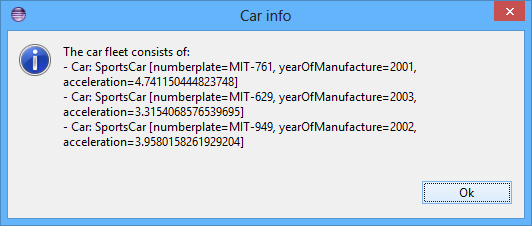
\includegraphics{img/eclipse_basics/message.png}
\caption{The message shown in the plug-in project.}
\end{figure}

\section{Version control}

From the \textbf{Window \textbar{} Open Perspective \textbar{}
Other\ldots{}} pick the \textbf{SVN Repository Exploring} perspective.
Use the green plus icon (\textbf{New Repository Location}) to add a new
repository. (You can also import from the \textbf{File \textbar{}
Import} menu with the \textbf{SVN \textbar{} Project from SVN} option.)
\& Specify the URL and fill the authentication data appropriately. If
you're working on a private computer, it's recommended to save the
authentication data.

Click \textbf{Finish}. For now, don't bother with the password recovery
feature.

\subsection{Sharing projects}

If you have configured a Subversion repository, you can easily share
your projects. Right click on the project name and pick \textbf{Team
\textbar{} Share Project\ldots{}}.

Choose \textbf{SVN} and choose your repository location and specify the
target URL. Pay attention to always include the project name as the last
directory in the path. (Warning: if you use the \textbf{Browse\ldots{}}
button, it will not be added automatically).

Click \textbf{Finish}. In the \textbf{Commit} window fill the commit
message and click \textbf{OK}.

If you ever decide to stop using version control for a project
(e.g.~your version tracking got messed up), go to right click menu and
choose \textbf{Team \textbar{} Disconnect}. When Eclipse prompts you to
confirm the question, choose the \textbf{Also delete the SVN
meta-information from the file system.} which deletes the hidden
\texttt{.svn} directories.

\begin{figure}[htbp]
\centering
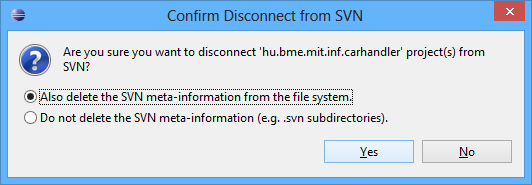
\includegraphics{img/eclipse_basics/svn_disconnect.png}
\caption{Use the first option when disconnecting from SVN.}
\end{figure}

You can commit files by choosing \textbf{Team \textbar{}
Commit\ldots{}}, update files by \textbf{Update}. You can also make good
use of the \textbf{Revert} and \textbf{Revert to commit} options.

If more than one person works on a file, a conflict can emerge.

\begin{figure}[htbp]
\centering
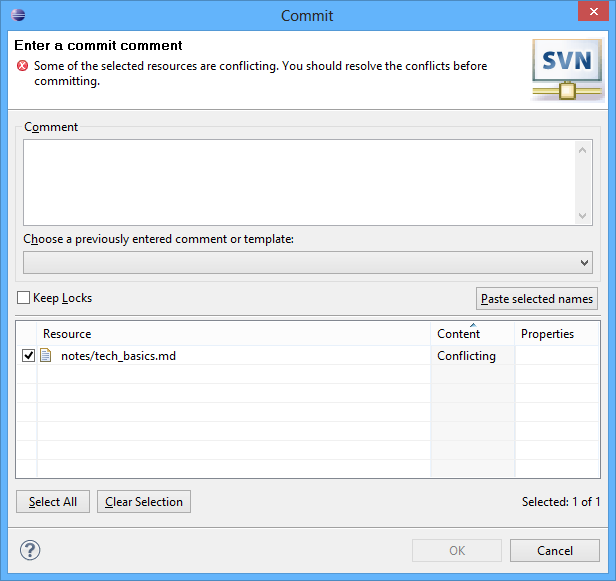
\includegraphics{img/eclipse_basics/svn_commit_conflict.png}
\caption{Conflicting resources}
\end{figure}

To resolve the conflict, use the \textbf{Team Synchonizing} perspective
or right click on the file and choose \textbf{Team \textbar{} Edit
Conflicts}.

\begin{figure}[htbp]
\centering
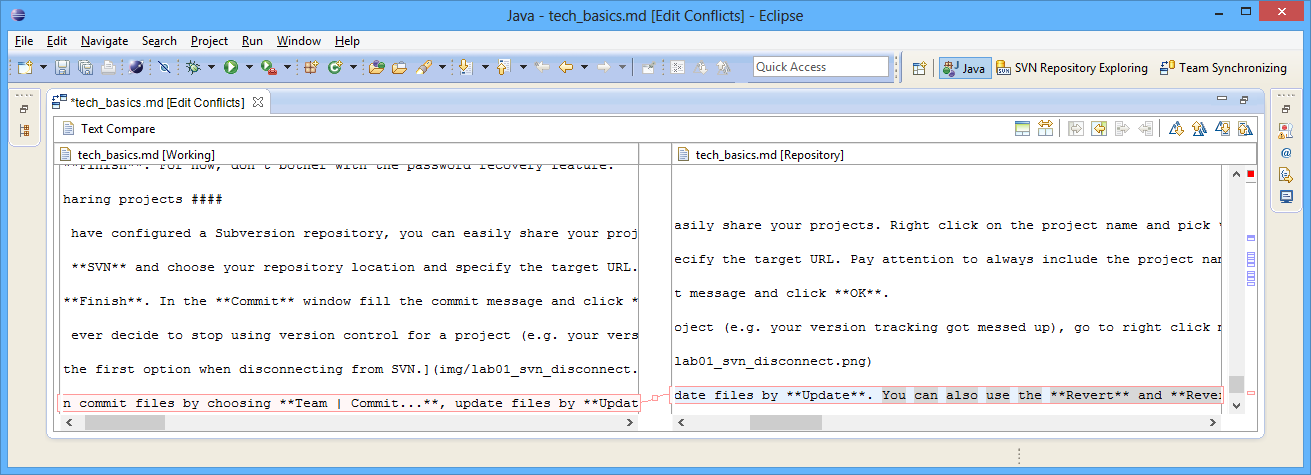
\includegraphics{img/eclipse_basics/svn_conflict_resolve.png}
\caption{Resolving the conflict in the \textbf{Team Synchronizing}
perspective.}
\end{figure}

Further reading:
\url{http://help.eclipse.org/juno/index.jsp?topic=/org.eclipse.platform.doc.user/tasks/tasks-115.htm}

\chapter{BPMN}

\section{Introduction}

BPMN (Business Process Model and Notation) is a widely used graphical
representation for specifying business processes in a business process
modell.

On the Service Integration course, we will use Bonita as our BPMN editor
and workflow framework. Bonita is an Eclipse RCP application.

\begin{figure}[htbp]
\centering

\includegraphics{img/bpmn/bonita_logo.png}
\caption{The logo of BonitaSoft}
\end{figure}

\section{Sources}

\begin{itemize}
\itemsep1pt\parskip0pt\parsep0pt
\item
  \url{http://www.bonitasoft.com/}
\item
  \url{http://www.bpmn.org/}
\end{itemize}

\chapter{BPMN laboratory -- step-by-step instructions}

In this laboratory, we will create the workflow of an application store.
In the application store the users can browse and upload applications.
On the Model Driven Software Development and Service Integration Courses
In 2012, the teams had to design and implement the workflow of an
application store.

\section{Simple workflow}

\begin{enumerate}
\def\labelenumi{\arabic{enumi}.}
\item
  Start \textbf{Bonita Studio}. Bonita will prompt you to register. You
  can choose to skip it but it's highly recommended to register because
  registration provides access to well-made official tutorials and
  thorough documentation.

  \begin{figure}[htbp]
  \centering
  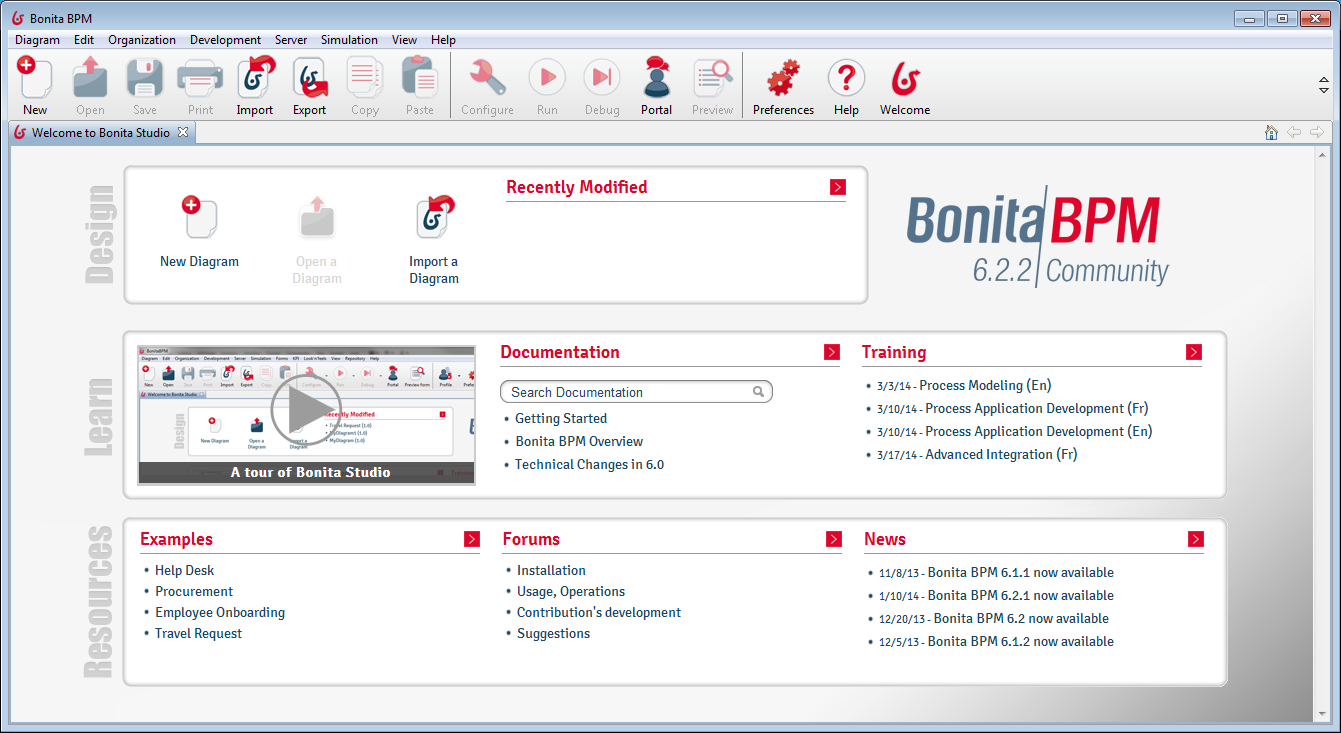
\includegraphics{img/bpmn/bonita_opening.png}
  \caption{The opening screen of Bonita}
  \end{figure}
\item
  Create a new process from \textbf{Process \textbar{} New}.
\item
  A simple process will show with only a \emph{start event} and a
  \emph{human task}. Click on the process, choose the \textbf{Pool} page
  and click the \textbf{Edit\ldots{}}* button. Rename the process to
  \texttt{Browse Application}.
\item
  Click the \texttt{Step1} task and look at it's properties on the
  \textbf{General} tab. On this tab, you can set the execution-specific
  properties of the process, e.g.~it's \textbf{Name} and \textbf{Task
  type}. Rename the task to \texttt{Acknowledge}.
\item
  Add an \emph{end event} to the workflow. Connect the
  \texttt{Acknowledge} to the end event.

  \begin{figure}[htbp]
  \centering
  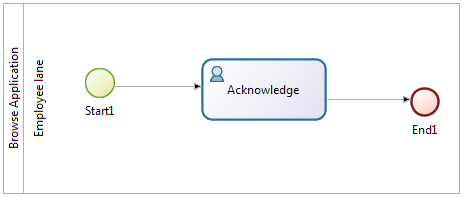
\includegraphics{img/bpmn/bonita_hello_task_editor.png}
  \caption{The \texttt{Browse Application} process}
  \end{figure}
\item
  Let's create a graphical user interface for this task. Choose the
  \textbf{Application} tab. On the \textbf{Entry Pageflow} page click
  \textbf{Add\ldots{}}. Click \textbf{Finish}.
\item
  A graphical editor will appear. Add a \textbf{message} to the top of
  the form. Edit the properties of the message element on the
  \textbf{Data} page. You can edit plain text or HTML code. Type
  \texttt{Hello world!}.
\item
  Click the \textbf{Run} button or choose your process in the
  \textbf{Run \textbar{} Run} menu. The generated web page will show in
  a browser.

  \begin{figure}[htbp]
  \centering
  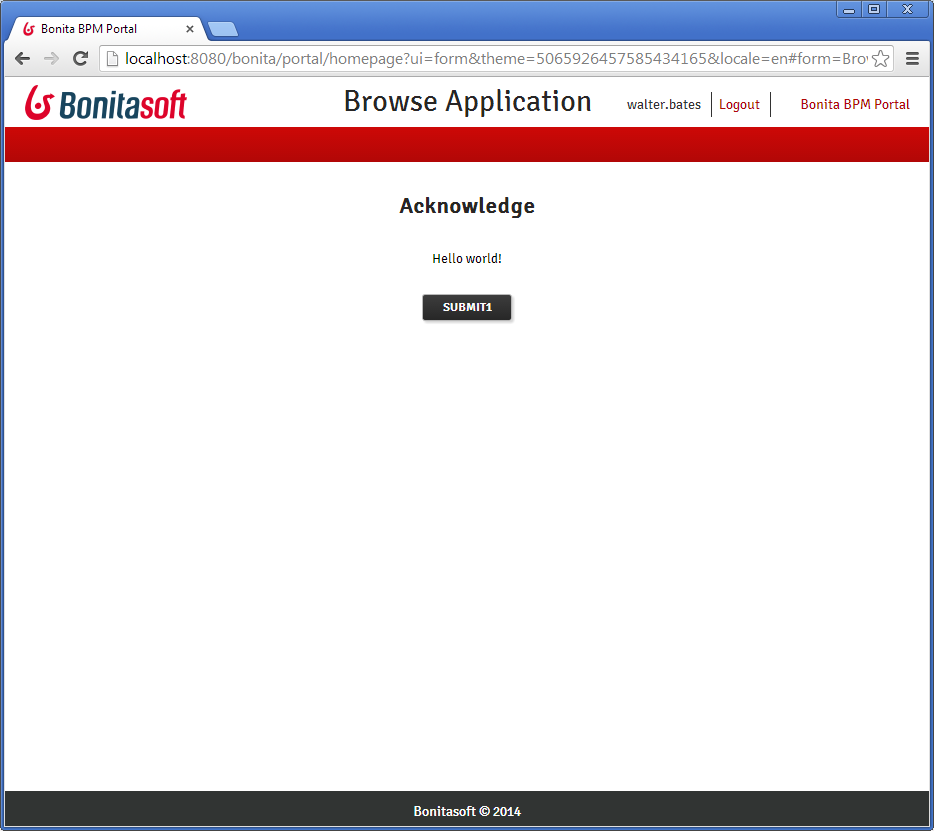
\includegraphics{img/bpmn/bonita_hello_task_browser.png}
  \caption{The \texttt{Hello task} in the browser}
  \end{figure}
\item
  On the web interface, you can control the workflow by the buttons
  provided. In this example, if you click the \textbf{Submit1} button,
  the workflow finishes.
\item
  Click to the UserXP button and browse this interface. Try to start a
  new workflow from this.
\item
  Create the following tasks:

  \begin{itemize}
  \itemsep1pt\parskip0pt\parsep0pt
  \item
    \texttt{Download the application names}: \emph{abstract task}.
  \item
    \texttt{Show the applications}: \emph{human task}.
  \item
    \texttt{Buy the application}: \emph{abstract task}.
  \end{itemize}
\item
  The \texttt{Show the applications} human task is not associated with
  an actor. Click the task and choose the \textbf{Actors} page. Next to
  the \textbf{Actor Selectors} box, click the \textbf{Choose\ldots{}}
  button and select the \textbf{Initiator}. The \textbf{Initiator} is
  the role of the person who starts the task.

  \begin{figure}[htbp]
  \centering
  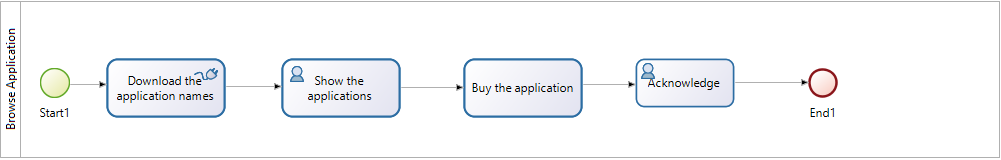
\includegraphics{img/bpmn/bonita_browse_application_process.png}
  \caption{The \texttt{Browse Application} process}
  \end{figure}
\item
  Let's add some workflow variables to the process. Click the process
  and choose the \textbf{Data} page. Create the following variables:

  \begin{itemize}
  \itemsep1pt\parskip0pt\parsep0pt
  \item
    \texttt{Applications}: is the collection of names of the
    downloadable applications. The type of this variable is
    \texttt{Text} and the multiplicity is \texttt{Multiple}.
  \item
    \texttt{SelectedApplication}: The user will select one of the
    available application. This \texttt{Text} variable with
    \texttt{Single} multiplicity contains the name of it.
  \end{itemize}

  \begin{figure}[htbp]
  \centering
  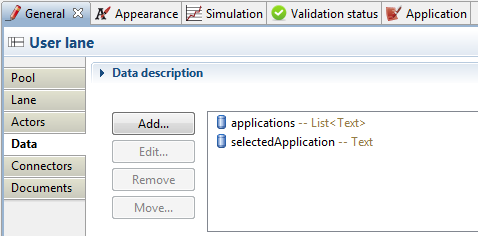
\includegraphics{img/bpmn/bonita_process_data.png}
  \caption{The variables of the \texttt{Browse Application} process}
  \end{figure}
\item
  Let's create a script that substitutes the calling of other services.
  Select the \textbf{Download the application names} task and go to the
  \textbf{Connectors} page. Add a new script by selecting
  \textbf{Scripting \textbar{} Groovy -- Execute a Groovy script}.
\item
  Name the script instance to \textbf{Get the applications}, time it to
  the enter of the activity and hit next. At this window select the
  \textbf{Edit expression\ldots{}} option from the combobox, and a
  conviniant Groovy editor will apear to write our script in it. This
  allows us to edit a Java-like expression or a method body where every
  flow variable is available.

  \begin{figure}[htbp]
  \centering
  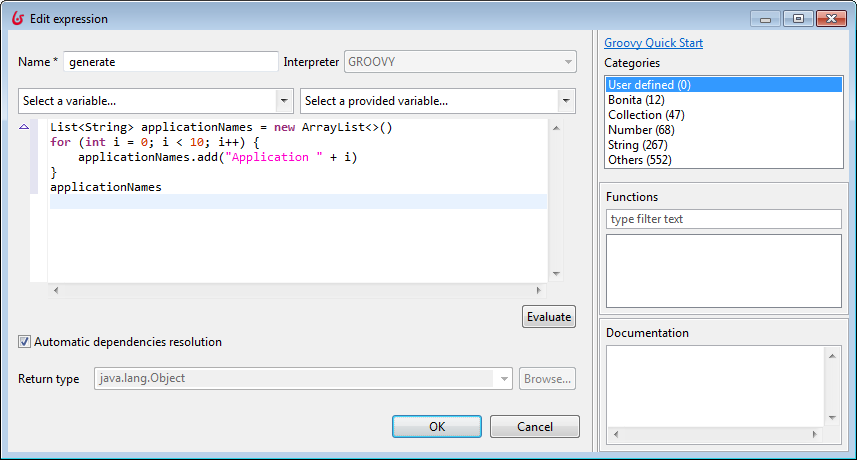
\includegraphics{img/bpmn/bonita_groovy_editor.png}
  \caption{The Groovy editor}
  \end{figure}
\item
  Create this script that returns a collection of application name:

\begin{Shaded}
\begin{Highlighting}[]
\NormalTok{List<String> applicationNames = }\KeywordTok{new} \NormalTok{LinkedList<String>()}
\KeywordTok{for} \NormalTok{(}\DataTypeTok{int} \NormalTok{i = }\DecValTok{0}\NormalTok{; i < }\DecValTok{10}\NormalTok{; i++) \{}
  \NormalTok{applicationNames.}\FunctionTok{add}\NormalTok{(}\StringTok{"Application "} \NormalTok{+ i)}
\NormalTok{\}}
\KeywordTok{return} \NormalTok{applicationNames}
\end{Highlighting}
\end{Shaded}

  Click next and direct the result of this script to the
  \texttt{applications} variable and choose the \textbf{REPLACE}
  strategy.
\item
  Add a graphical view to the \textbf{Show the applications} task. There
  will be a section named \textbf{All widget based on\ldots{}} that
  automatically derives the view from the checked flow variables. In
  this case we want to specify every element so unselect all.

  Drag a \textbf{Radio buttons} widget to the top of the view ad go to
  the data page of the property view. We would like to show the
  application names in this list, so got to the \textbf{Avaible values}
  and select the \textbf{\$\{applications\}\ldots{}} option from the
  right side. As you select it a window should appear where you pick the
  ``The whole list of values'' option.

  We also want to put the name of the selected value to a variable, so
  edit that the \texttt{\$\{field\_Radio\_buttons1\}} saves to
  \textbf{selectedApplication}.

  \begin{figure}[htbp]
  \centering
  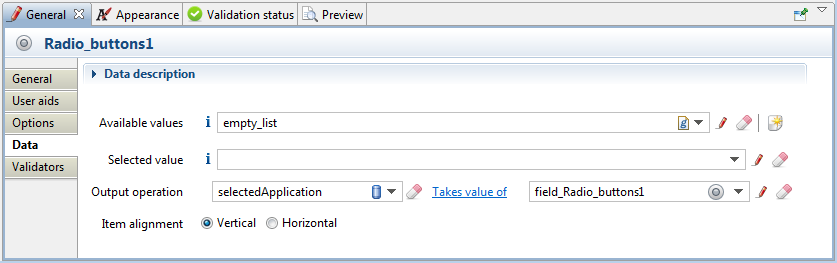
\includegraphics{img/bpmn/bonita_radio_buttons.png}
  \caption{The final properties of the radiobuttons.}
  \end{figure}
\item
  The message of the \textbf{Acknowledge} action should refer to the
  selected variable, so let's set it. If you closed the editor page go
  to the properties of the action select the \textbf{Application} page
  and edit the \textbf{Hello task} pageflow.

  At the \textbf{Data} page \texttt{Hello world!} message with an
  expression by the \textbf{Edit expression\ldots{}} option and write
  that:

\begin{Shaded}
\begin{Highlighting}[]
\StringTok{"Thank you for downloading the "} \NormalTok{+ selectedApplication + }\StringTok{" application."}
\end{Highlighting}
\end{Shaded}
\item
  Try to run the application. Don't be afraid of the presettable
  variable at the begining.
\item
  Sone time an action may fail and the error should be handled. Add a
  script connector \textbf{Buy the application} action. Select the
  \textbf{Throw error event} at the \textbf{If connector fails\ldots{}}
  options and name the error ot ``failed''. The script should looks like
  this:

\begin{Shaded}
\begin{Highlighting}[]
\KeywordTok{if}\NormalTok{(selectedApplication == applications.}\FunctionTok{get}\NormalTok{(}\DecValTok{0}\NormalTok{))}
  \KeywordTok{throw} \KeywordTok{new} \NormalTok{UnsupportedOperationException()}
\end{Highlighting}
\end{Shaded}

  This script will fail with an exception if the user downloads the
  first application. The output should be neglected.
\item
  Add a \textbf{Catch error} item to the \textbf{Buy the application}
  action from the palette. Create a human task for the initiator and
  edit the control flow:

  \begin{figure}[htbp]
  \centering
  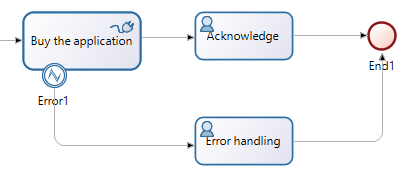
\includegraphics{img/bpmn/bonita_error_handling.png}
  \caption{Error handling flow}
  \end{figure}

  Create a webpage for the task where there is a message that shows
  ``Error in the web services!''.
\item
  Run the workflow and select the first application. It looks like that
  the workflow stops but eventually the next action arrives to the
  inbox.
\end{enumerate}

\begin{figure}[htbp]
\centering
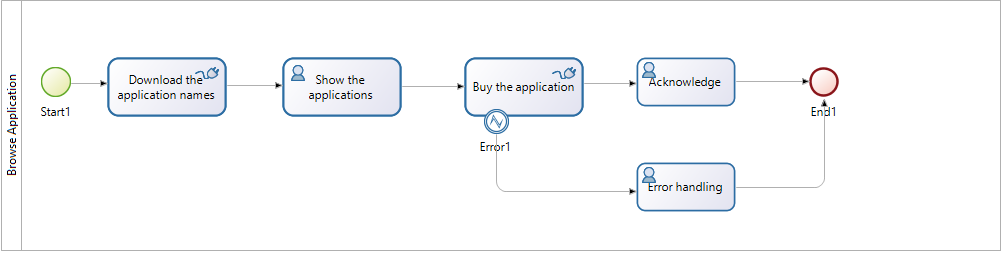
\includegraphics{img/bpmn/bonita_browse_application_process_exceptions.png}
\caption{The final process with exception handling}
\end{figure}

\section{Complex workflow}

We will implement a workflow for the actions of the user.

\begin{enumerate}
\def\labelenumi{\arabic{enumi}.}
\item
  Create a new \emph{pool} and name it to \texttt{User workflow}.
\item
  Create a \emph{start event}, an \emph{end event} and create the
  following tasks:

  \begin{itemize}
  \itemsep1pt\parskip0pt\parsep0pt
  \item
    \texttt{Authenticate}: \emph{service task}
  \item
    \texttt{User action}: \emph{human task}
  \item
    \texttt{Login failed}: \emph{human task}
  \item
    \texttt{Browse applications}: \emph{call activity}
  \item
    \texttt{Upload application}: \emph{abstract task}
  \item
    \texttt{Logout}: \emph{human task}
  \end{itemize}

  For the \emph{human tasks}, set the actor to \textbf{Initiator}.
\item
  Create a \textbf{XOR gateway}.
\item
  Time to create some variables:

  \begin{itemize}
  \itemsep1pt\parskip0pt\parsep0pt
  \item
    \texttt{User ID}: \texttt{Integer}
  \item
    \texttt{Username}: \texttt{Text}
  \item
    \texttt{Password}: \texttt{Text}
  \end{itemize}
\item
  Also create a new variable named \texttt{Action}. To create an
  enumeration, set the \textbf{Data type} combobox to \textbf{List of
  options\ldots{}}. Set the \textbf{Name} to \texttt{UserActionType} and
  add the following options:

  \begin{itemize}
  \itemsep1pt\parskip0pt\parsep0pt
  \item
    \texttt{Browse}
  \item
    \texttt{Upload}
  \item
    \texttt{Logout}
  \end{itemize}

  Click \textbf{OK} and \textbf{Finish}.

  \begin{figure}[htbp]
  \centering
  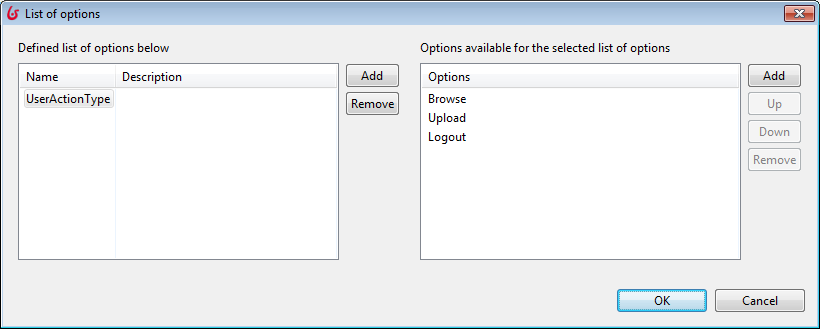
\includegraphics{img/bpmn/bonita_useractiontype.png}
  \caption{The \texttt{UserActionType}}
  \end{figure}
\item
  To create the login screen, click on the \texttt{User workflow}
  \emph{process}. On the \textbf{Application tab}'s \textbf{Entry
  Pageflow} page add a new form named \texttt{Login}.
\item
  In the \textbf{Add widgets based on\ldots{}} groupbox only select the
  \texttt{username} and \texttt{password} widgets.
\item
  Set the password field's \textbf{Field type} to \textbf{Password}.

  \begin{figure}[htbp]
  \centering
  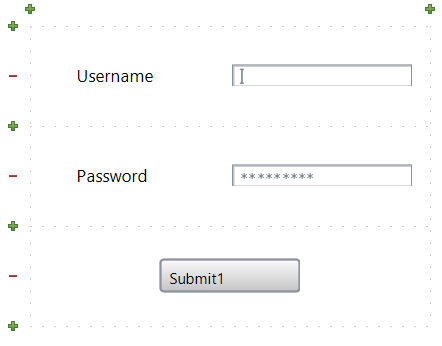
\includegraphics{img/bpmn/bonita_login_screen.png}
  \caption{The login screen}
  \end{figure}
\item
  Connect the \emph{start event} to the \texttt{Authenticate} task. This
  is a service task which simulates the authentication of the user. Add
  a new \textbf{Groovy} connector named
  \texttt{Simulation of Authentication}.

\begin{Shaded}
\begin{Highlighting}[]
\KeywordTok{if} \NormalTok{(username == password) \{}
  \KeywordTok{return} \NormalTok{username.}\FunctionTok{hashCode}\NormalTok{(); }
\NormalTok{\} }\KeywordTok{else} \NormalTok{\{ }
  \KeywordTok{return} \KeywordTok{null}\NormalTok{;}
\NormalTok{\}}
\end{Highlighting}
\end{Shaded}

  The \texttt{result} from connector's output goes to the
  \texttt{user\_ID} variable. Click \textbf{Finish}.
\item
  Depending on the authentication's result, the user can proceed or fail
  the login. Create transitions from the \texttt{Authenticate} task to
  the \texttt{User action} task named \texttt{success} and the
  \texttt{Login failed} task name \texttt{fail}.
\item
  On the \texttt{success} transition choose \textbf{Edit
  expression\ldots{}} in the \textbf{Condition} combobox and type
  \texttt{user\_ID != null}. If this condition is not satisfied, the
  login fails. To implement this, tick the \textbf{Default flow}
  checkbox for the \texttt{fail} transition.
\item
  Add a form to the \texttt{User action} task. Only select the
  \texttt{action} widget, which will be mapped to radio buttons.
\item
  Now we have to create the conditions to the transitions from the XOR
  gateway. To do this, click on the transition and from the
  \textbf{Condition} combobox choose the \textbf{Edit
  expression\ldots{}}.

  \begin{itemize}
  \itemsep1pt\parskip0pt\parsep0pt
  \item
    For the transition to the \texttt{Browse applications} task, set the
    expression to \texttt{action == UserActionType.Browse}. Pay
    attention to import the enumeration -- the Groovy editor is
    basically and Eclipse editor, so you use the content assist
    (\texttt{Ctrl}+\texttt{Space}) to do so.
  \item
    For the transition to the \texttt{Upload application} task, set the
    expression to \texttt{action == UserActionType.Upload}.
  \item
    For the transition to the \texttt{Logout} task, tick the
    \textbf{Default flow} checkbox.
  \end{itemize}
\item
  The user can browse and upload applications multiple times. To
  implement this in the process, we have to create a loop. In order to
  do so, create an \emph{abstract task} named
  \texttt{End of repeatable user action} and create the necessary
  transitions (see the figure).
\item
  For the \texttt{Browse applications} task set the \textbf{Subprocess
  Name} to \texttt{Browse\_Application}.
\item
  Create a form for the \texttt{Logout} task. Add a message saying
  \texttt{The following user has logged out: \$\{username\}}.
\item
  Create a form for the \texttt{Login failed} task. Add a message saying
  \texttt{Login failed}.

  \begin{figure}[htbp]
  \centering
  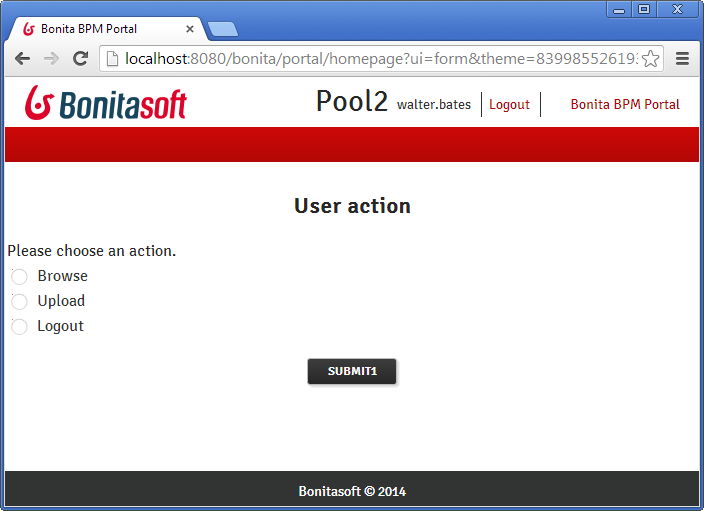
\includegraphics{img/bpmn/bonita_radio_buttons_web.png}
  \caption{The \texttt{user action} form}
  \end{figure}
\item
  From the \texttt{Login failed} and the \texttt{Logout} tasks draw a
  transition to the \emph{end event}.

  \begin{figure}[htbp]
  \centering
  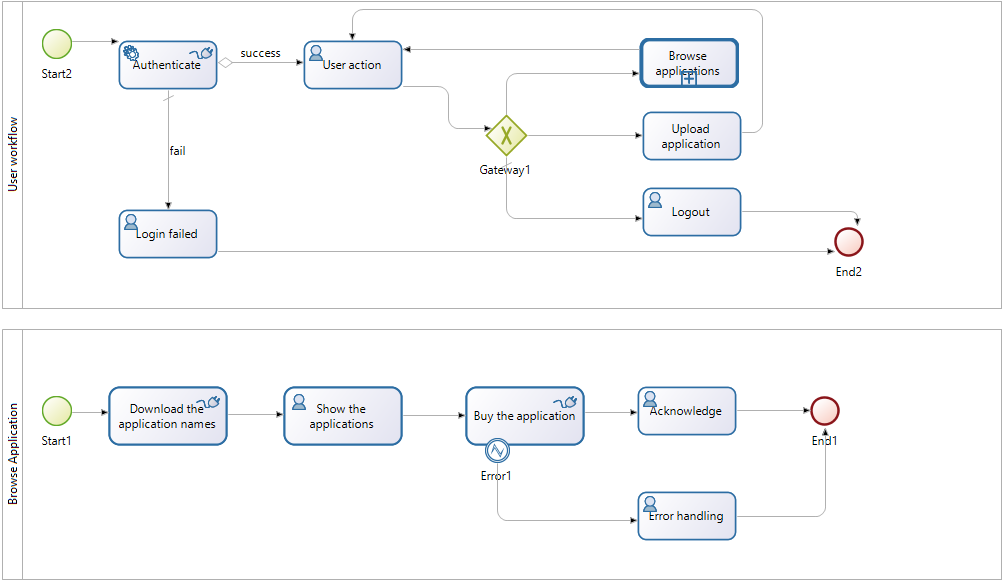
\includegraphics{img/bpmn/bonita_final_workflow.png}
  \caption{The final process}
  \end{figure}
\end{enumerate}

\section{Tips}

\begin{itemize}
\itemsep1pt\parskip0pt\parsep0pt
\item
  If you close some windows by mistakes, you can make them reappear by
  choosing \textbf{View \textbar{} Reset view}.
\item
  If you name a transition and then delete the name, Bonita will mark it
  as faulty with the following message: \textbf{Empty name detected for
  a SequenceFlow}. The solution is to name the transition.
\item
  Sometimes, the error markings don't disappear until you manually
  validate the workflow by clicking \textbf{Process \textbar{}
  Validate}.
\end{itemize}

\chapter{Web services}

\section{Introduction}

In this laboratory, we will create web applications. First, we will
define the data types. We will create a JAX-WS and a JAX-RS web
application and deploy them on a Tomcat server.

\section{Remarks}

For this laboratory, we relied heavily on the Vogella site's
(\url{http://www.vogella.com/}) tutorials. If you're further interested
in the topics, we recommend to study them -- they are thorough and
well-written.

\begin{itemize}
\itemsep1pt\parskip0pt\parsep0pt
\item
  Servlet and JSP development with Eclipse WTP,
  \url{http://www.vogella.com/articles/EclipseWTP/article.html}
\item
  REST with Java (JAX-RS) using Jersey,
  \url{http://www.vogella.com/articles/REST/article.html}
\item
  Apache Tomcat,
  \url{http://www.vogella.com/articles/ApacheTomcat/article.html}
\item
  JAXB, \url{http://www.vogella.com/articles/JAXB/article.html}
\end{itemize}

\section{Apache Tomcat}

From Wikipedia (\url{http://en.wikipedia.org/wiki/Apache_Tomcat}):
,,Apache Tomcat is an open source web server and servlet container
developed by the Apache Software Foundation. Tomcat implements the Java
Servlet and the JavaServer Pages (JSP) specifications from Sun
Microsystems, and provides a ,pure Java' HTTP web server environment for
Java code to run.''

\begin{figure}[htbp]
\centering

\includegraphics{img/web_services/logo.jpg}
\caption{The logo of Tomcat}
\end{figure}

\section{WSDL}

WSDL (Web Services Description Language)

\begin{itemize}
\itemsep1pt\parskip0pt\parsep0pt
\item
  A developer using a bottom up method writes implementing classes
  first, and then uses a WSDL generating tool to expose methods from
  these classes as a Web service. This is simpler to develop but may be
  harder to maintain if the original classes are subject to frequent
  change.
\item
  A developer using a top down method writes the WSDL document first and
  then uses a code generating tool to produce the class skeleton, to be
  completed as necessary. This way is generally considered more
  difficult but can produce cleaner designs and is generally more
  resistant to change. As long as the message formats between sender and
  receiver do not change, changes in the sender and receiver themselves
  do not affect the web-service. The technique is also referred to as
  ``contract first''.
\end{itemize}

\section{JAX-RS}

From Wikipedia
(\url{http://en.wikipedia.org/wiki/Java_API_for_RESTful_Web_Services}):
,,JAX-RS: Java API for RESTful Web Services is a Java programming
language API that provides support in creating web services according to
the Representational State Transfer (REST) architectural style.''

\subsection{Jersey}

To use JAX-RS, we need to use Jersey (\url{http://jersey.java.net/}).
,,Jersey is Sun's production quality reference implementation for JSR
311: JAX-RS: The Java API for RESTful Web Services. Jersey implements
support for the annotations defined in JSR-311, making it easy for
developers to build RESTful web services with Java and the Java JVM.''

\section{JAXB}

From Wikipedia
(\url{http://en.wikipedia.org/wiki/Java_Architecture_for_XML_Binding}):
,,Java Architecture for XML Binding (JAXB) allows Java developers to map
Java classes to XML representations. JAXB provides two main features:
the ability to marshal Java objects into XML and the inverse, i.e.~to
unmarshal XML back into Java objects.''

\section{Maven}

From Wikipedia (\url{http://en.wikipedia.org/wiki/Apache_Maven}):
,,Maven is a build automation tool used primarily for Java projects.
Maven uses an XML file to describe the software project being built, its
dependencies on other external modules and components, the build order,
directories, and required plug-ins. Maven dynamically downloads Java
libraries and Maven plug-ins from one or more repositories such as the
Maven 2 Central Repository, and stores them in a local cache. This local
cache of downloaded artifacts can also be updated with artifacts created
by local projects. Public repositories can also be updated.''

\chapter{Web services laboratory -- step-by-step instructions}

\section{Prerequisites}

To create a basic web service in Eclipse, you need to install some
plug-ins.

\subsection{Eclipse WTP}

Eclipse provides a bunch of plug-ins called \emph{Web Tools Platform}
(WTP) to aid the development of web services.

\begin{enumerate}
\def\labelenumi{\arabic{enumi}.}
\item
  Click \textbf{Help \textbar{} Install New Software}. From the
  \textbf{Work with} combobox pick \textbf{Juno}. From the category
  ``Web, XML, Java EE Development and OSGi Enterprise Development''
  install the following packages:

  \begin{itemize}
  \itemsep1pt\parskip0pt\parsep0pt
  \item
    Eclipse XML Editors and Tools

    \begin{itemize}
    \itemsep1pt\parskip0pt\parsep0pt
    \item
      XML editor, highligher, etc.
    \end{itemize}
  \item
    JST Server Adapters Extensions

    \begin{itemize}
    \itemsep1pt\parskip0pt\parsep0pt
    \item
      This is needed to connect to Apache Tomcat
    \end{itemize}
  \item
    Eclipse Java EE Developer Tools
  \item
    Eclipse Java Web Developer Tools

    \begin{itemize}
    \itemsep1pt\parskip0pt\parsep0pt
    \item
      These two are needed to create Dynamic Web Projects.
    \end{itemize}
  \end{itemize}
\item
  Restart Eclipse.
\item
  Click \textbf{Window \textbar{} Preferences}. Pick \textbf{Server
  \textbar{} Runtime Environtment} and click the \textbf{Add\ldots{}}
  button.
\item
  Choose \textbf{Apache \textbar{} Apache Tomcat v7.0}.

  \begin{figure}[htbp]
  \centering
  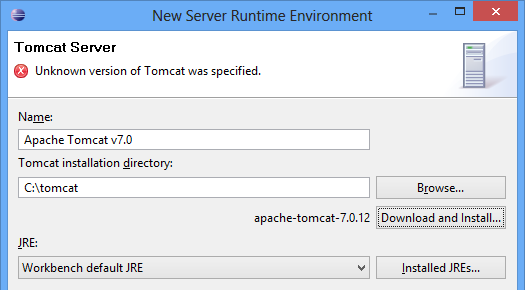
\includegraphics{img/web_services/install_1.png}
  \caption{An error message is displayed while installing Tomcat}
  \end{figure}
\item
  Click \textbf{Next}. Change the name to \texttt{MDSD Tomcat}. Click
  \textbf{Download and install\ldots{}} and choose the installation
  location. Wait for the installation to complete: the \emph{Unknown
  version of Tomcat was specified.} error message will disappear.

  \begin{figure}[htbp]
  \centering
  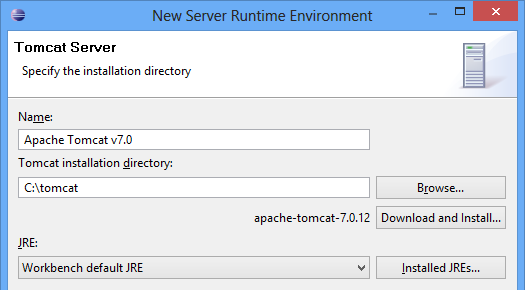
\includegraphics{img/web_services/install_2.png}
  \caption{After the installation is completed, the error message
  disappears}
  \end{figure}
\item
  Click \textbf{Finish}.
\item
  Click \textbf{OK}.
\end{enumerate}

\subsection{Maven}

We will use Maven to resolve the Java dependencies of our software. To
install Maven, install the \textbf{m2e - Maven integration for Eclipse}
package from the \textbf{Juno} update site.

\section{Datatypes}

\begin{enumerate}
\def\labelenumi{\arabic{enumi}.}
\item
  Create a Java project named \texttt{hu.bme.mit.inf.appstore.data}.
\item
  Create a package named \texttt{hu.bme.mit.inf.appstore.data.model} and
  add a class named \texttt{Application}.

\begin{Shaded}
\begin{Highlighting}[]
\KeywordTok{public} \KeywordTok{class} \NormalTok{Application \{}
  \KeywordTok{private} \DataTypeTok{int} \NormalTok{id;}
  \KeywordTok{private} \NormalTok{String name;}
\NormalTok{\}}
\end{Highlighting}
\end{Shaded}
\item
  Add getter/setter methods to the class and generate a constructor that
  uses the \texttt{name} attribute as a parameter.
\item
  We will create a data provider for the model. Create a package named
  \texttt{hu.bme.mit.inf.appstore.data.provider} and add a class named
  \texttt{ApplicationProvider}.

\begin{Shaded}
\begin{Highlighting}[]
\KeywordTok{package hu.bme.mit.inf.appstore.data.provider;}

\KeywordTok{import hu.bme.mit.inf.appstore.data.model.Application;}

\KeywordTok{import java.util.ArrayList;}
\KeywordTok{import java.util.HashMap;}
\KeywordTok{import java.util.List;}
\KeywordTok{import java.util.Map;}

\KeywordTok{public} \KeywordTok{enum} \NormalTok{ApplicationProvider \{}
  \NormalTok{instance;}

  \KeywordTok{private} \NormalTok{Map<Integer, Application> map = }\KeywordTok{new} \NormalTok{HashMap<>();}
  \KeywordTok{private} \DataTypeTok{int} \NormalTok{lastId = }\DecValTok{0}\NormalTok{;}

  \KeywordTok{public} \NormalTok{Application }\FunctionTok{getApplication}\NormalTok{(}\DataTypeTok{int} \NormalTok{id) \{}
    \KeywordTok{return} \NormalTok{map.}\FunctionTok{get}\NormalTok{(id);     }
  \NormalTok{\}}

  \KeywordTok{public} \NormalTok{List<Application> }\FunctionTok{getApplications}\NormalTok{() \{}
    \KeywordTok{return} \KeywordTok{new} \NormalTok{ArrayList<>(map.}\FunctionTok{values}\NormalTok{());}
  \NormalTok{\}}

  \KeywordTok{public} \DataTypeTok{void} \FunctionTok{insertApplication}\NormalTok{(Application application) \{}
      \NormalTok{lastId++;}
      \NormalTok{application.}\FunctionTok{setId}\NormalTok{(lastId);}
      \NormalTok{map.}\FunctionTok{put}\NormalTok{(lastId, application);}
  \NormalTok{\}}


  \FunctionTok{ApplicationProvider}\NormalTok{() \{}
    \FunctionTok{insertApplication}\NormalTok{(}\KeywordTok{new} \FunctionTok{Application}\NormalTok{(}\StringTok{"Flashlight"}\NormalTok{));}
    \FunctionTok{insertApplication}\NormalTok{(}\KeywordTok{new} \FunctionTok{Application}\NormalTok{(}\StringTok{"Weather"}\NormalTok{));}
  \NormalTok{\}}
\NormalTok{\}}
\end{Highlighting}
\end{Shaded}

  We implemented the Singleton pattern with an enumeration. See
  \url{http://www.vogella.com/articles/DesignPatternSingleton/article.html}
  or Joshua Bloch's book \emph{Effective Java} for more details.
\end{enumerate}

If you want to add use the \texttt{Application} class from an other
project, go to the project \textbf{Properties}, \textbf{Java Build
Path}. On the \textbf{Projects} tab click \textbf{Add\ldots{}} and tick
\textbf{hu.bme.mit.inf.appstore.data}.

\section{JAX-WS}

Further reading:
\url{http://wiki.eclipse.org/Creating_a_Bottom-Up_Java_Web_Service}

,,The Java API for XML Web Services (JAX-WS) is a Java programming
language API for creating web services.''

\begin{enumerate}
\def\labelenumi{\arabic{enumi}.}
\item
  Create a new \textbf{Dynamic Web Project} called
  \texttt{hu.bme.mit.inf.appstore.server.ws}. When using the \textbf{New
  Dynamic Web Project} wizard, tick the \textbf{Generate web.xml
  deployment descriptor} checkbox. The \texttt{web.xml} file will be
  generated in the \texttt{WebContent/WEB-INF} directory.

  Remarks:

  \begin{itemize}
  \itemsep1pt\parskip0pt\parsep0pt
  \item
    If you forgot to generate the \texttt{web.xml} file, go to the
    \textbf{Project Explorer}, right click the project name and choose
    \textbf{Java EE Tools \textbar{} Generate deployment descriptor
    stub}.
  \item
    Unlike other natures (like the Plug-in Project and the Maven
    Project), the Dynamic Web Project nature cannot be added to the
    project from the -- you have to start from a Dynamic Web Project and
    add other natures later.
  \end{itemize}
\item
  Eclipse prompts if it should switch to the \textbf{Java EE
  perspective}: choose \textbf{No}.
\item
  Add a dependency to the \texttt{hu.bme.mit.inf.appstore.data} project
  (see the \emph{Datatypes} section for more information).
\item
  Create a new package called \texttt{hu.bme.mit.inf.appstore.server.ws}
  and a new class called \texttt{ApplicationManager}:

\begin{Shaded}
\begin{Highlighting}[]
\KeywordTok{package hu.bme.mit.inf.appstore.server.ws;}

\KeywordTok{import java.util.List;}

\KeywordTok{import hu.bme.mit.inf.appstore.data.model.Application;}
\KeywordTok{import hu.bme.mit.inf.appstore.data.provider.ApplicationProvider;}

\KeywordTok{public} \KeywordTok{class} \NormalTok{ApplicationManager \{}

  \KeywordTok{public} \NormalTok{Application }\FunctionTok{getApplication}\NormalTok{(}\DataTypeTok{int} \NormalTok{id) \{}
    \KeywordTok{return} \NormalTok{ApplicationProvider.}\FunctionTok{instance}\NormalTok{.}\FunctionTok{getApplication}\NormalTok{(id);}
  \NormalTok{\}}

  \KeywordTok{public} \NormalTok{Application[] }\FunctionTok{getApplications}\NormalTok{() \{}
    \NormalTok{List<Application> list = ApplicationProvider.}\FunctionTok{instance}\NormalTok{.}\FunctionTok{getApplications}\NormalTok{();}
    \NormalTok{Application[] array = list.}\FunctionTok{toArray}\NormalTok{(}\KeywordTok{new} \NormalTok{Application[list.}\FunctionTok{size}\NormalTok{()]); }
    \KeywordTok{return} \NormalTok{array;}
  \NormalTok{\}}

  \KeywordTok{public} \DataTypeTok{void} \FunctionTok{insertApplication}\NormalTok{(Application application) \{}
    \NormalTok{ApplicationProvider.}\FunctionTok{instance}\NormalTok{.}\FunctionTok{insertApplication}\NormalTok{(application);}
  \NormalTok{\}}
\NormalTok{\}}
\end{Highlighting}
\end{Shaded}
\item
  Right click the project and choose \textbf{Web Services \textbar{}
  Create Web Service}. This will generate the description files and the
  client application, then deploy the application on the server.

  \begin{itemize}
  \itemsep1pt\parskip0pt\parsep0pt
  \item
    \textbf{Web service type}: \textbf{Bottom up Java Bean Service}
  \item
    \textbf{Service implementation}:
    \texttt{hu.bme.mit.inf.appstore.server.ws.ApplicationManager}
  \item
    Server level: \textbf{Start service}
  \item
    \textbf{Client type}: \textbf{Java proxy}
  \item
    Client level: \textbf{Test client}
  \end{itemize}

  Tick the \textbf{Monitor the Web service} checkbox.

  Go through the pages with the \textbf{Next} button and click
  \textbf{Finish}.

  \begin{figure}[htbp]
  \centering
  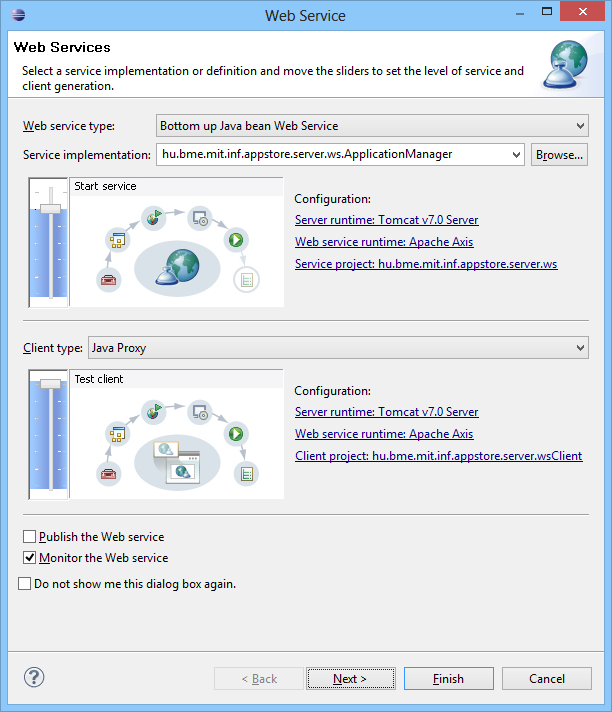
\includegraphics{img/web_services/web_service_wizard.png}
  \caption{The \textbf{Web Service} wizard}
  \end{figure}
\item
  While deploying, you will get a warning that the \texttt{Application}
  class does not have a default no-arg contructor.

  Create a default constructor (a constructor with no arguments, hence
  often referred as \emph{no-arg constructor}) to the
  \texttt{Application} class.
\item
  While deploying, Tomcat will throw the following exception:

  \texttt{org.apache.axis.deployment.wsdd.WSDDNonFatalException: java.lang.ClassNotFoundException}

  The reason is that the dependencies (i.e.~the
  \texttt{hu.bme.mit.inf.appstore.data} project) are only available at
  compile time, but not avaiable at runtime. To correct this, go to the
  project's \textbf{Properties} window, choose \textbf{Deployment
  Assembly} page. Click \textbf{Add\ldots{}}, \textbf{Project},
  \texttt{hu.bme.mit.inf.appstore.data}.
\item
  Use \textbf{Create Web Service} again and deploy the server.
\item
  Insert a new application with the \texttt{insertApplication()} method.
  The following XML envelope is generated:

\begin{Shaded}
\begin{Highlighting}[]
\KeywordTok{<?xml} \NormalTok{version="1.0" encoding="UTF-8" standalone="no"}\KeywordTok{?>}
\KeywordTok{<soapenv:Envelope} 
\OtherTok{  xmlns:soapenv=}\StringTok{"http://schemas.xmlsoap.org/soap/envelope/"} 
\OtherTok{  xmlns:xsd=}\StringTok{"http://www.w3.org/2001/XMLSchema"} 
\OtherTok{  xmlns:xsi=}\StringTok{"http://www.w3.org/2001/XMLSchema-instance"}\KeywordTok{>}
  \KeywordTok{<soapenv:Body>}
    \KeywordTok{<insertApplication}\OtherTok{ xmlns=}\StringTok{"http://ws.server.appstore.inf.mit.bme.hu"}\KeywordTok{>}
      \KeywordTok{<application>}
        \KeywordTok{<ns1:id}\OtherTok{ xmlns:ns1=}\StringTok{"http://model.data.appstore.inf.mit.bme.hu"}\KeywordTok{>}\NormalTok{3}\KeywordTok{</ns1:id>}
        \KeywordTok{<ns2:name}\OtherTok{ xmlns:ns2=}\StringTok{"http://model.data.appstore.inf.mit.bme.hu"}\KeywordTok{>}\NormalTok{News}\KeywordTok{</ns2:name>}
      \KeywordTok{</application>}
    \KeywordTok{</insertApplication>}
  \KeywordTok{</soapenv:Body>}
\KeywordTok{</soapenv:Envelope>}
\end{Highlighting}
\end{Shaded}
\item
  List the application with the \texttt{getApplications()} method.
\item
  You can observe the traffic in the \textbf{TCP/IP Monitor}. To make
  the XML messages more readable, change \textbf{Byte} to \textbf{Web
  Browser} for both the \textbf{Request} and the \textbf{Response}
  messages.

  \begin{figure}[htbp]
  \centering
  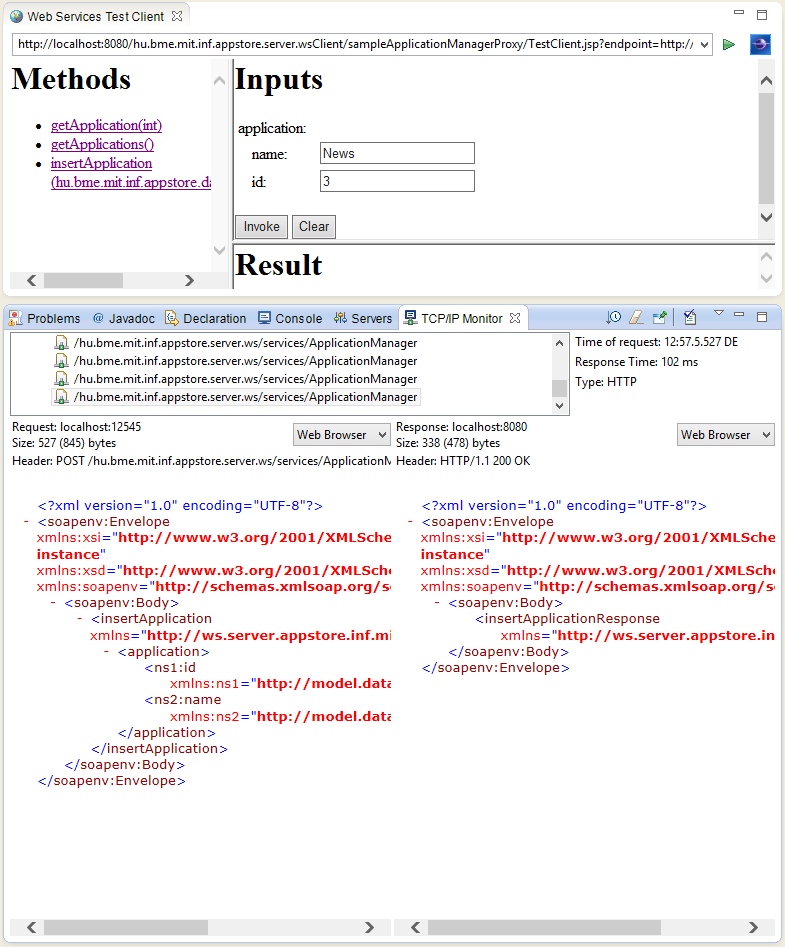
\includegraphics{img/web_services/tcp_ip_monitor_insert.png}
  \caption{Inserting a new application to the application store}
  \end{figure}

  \begin{figure}[htbp]
  \centering
  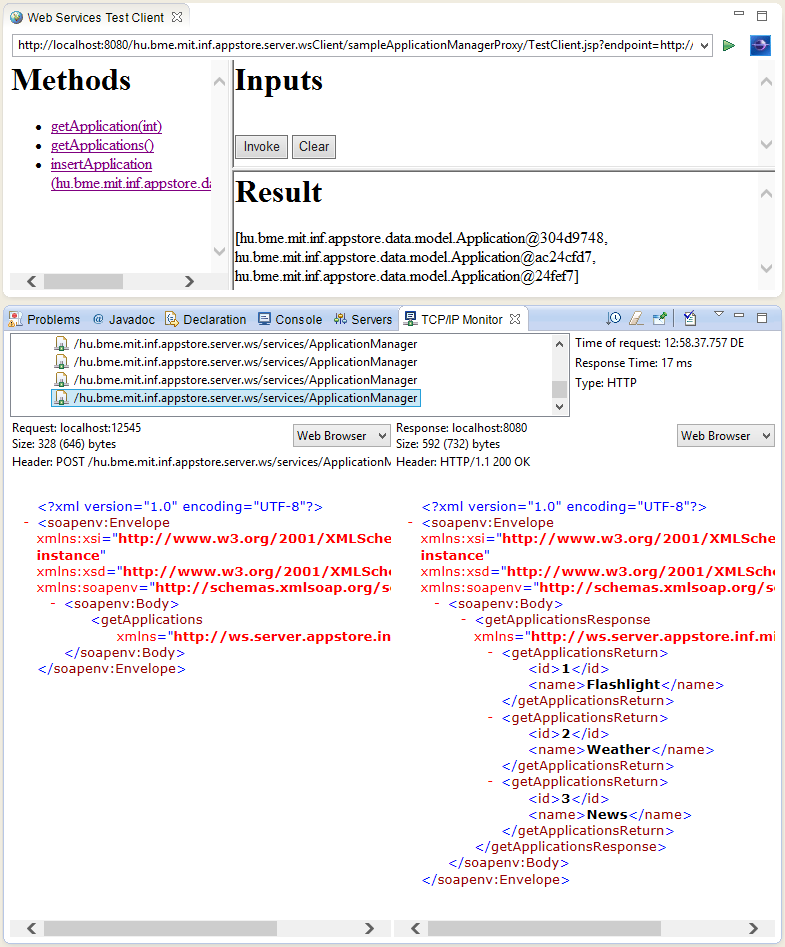
\includegraphics{img/web_services/tcp_ip_monitor_list.png}
  \caption{Listing the applications from the application store}
  \end{figure}
\end{enumerate}

\section{JAX-RS}

\subsection{Creating the project}

\begin{enumerate}
\def\labelenumi{\arabic{enumi}.}
\item
  Create a new \textbf{Dynamic Web Project} called
  \texttt{hu.bme.mit.inf.appstore.server.rest}. When using the
  \textbf{New Dynamic Web Project} wizard, tick the \textbf{Generate
  web.xml deployment descriptor} checkbox. The \texttt{web.xml} file
  will be generated in the \texttt{WebContent/WEB-INF} directory.

  Set the \textbf{Context root} to \texttt{appstore}.
\item
  Eclipse prompts if it should switch to the \textbf{Java EE
  perspective}: choose \textbf{No}.
\end{enumerate}

\subsection{Dependencies}

To use create REST services, we have to use Jersey. Jersey is the
reference implementation for the JAX-RS specification.

\begin{enumerate}
\def\labelenumi{\arabic{enumi}.}
\item
  We use Maven to resolve the dependencies. In order to use Maven, we
  need to add the Maven nature to the project. Right click the project
  and pick \textbf{Configure \textbar{} Convert to Maven Project}. The
  default artifact settings are fine, click \textbf{Finish}.
\item
  Click the \texttt{pom.xml} file and choose the last tab, named
  \textbf{pom.xml}.

  To specify the dependencies, add the following code under the
  \texttt{\textless{}project\textgreater{}} element:

\begin{Shaded}
\begin{Highlighting}[]
\KeywordTok{<dependencies>}
  \KeywordTok{<dependency>}
    \KeywordTok{<groupId>}\NormalTok{com.sun.jersey}\KeywordTok{</groupId>}
    \KeywordTok{<artifactId>}\NormalTok{jersey-server}\KeywordTok{</artifactId>}
    \KeywordTok{<version>}\NormalTok{1.17}\KeywordTok{</version>}
  \KeywordTok{</dependency>}
  \KeywordTok{<dependency>}
    \KeywordTok{<groupId>}\NormalTok{com.sun.jersey}\KeywordTok{</groupId>}
    \KeywordTok{<artifactId>}\NormalTok{jersey-bundle}\KeywordTok{</artifactId>}
    \KeywordTok{<version>}\NormalTok{1.17}\KeywordTok{</version>}
  \KeywordTok{</dependency>}
\KeywordTok{</dependencies>}
\end{Highlighting}
\end{Shaded}
\end{enumerate}

\subsection{Java code}

\begin{enumerate}
\def\labelenumi{\arabic{enumi}.}
\item
  Create a package named \texttt{hu.bme.mit.inf.appstore.server.rest}
  and a class named \texttt{Hello}.

\begin{Shaded}
\begin{Highlighting}[]
\KeywordTok{package hu.bme.mit.inf.appstore.server.rest;}

\KeywordTok{import javax.ws.rs.GET;}
\KeywordTok{import javax.ws.rs.Path;}

\FunctionTok{@Path}\NormalTok{(}\StringTok{"hello"}\NormalTok{)}
\KeywordTok{public} \KeywordTok{class} \NormalTok{Hello \{}

  \FunctionTok{@GET}
  \KeywordTok{public} \NormalTok{String }\FunctionTok{sayHello}\NormalTok{() \{}
    \KeywordTok{return} \StringTok{"Hello"}\NormalTok{;}
  \NormalTok{\}}

\NormalTok{\}}
\end{Highlighting}
\end{Shaded}
\end{enumerate}

\subsection{Deployment}

\begin{enumerate}
\def\labelenumi{\arabic{enumi}.}
\item
  Edit the \texttt{web.xml} file in the \texttt{WebContent/WEB-INF}
  directory. Delete the content of the
  \texttt{\textless{}web-app\textgreater{}} element and paste the
  following:

\begin{Shaded}
\begin{Highlighting}[]
\KeywordTok{<display-name></display-name>}
\KeywordTok{<servlet>}
  \KeywordTok{<servlet-name></servlet-name>}
  \KeywordTok{<servlet-class>}\NormalTok{com.sun.jersey.spi.container.servlet.ServletContainer}\KeywordTok{</servlet-class>}
  \KeywordTok{<init-param>}
    \KeywordTok{<param-name>}\NormalTok{com.sun.jersey.config.property.packages}\KeywordTok{</param-name>}
    \KeywordTok{<param-value></param-value>}
  \KeywordTok{</init-param>}
  \KeywordTok{<load-on-startup>}\NormalTok{1}\KeywordTok{</load-on-startup>}
\KeywordTok{</servlet>}
\KeywordTok{<servlet-mapping>}
  \KeywordTok{<servlet-name></servlet-name>}
  \KeywordTok{<url-pattern></url-pattern>}
\KeywordTok{</servlet-mapping>}
\end{Highlighting}
\end{Shaded}

  Fill the elements according to the following table:

  \begin{longtable}[c]{@{}ll@{}}
  \hline\noalign{\medskip}
  \texttt{display-name} & \texttt{Application Store}
  \\\noalign{\medskip}
  \texttt{servlet-name} (2×) & \texttt{Application Store REST Service}
  \\\noalign{\medskip}
  \texttt{param-value} & \texttt{hu.bme.mit.inf.appstore.server.rest}
  \\\noalign{\medskip}
  \texttt{url-pattern} & \texttt{/rest/*}
  \\\noalign{\medskip}
  \hline
  \end{longtable}
\item
  Start the server. Tomcat will throw the following exception:

\begin{verbatim}
SEVERE: Servlet /hu.bme.mit.inf.appstore.server.rest threw load() exception
java.lang.ClassNotFoundException: com.sun.jersey.spi.container.servlet.ServletContainer
\end{verbatim}

  The reason for this is that Eclipse not deploy dependencies (JAR
  files) resolved by Maven to the web application. To correct this, go
  to the project's \textbf{Properties} window, choose \textbf{Deployment
  Assembly} page. Click \textbf{Add\ldots{}}, \textbf{Java Build Path
  Entries}, \textbf{Maven Dependencies}.

  \begin{figure}[htbp]
  \centering
  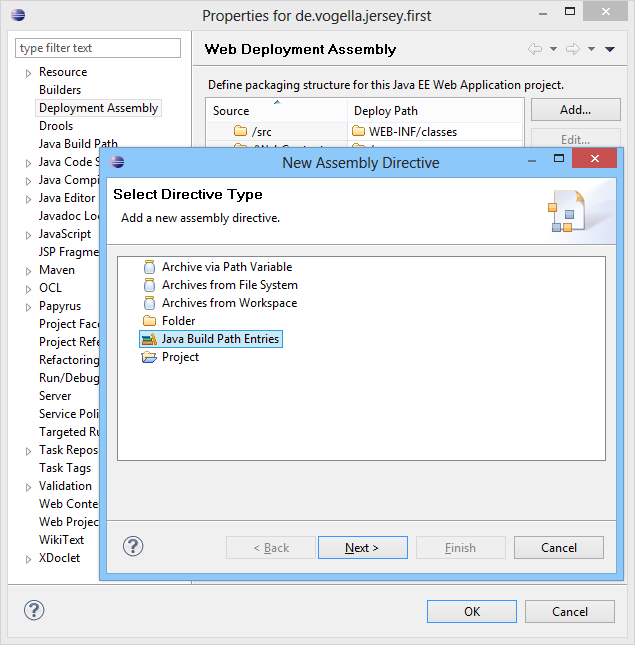
\includegraphics{img/web_services/deployment_assembly.png}
  \caption{\textbf{Deployment Assembly}}
  \end{figure}

  If you don't use Maven, you have to put the JAR files to the
  \texttt{WebContent/WEB-INF/lib} directory and add them to the
  project's build path.
\item
  Start the server. It will start but the browser in Eclipse will show a
  page with a 404 error. Let's examine ho the URL of the REST service is
  built:

\begin{verbatim}
http://domain:port/context-root/url-pattern/path-from-REST-class
\end{verbatim}

  The \texttt{context-root} is defined in the
  \texttt{org.eclipse.wst.common.component} file, the
  \texttt{url-pattern} is defined in the \texttt{web.xml} file and the
  \texttt{path-from-REST-class} is defined in the Java source file.

  Remark: the Vogella JAX-RS tutorial is wrong on this point. The
  \texttt{display-name} in the \texttt{web.xml} file only sets the name
  of the application (which is shown in the Web Application Manager). It
  has nothing to do with the URL of the application.
\item
  If you want to change the \texttt{context-root}, go to the project
  \textbf{Properties}. On the \textbf{Web Project Settings} set the
  \textbf{Context root}.

  To check if it worked, go to the \texttt{.settings} directory and edit
  the \texttt{org.eclipse.wst.common.component} file.

\begin{Shaded}
\begin{Highlighting}[]
\KeywordTok{<?xml} \NormalTok{version="1.0" encoding="UTF-8"}\KeywordTok{?>}
\KeywordTok{<project-modules}\OtherTok{ id=}\StringTok{"moduleCoreId"}\OtherTok{ project-version=}\StringTok{"1.5.0"}\KeywordTok{>}
  \KeywordTok{<wb-module}\OtherTok{ deploy-name=}\StringTok{"[deployment-name]"}\KeywordTok{>}
    \KeywordTok{<wb-resource}\OtherTok{ deploy-path=}\StringTok{"/"}\OtherTok{ source-path=}\StringTok{"/WebContent"}\OtherTok{ tag=}\StringTok{"defaultRootSource"} \KeywordTok{/>}
    \KeywordTok{<wb-resource}\OtherTok{ deploy-path=}\StringTok{"/WEB-INF/classes"}\OtherTok{ source-path=}\StringTok{"/src"} \KeywordTok{/>}
    \KeywordTok{<property}\OtherTok{ name=}\StringTok{"context-root"}\OtherTok{ value=}\StringTok{"[context-root]"} \KeywordTok{/>}
    \KeywordTok{<property}\OtherTok{ name=}\StringTok{"java-output-path"}\OtherTok{ value=}\StringTok{"/[java-output-path]/build/classes"} \KeywordTok{/>}
  \KeywordTok{</wb-module>}
\KeywordTok{</project-modules>}
\end{Highlighting}
\end{Shaded}

  For now, leave the \texttt{{[}deploy-name{]}} and the
  \texttt{{[}java-output-path{]}} fields as they are.
\item
  If the server is running, stop it. Remove the application (right
  click, \textbf{Remove}) and restart the application. The URL's
  \texttt{context-root} will be set to the new one.

  Remark: if this does not work as expected (e.g.~the path in the Tomcat
  Web Application Manager is still the same), stop the server, run a
  clean operation (right click, \textbf{Clean\ldots{}}) and start again.
\end{enumerate}

\section{JAXB}

We will continue to work with the
\texttt{hu.bme.mit.inf.appstore.server.rest} project and add JAXB
support to it. This way, we send and receive Java objects serialized to
XML.

\begin{enumerate}
\def\labelenumi{\arabic{enumi}.}
\item
  Add a dependency to the \texttt{hu.bme.mit.inf.appstore.data} project
  (see the \emph{Datatypes} section for more information).
\item
  Add the \texttt{@XmlRootElement} annotation to the
  \texttt{Application} class.

\begin{Shaded}
\begin{Highlighting}[]
\FunctionTok{@XmlRootElement}
\KeywordTok{public} \KeywordTok{class} \NormalTok{Application \{}
  \CommentTok{// ...}
\NormalTok{\}}
\end{Highlighting}
\end{Shaded}
\item
  If you didn't do so already, add a default constructor to the
  \texttt{Application} class.
\item
  Create a new class named \texttt{ApplicationManager}:

\begin{Shaded}
\begin{Highlighting}[]
\KeywordTok{package hu.bme.mit.inf.appstore.server.rest;}

\KeywordTok{import hu.bme.mit.inf.appstore.data.model.Application;}
\KeywordTok{import hu.bme.mit.inf.appstore.data.provider.ApplicationProvider;}

\KeywordTok{import java.util.List;}

\KeywordTok{import javax.ws.rs.Consumes;}
\KeywordTok{import javax.ws.rs.GET;}
\KeywordTok{import javax.ws.rs.POST;}
\KeywordTok{import javax.ws.rs.Path;}
\KeywordTok{import javax.ws.rs.PathParam;}
\KeywordTok{import javax.ws.rs.Produces;}
\KeywordTok{import javax.ws.rs.core.Context;}
\KeywordTok{import javax.ws.rs.core.MediaType;}
\KeywordTok{import javax.ws.rs.core.Response;}
\KeywordTok{import javax.ws.rs.core.UriInfo;}

\FunctionTok{@Path}\NormalTok{(}\StringTok{"applicationmanager"}\NormalTok{)}
\KeywordTok{public} \KeywordTok{class} \NormalTok{ApplicationManager \{}

  \FunctionTok{@Context}
  \KeywordTok{private} \NormalTok{UriInfo uriInfo;}

  \FunctionTok{@GET}
  \FunctionTok{@Path}\NormalTok{(}\StringTok{"list"}\NormalTok{)}
  \FunctionTok{@Produces}\NormalTok{(\{ MediaType.}\FunctionTok{APPLICATION_XML}\NormalTok{, MediaType.}\FunctionTok{APPLICATION_JSON} \NormalTok{\})}
  \KeywordTok{public} \NormalTok{List<Application> }\FunctionTok{getApplications}\NormalTok{() \{}
    \KeywordTok{return} \NormalTok{ApplicationProvider.}\FunctionTok{instance}\NormalTok{.}\FunctionTok{getApplications}\NormalTok{();}
  \NormalTok{\}}

  \FunctionTok{@GET}
  \FunctionTok{@Path}\NormalTok{(}\StringTok{"get/\{id\}"}\NormalTok{)}
  \FunctionTok{@Produces}\NormalTok{(\{ MediaType.}\FunctionTok{APPLICATION_XML}\NormalTok{, MediaType.}\FunctionTok{APPLICATION_JSON} \NormalTok{\})}
  \KeywordTok{public} \NormalTok{Application }\FunctionTok{getApplication}\NormalTok{(}\FunctionTok{@PathParam}\NormalTok{(}\StringTok{"id"}\NormalTok{) }\DataTypeTok{int} \NormalTok{id) \{}
    \NormalTok{Application application = ApplicationProvider.}\FunctionTok{instance}\NormalTok{.}\FunctionTok{getApplication}\NormalTok{(id);}
    \KeywordTok{return} \NormalTok{application;}
  \NormalTok{\}}

  \FunctionTok{@POST}
  \FunctionTok{@Path}\NormalTok{(}\StringTok{"insert"}\NormalTok{)}
  \FunctionTok{@Consumes}\NormalTok{(MediaType.}\FunctionTok{APPLICATION_XML}\NormalTok{)}
  \KeywordTok{public} \NormalTok{Response }\FunctionTok{insertApplication}\NormalTok{(Application application) \{}
    \NormalTok{ApplicationProvider.}\FunctionTok{instance}\NormalTok{.}\FunctionTok{insertApplication}\NormalTok{(application);}
    \KeywordTok{return} \NormalTok{Response.}\FunctionTok{created}\NormalTok{(uriInfo.}\FunctionTok{getAbsolutePath}\NormalTok{()).}\FunctionTok{build}\NormalTok{();}
  \NormalTok{\}}

\NormalTok{\}}
\end{Highlighting}
\end{Shaded}
\end{enumerate}

\section{Tomcat Web Application Manager}

Tomcat has an administration page called \textbf{Tomcat Web Application
Manager}. However, it will not work if Tomcat is launched with Eclipse's
default settings. To make it work, click the server in the
\textbf{Servers} view.

You have to change the \textbf{Server Location} from \textbf{Use
workspace metadata} to \textbf{Use Tomcat installation}. If you have
already started an application on the server, the radiobuttons will be
disabled. To enable them stop the server (right click, \textbf{Stop})
and do a clean operation (right click, \textbf{Clean\ldots{}}). After
that, the radiobuttons should be enabled again.

\begin{figure}[htbp]
\centering
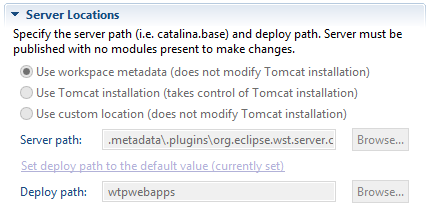
\includegraphics{img/web_services/server_settings_1.png}
\caption{If you have already deployed an application, the \textbf{Server
Location} radiobuttons are disabled}
\end{figure}

\begin{figure}[htbp]
\centering
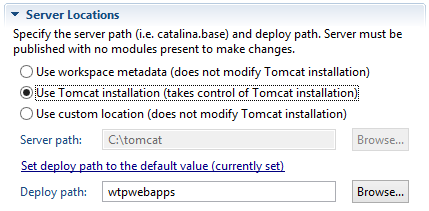
\includegraphics{img/web_services/server_settings_2.png}
\caption{Choose the \textbf{Use Tomcat installation} option}
\end{figure}

Start the server. Now you can access the Tomcat Web Application Manager
on \url{http://localhost:8080/manager/html}. However, you can't log in
yet: you have to define a user. To do so, go to the Tomcat installation
directory and add the following to the \texttt{conf/tomcat-users.xml}
file's \texttt{\textless{}tomcat-users\textgreater{}} element:

\begin{Shaded}
\begin{Highlighting}[]
\KeywordTok{<role}\OtherTok{ rolename=}\StringTok{"manager-gui"}\KeywordTok{/>}
\KeywordTok{<user}\OtherTok{ name=}\StringTok{"admin"}\OtherTok{ password=}\StringTok{"admin"}\OtherTok{ roles=}\StringTok{"admin-gui,manager-gui"}\KeywordTok{/>}
\end{Highlighting}
\end{Shaded}

You should be able to login with the user \texttt{admin} and the
password \texttt{admin}.

\begin{figure}[htbp]
\centering
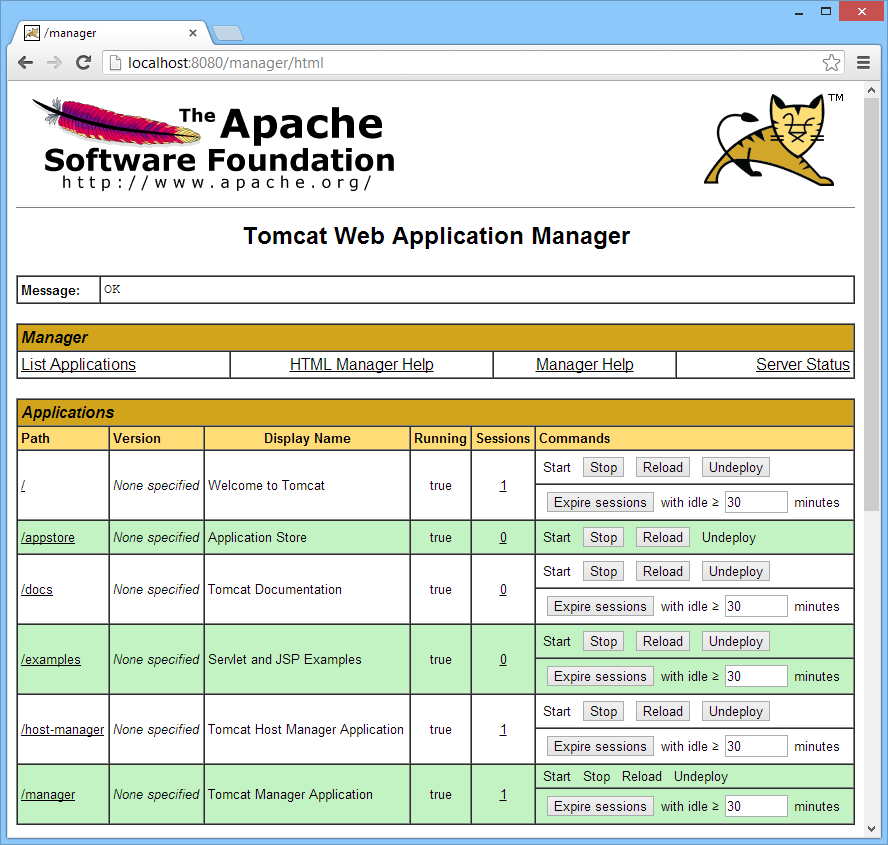
\includegraphics{img/web_services/web_application_manager.png}
\caption{The Tomcat Web Application Manager listing the
\texttt{appstore} application}
\end{figure}

\subsection{Performance monitoring}

If you want to monitor the performance of Tomcat, you can use JConsole
(\url{http://docs.oracle.com/javase/7/docs/technotes/guides/management/jconsole.html}).
JConsole can monitor applications that are compatible with Java
Management Extensions (JMX) specification. You can find JConsole in your
JDK's \texttt{bin} directory.

If you want to measure the performance of a web server, e.g.~Apache
Tomcat, you should use a performance testing tool like Apache JMeter
(\url{http://jmeter.apache.org/}). JMeter is used in the \emph{Design
for Dependability Laboratory Exercises}
(\url{http://www.inf.mit.bme.hu/edu/courses/szbtlab}) course of the
,,Dependable System Design'' programme held in the autumn semester.

Further reading:

\begin{itemize}
\itemsep1pt\parskip0pt\parsep0pt
\item
  \url{http://stackoverflow.com/questions/787070/how-to-properly-manage-tomcat-web-apps-inside-eclipse}
\item
  \url{http://stackoverflow.com/questions/6776421/display-the-tomcat-manager-application}
\item
  \url{http://stackoverflow.com/questions/2280064/tomcat-started-in-eclipse-but-unable-to-connect-to-link-to-http-localhost8085}
\item
  \url{http://tomcat.apache.org/tomcat-7.0-doc/html-manager-howto.html}
\end{itemize}

\section{Testing a REST application}

The simplicity of the REST style enables us to test REST applications
without writing our own test client. Advanced Rest Client
(\url{http://chromerestclient.appspot.com/}) is an extension for Google
Chrome. Advanced Rest Client is capable of sending requests to REST
applications with a specific HTTP method (e.g.~GET, POST, etc.) and a
header. This way, you can emulate the behaviour of a client application.

\begin{itemize}
\item
  \url{http://localhost:8080/appstore/rest/applicationmanager/get/2},
  HTTP method: GET
\item
  \url{http://localhost:8080/appstore/rest/applicationmanager/insert},
  HTTP method: POST.

  Use the following payload:

\begin{Shaded}
\begin{Highlighting}[]
\KeywordTok{<application>}
  \KeywordTok{<name>}\NormalTok{News}\KeywordTok{</name>}
\KeywordTok{</application>}
\end{Highlighting}
\end{Shaded}

  Create a \texttt{Content-Type} field in the header and set it to
  \texttt{application/xml}.
\item
  \url{http://localhost:8080/appstore/rest/applicationmanager/list},
  HTTP method: GET.

  Create an \texttt{Accept} field in the header and set it to
  \texttt{application/json}.
\end{itemize}

\begin{figure}[htbp]
\centering
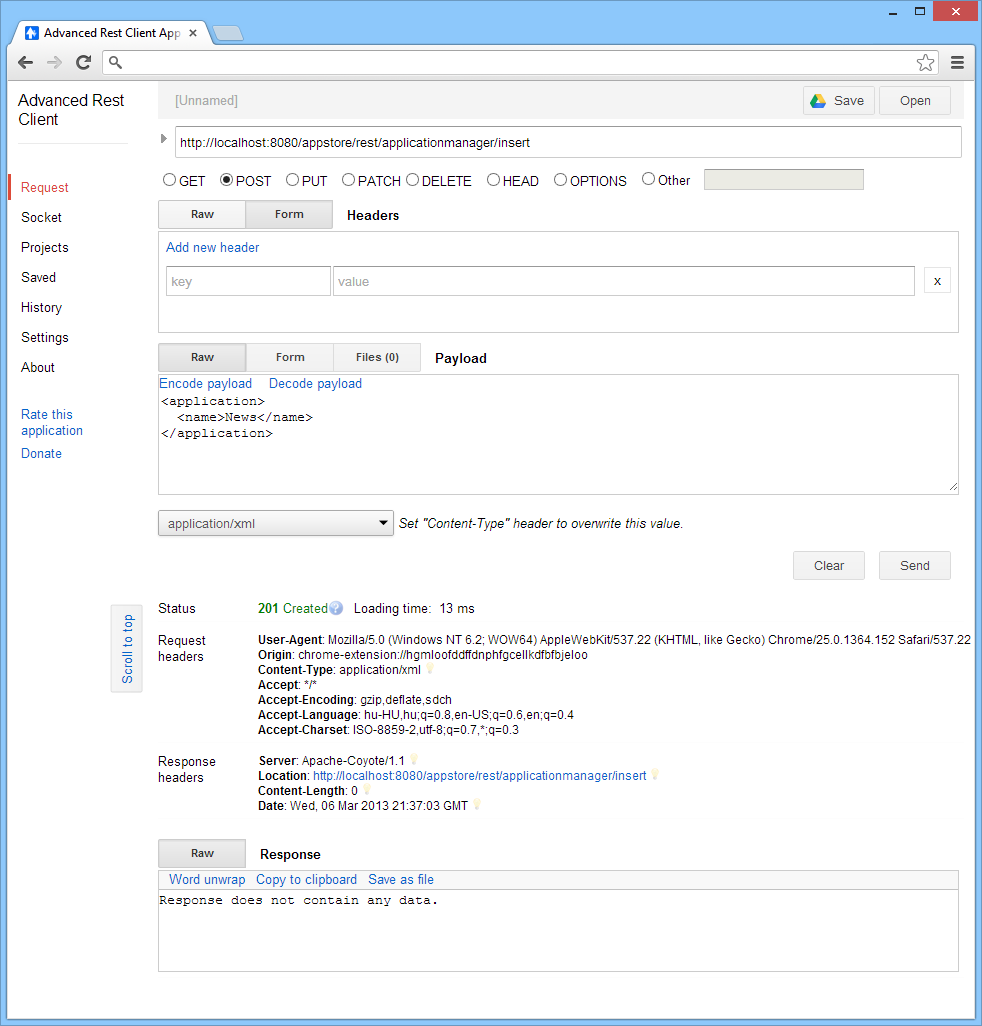
\includegraphics{img/web_services/rest_client_1.png}
\caption{A POST operation with an XML payload on the application store}
\end{figure}

\begin{figure}[htbp]
\centering
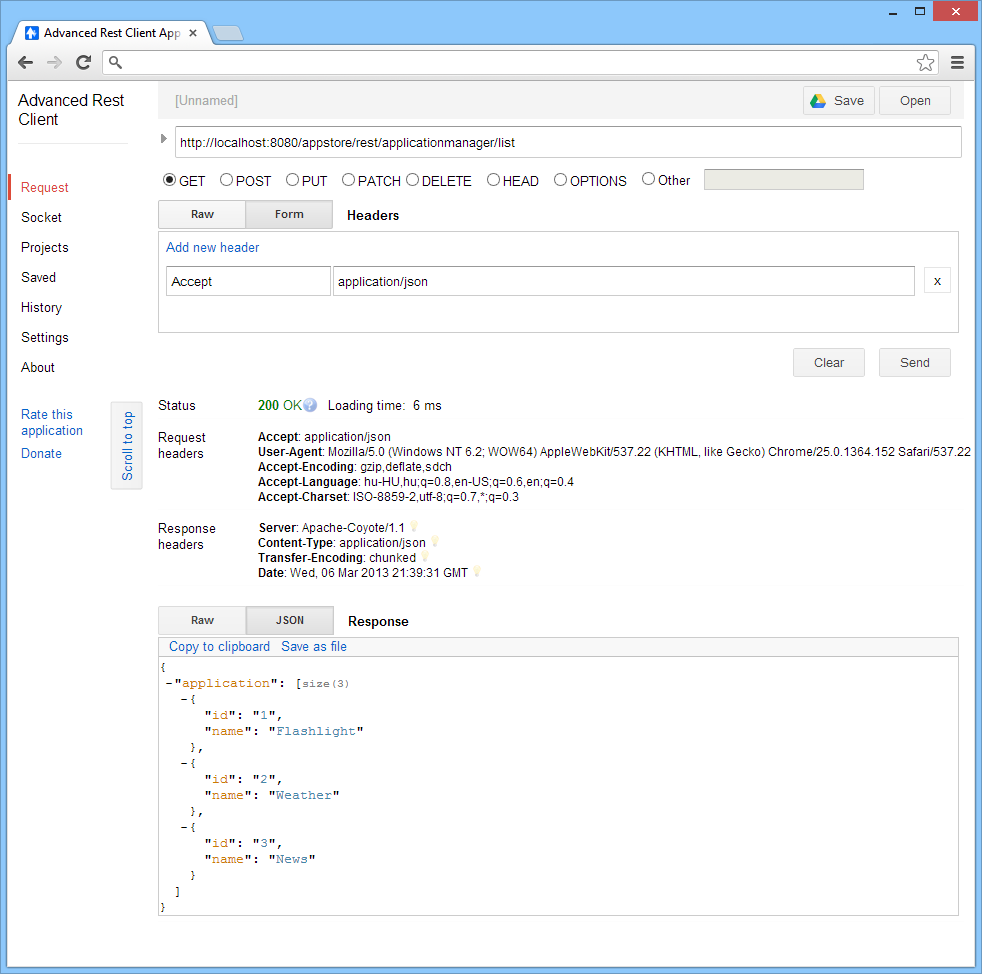
\includegraphics{img/web_services/rest_client_2.png}
\caption{A GET operation on the application store returning JSON}
\end{figure}

\section{Google App Engine}

From Wikipedia (\url{http://en.wikipedia.org/wiki/Google_App_Engine}):
,,Google App Engine is a platform as a service (PaaS) cloud computing
platform for developing and hosting web applications in Google-managed
data centers. Applications are sandboxed and run across multiple
servers. App Engine offers automatic scaling for web applications---as
the number of requests increases for an application, App Engine
automatically allocates more resources for the web application to handle
the additional demand. Google App Engine is free up to a certain level
of consumed resources.''

\section{Tips and troubleshooting}

\begin{itemize}
\itemsep1pt\parskip0pt\parsep0pt
\item
  You can show the \textbf{Show Servers} view by clicking \textbf{Window
  \textbar{} Show View \textbar{} Other\ldots{}} and choosing
  \textbf{Server \textbar{} Servers}.
\item
  You can display the internal web browser by clicking \textbf{Window
  \textbar{} Show View \textbar{} Other\ldots{}} and choosing
  \textbf{General \textbar{} Internal Web Browser}.
\item
  If error are displayed because the \texttt{javax} packages cannot be
  found, right click on the project name, click \textbf{Properties} and
  look into \textbf{Targeted Runtimes}. It's also worth trying to clean
  the project.
\item
  Sometime Maven does not download the dependencies and the project's
  \textbf{Maven Dependencies} node is empty. Right click the project and
  choose \textbf{Run As \textbar{} Maven install}. Because Maven depends
  on the accessibility of it's main repository, this might not work for
  the first time: try again, it might does.
\end{itemize}

\section{Additional materials}

\subsection{Creating a JSP Servlet}

\url{http://www.vogella.com/articles/EclipseWTP/article.html}

\begin{enumerate}
\def\labelenumi{\arabic{enumi}.}
\item
  Start Eclipse.
\item
  Click \textbf{File \textbar{} New \textbar{} Other}. Pick \textbf{Web
  \textbar{} Dynamic Web Project}. Set the project name to
  \texttt{hu.bme.mit.inf.helloworld}.
\item
  Right click on the \texttt{hu.bme.mit.inf.mdsd.helloworld} project's
  name: pick \textbf{New \textbar{} Other\ldots{}} and choose
  \textbf{Web \textbar{} Servlet}. Set the Java package to
  \texttt{hu.bme.mit.inf.helloworld} and the Class name to
  \texttt{HelloWorld}.
\item
  While observing the possible settings, click \textbf{Next},
  \textbf{Next}, \textbf{Finish}.
\item
  Add the following code to the \texttt{doGet} method in the
  \texttt{HelloWorld} class:

\begin{Shaded}
\begin{Highlighting}[]
\KeywordTok{protected} \DataTypeTok{void} \FunctionTok{doGet}\NormalTok{(HttpServletRequest request, HttpServletResponse response) }
  \KeywordTok{throws} \NormalTok{ServletException, IOException \{}
  \NormalTok{response.}\FunctionTok{setContentType}\NormalTok{(}\StringTok{"text/plain"}\NormalTok{);}
  \NormalTok{PrintWriter out = response.}\FunctionTok{getWriter}\NormalTok{();}
  \NormalTok{out.}\FunctionTok{println}\NormalTok{(}\StringTok{"Hello world."}\NormalTok{);}
\NormalTok{\}}
\end{Highlighting}
\end{Shaded}

  Choose \textbf{Manually define a new server} and set the
  \textbf{Server runtime environment} to the previously created
  \texttt{MDSD Tomcat}. Click \textbf{Next} and \textbf{Finish}.

  A browser tab will appear with the address
  \url{http://localhost:8080/hu.bme.mit.inf.helloworld/HelloWorld} and
  will display the following content (formatted as plain text):

\begin{verbatim}
Hello world.
\end{verbatim}
\item
  Modify the code, e.g.~change \texttt{Hello world} to
  \texttt{Hello worlds}. Eclipse will build the project automatically
  and deploy it on the Tomcat server. The \textbf{Console} view shows
  the following log:

\begin{verbatim}
INFO: Reloading Context with name [/hu.bme.mit.inf.helloworld] is completed
\end{verbatim}
\item
  Refresh the browser's page to see if it worked.
\end{enumerate}

\section{Sources}

\begin{itemize}
\itemsep1pt\parskip0pt\parsep0pt
\item
  Creating Bottom-Up Web Service,
  \url{http://wiki.eclipse.org/Creating_a_Bottom-Up_Java_Web_Service}
\item
  JSON and REST, The New Kids on the Data Block,
  \url{http://www.slideshare.net/rmaclean/json-and-rest}
\item
  Build a RESTful Web service using Jersey and Apache Tomcat:
  \url{http://www.ibm.com/developerworks/library/wa-aj-tomcat/}
\end{itemize}

\chapter{Yakindu}

From Wikipedia
(\url{http://en.wikipedia.org/wiki/YAKINDU_Statechart_Tools}): Yakindu
(\url{http://statecharts.org/}) Statechart Tools (SCT) is an open source
tool for the specification and development of reactive, event-driven
systems with the help of state machines. It consists of an easy-to-use
tool for graphical editing and provides validation, simulation and code
generators for different target platforms. The users come from both the
industrial and academic sectors.''

\begin{figure}[htbp]
\centering

\includegraphics{img/yakindu/yakindu_logo.png}
\caption{The logo of Yakindu}
\end{figure}

Yakindu is developed by itemis, the same company that created Xtext.

\begin{figure}[htbp]
\centering

\includegraphics{img/yakindu/itemis_logo.png}
\caption{The logo of itemis}
\end{figure}

\section{Prerequisites}

From the Yakindu update site, install the following plug-ins for
Eclipse:

\begin{itemize}
\itemsep1pt\parskip0pt\parsep0pt
\item
  Yakindu SCT 2
\item
  Copy Paste Patch
\item
  YAKINDU SCT Generator C
\item
  YAKINDU SCT Generator Java
\item
  Yakindu Statechart Tools (SCT) 2
\item
  Yakindu Statechart Tools (SCT) 2 SDK
\end{itemize}

\section{Modeling}

\begin{enumerate}
\def\labelenumi{\arabic{enumi}.}
\item
  Create a new \textbf{YAKINDU Xpand Generator Project}.
\item
  Add a new \textbf{YAKINDU Statechart Model}.
\item
  Add the following code to the editor:

\begin{verbatim}
interface Service:
in event request
in event read
var success : boolean

internal:
event complete
\end{verbatim}
\item
  Create the statechart \#1 as shown on the figure.

  \begin{figure}[htbp]
  \centering
  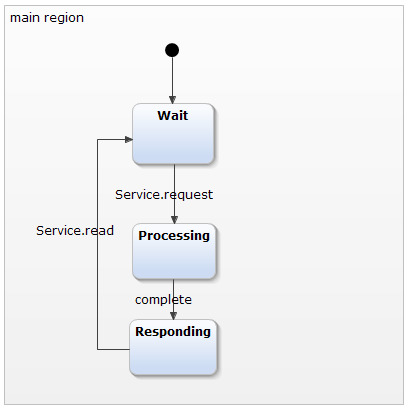
\includegraphics{img/yakindu/statechart_1.png}
  \caption{Statechart \#1}
  \end{figure}
\item
  Run the statechart (\textbf{Run As \textbar{} YAKINDU Statechart}) and
  experiment with the \textbf{Simulation View}.
\item
  Extend your statechart to \#2 by adding a new \textbf{State} and a
  \textbf{Choice}. Keep in mind that the transitions have priorities,
  which may cause them to behave differently than expected.

  You can edit the \textbf{Transition Priority} in the \textbf{Choice}'s
  \textbf{Properties} view (Right click the \textbf{Choice} on the
  canvas and pick \textbf{Show Properties View}).

  \begin{figure}[htbp]
  \centering
  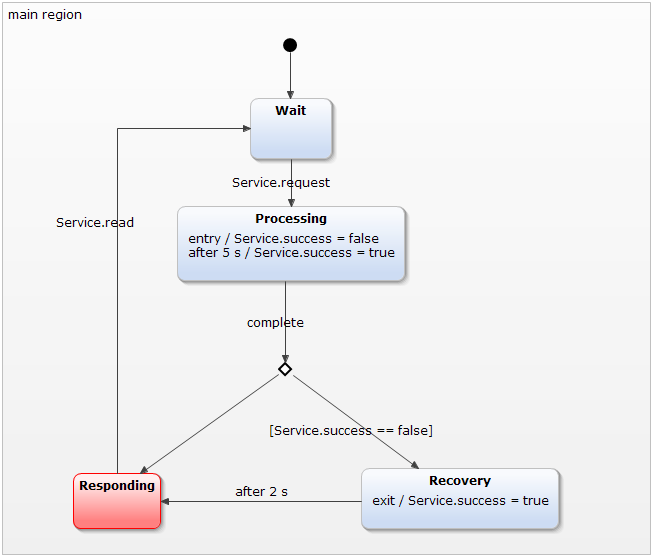
\includegraphics{img/yakindu/statechart_2.png}
  \caption{Statechart \#2}
  \end{figure}
\item
  Extend your statechart to \#3 by adding a new \textbf{Composite State}
  called \texttt{Frontend}.

  \begin{figure}[htbp]
  \centering
  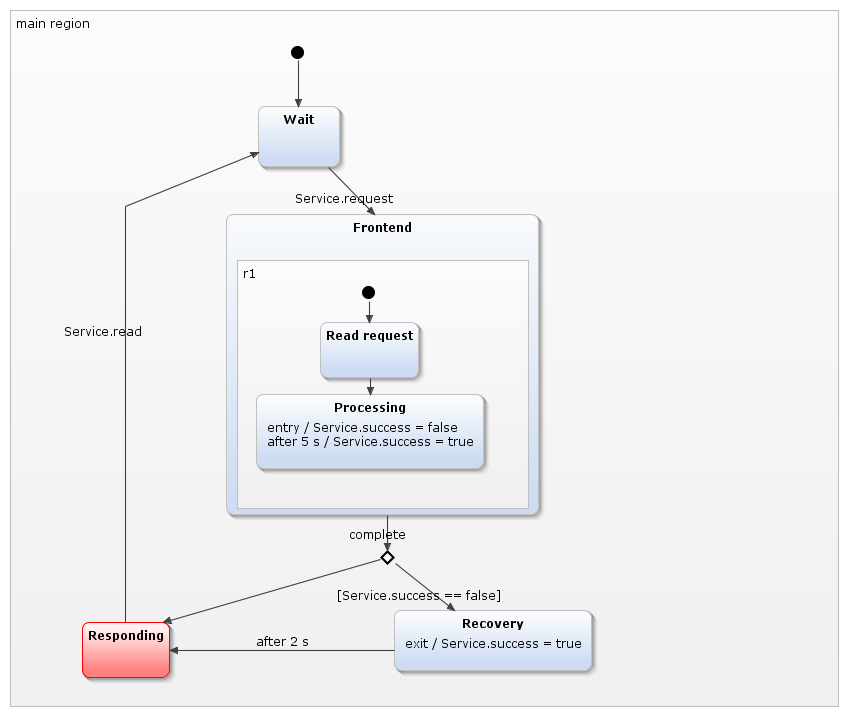
\includegraphics{img/yakindu/statechart_3.png}
  \caption{Statechart \#3}
  \end{figure}
\item
  Modify the statechart definition block to the following:

\begin{verbatim}
interface Service:
in event request
in event read
var success : boolean

internal:
event complete
event execute
event finish

interface DB:
in event access
in event response
var data: integer 
\end{verbatim}
\item
  Using the new events, extend your statechart to \#4 by adding a new
  \textbf{Composite State} called \texttt{Database}.

  \begin{figure}[htbp]
  \centering
  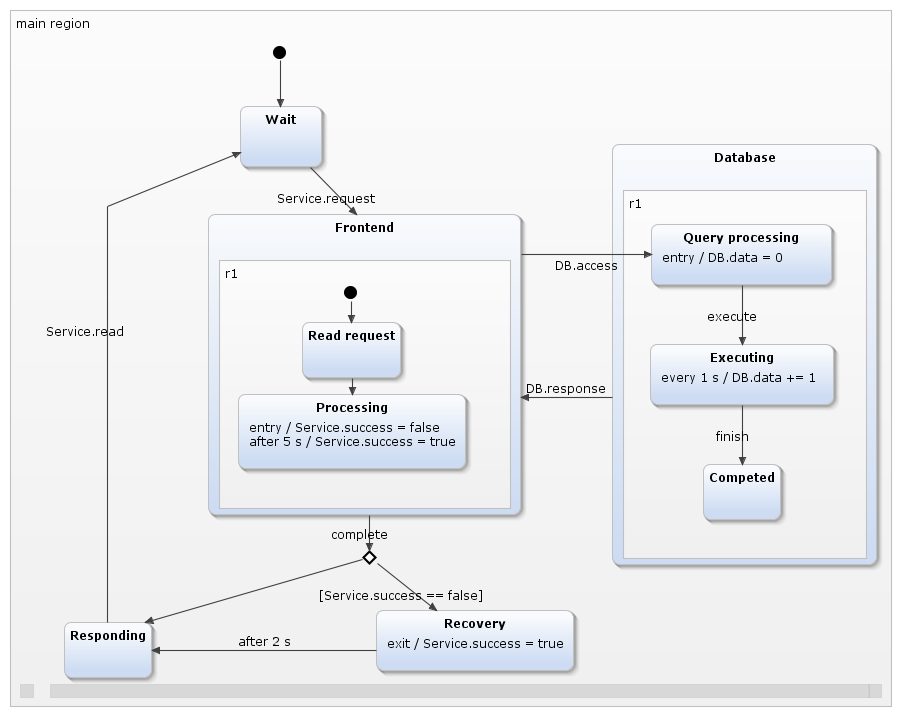
\includegraphics{img/yakindu/statechart_4.png}
  \caption{Statechart \#4}
  \end{figure}
\item
  Modify your statechart to get \#5 by adding a new \textbf{Shallow
  History} to the \texttt{Frontend} state.

  \begin{figure}[htbp]
  \centering
  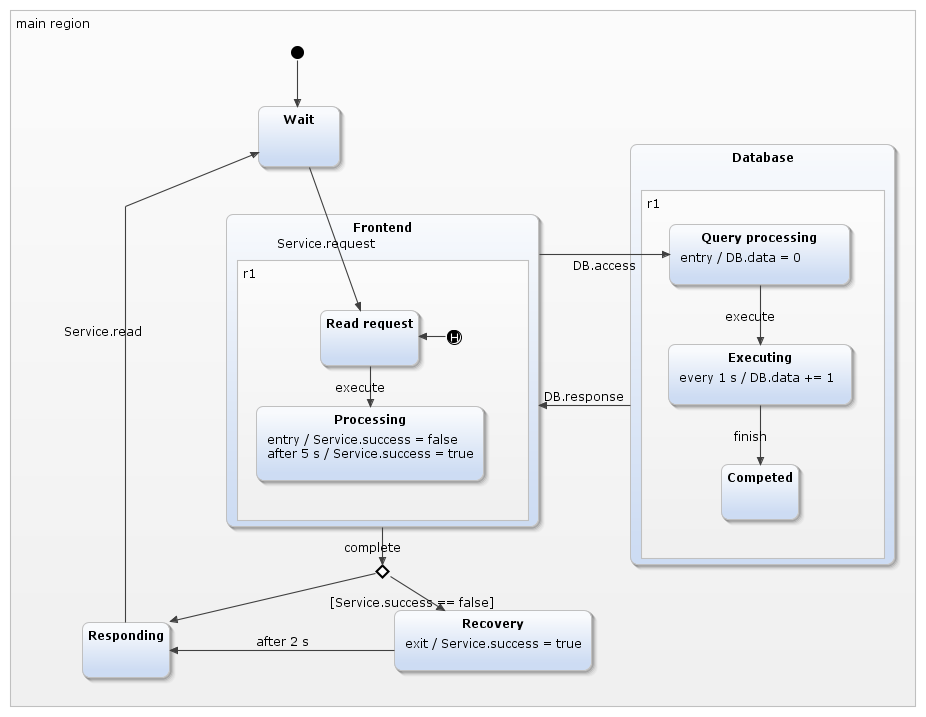
\includegraphics{img/yakindu/statechart_5.png}
  \caption{Statechart \#5}
  \end{figure}
\end{enumerate}

\section{Code generation}

\begin{enumerate}
\def\labelenumi{\arabic{enumi}.}
\item
  Add a generator by clicking \textbf{File \textbar{} New \textbar{}
  Other\ldots{}} and picking \textbf{Yakindu Statechart Generator
  Model}. Name it \texttt{service.sgen}, choose \textbf{YAKINDU SCT Java
  Code Generator} and tick the \texttt{service.sct} statechart.
\item
  Modify the \texttt{service.sgen} file to the following:

\begin{verbatim}
GeneratorModel for yakindu::java {

  statechart service {
    feature Outlet {
      targetProject = "yakindu.labor"
      targetFolder = "src-gen"
    }

    feature GeneralFeatures {
      TimerService = true
    }
  }

}
\end{verbatim}
\item
  Add the \texttt{src-gen} folder to the \textbf{Build Path}.
\item
  Create a class named \texttt{ServiceClient} in the \texttt{src} folder
  in a package named \texttt{service}:

\begin{Shaded}
\begin{Highlighting}[]
\KeywordTok{package service;}

\KeywordTok{import org.yakindu.scr.TimerService;}
\KeywordTok{import org.yakindu.scr.service.ServiceStatemachine;}
\KeywordTok{import org.yakindu.scr.service.ServiceStatemachine.State;}

\KeywordTok{public} \KeywordTok{class} \NormalTok{ServiceClient \{}

  \KeywordTok{public} \DataTypeTok{static} \DataTypeTok{void} \FunctionTok{main}\NormalTok{(String[] args) }\KeywordTok{throws} \NormalTok{InterruptedException \{}
    \NormalTok{ServiceStatemachine sm = }\KeywordTok{new} \FunctionTok{ServiceStatemachine}\NormalTok{();}
    \NormalTok{sm.}\FunctionTok{setTimerService}\NormalTok{(}\KeywordTok{new} \FunctionTok{TimerService}\NormalTok{());}

    \NormalTok{sm.}\FunctionTok{enter}\NormalTok{();}

    \NormalTok{sm.}\FunctionTok{getSCIService}\NormalTok{().}\FunctionTok{raiseRequest}\NormalTok{();}
    \NormalTok{sm.}\FunctionTok{runCycle}\NormalTok{();}

    \KeywordTok{if} \NormalTok{(sm.}\FunctionTok{isStateActive}\NormalTok{(State.}\FunctionTok{main_region_Frontend_r1_Read_request}\NormalTok{)) \{}
      \NormalTok{System.}\FunctionTok{out}\NormalTok{.}\FunctionTok{println}\NormalTok{(}\StringTok{"Reading request."}\NormalTok{);}
    \NormalTok{\}}
  \NormalTok{\}}

\NormalTok{\}}
\end{Highlighting}
\end{Shaded}
\item
  Run the program. It will produce the following output:

\begin{verbatim}
Reading request.
\end{verbatim}
\item
  Create a method that runs a number of cycles, each of which sleeps for
  0.2 seconds and then notifies the statechart.

\begin{Shaded}
\begin{Highlighting}[]
\KeywordTok{private} \DataTypeTok{static} \DataTypeTok{void} \FunctionTok{sleep}\NormalTok{(ServiceStatemachine sm, }\DataTypeTok{int} \NormalTok{limit)}
    \KeywordTok{throws} \NormalTok{InterruptedException \{}
  \KeywordTok{for} \NormalTok{(}\DataTypeTok{int} \NormalTok{i = }\DecValTok{0}\NormalTok{; i < limit; i++) \{}
    \NormalTok{Thread.}\FunctionTok{sleep}\NormalTok{(}\DecValTok{200}\NormalTok{);}
    \NormalTok{sm.}\FunctionTok{runCycle}\NormalTok{();}
  \NormalTok{\}}
\NormalTok{\}}
\end{Highlighting}
\end{Shaded}
\item
  Add the following call to the \texttt{main} method:

\begin{Shaded}
\begin{Highlighting}[]
\NormalTok{sm.}\FunctionTok{getSCICommon}\NormalTok{().}\FunctionTok{raiseExecute}\NormalTok{();}
\end{Highlighting}
\end{Shaded}
\item
  This will cause a compile-time error. The problem is that the
  \texttt{execute} event is internal, therefore the
  \texttt{raiseExecute()} method is private and cannot be accessed from
  the \texttt{main} method. To address this, create a new interfaced
  called \texttt{Common} for the the internal events.

\begin{verbatim}
interface Common:
in event complete
in event execute
in event finish
\end{verbatim}
\item
  Modify your statechart's transitions accodingly to get statechart \#6.

  \begin{figure}[htbp]
  \centering
  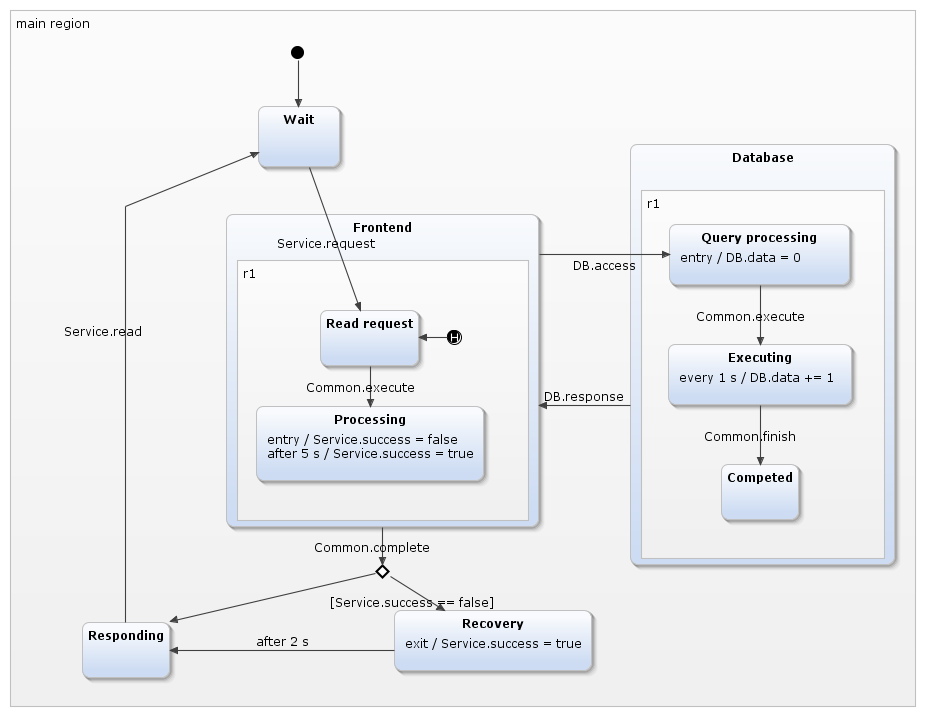
\includegraphics{img/yakindu/statechart_6.png}
  \caption{Statechart \#6}
  \end{figure}
\item
  After this, the \texttt{raiseExecute()} will be visible. Continue
  expanding the \texttt{main} method with the following:

\begin{Shaded}
\begin{Highlighting}[]
\NormalTok{sm.}\FunctionTok{getSCICommon}\NormalTok{().}\FunctionTok{raiseExecute}\NormalTok{(); }\CommentTok{// we added this previously}

\NormalTok{sm.}\FunctionTok{getSCIDB}\NormalTok{().}\FunctionTok{raiseAccess}\NormalTok{();}
\NormalTok{sm.}\FunctionTok{runCycle}\NormalTok{();}

\NormalTok{sm.}\FunctionTok{getSCICommon}\NormalTok{().}\FunctionTok{raiseExecute}\NormalTok{();}
\NormalTok{sm.}\FunctionTok{runCycle}\NormalTok{();}

\FunctionTok{sleep}\NormalTok{(sm, }\DecValTok{30}\NormalTok{);}

\NormalTok{sm.}\FunctionTok{getSCIDB}\NormalTok{().}\FunctionTok{raiseResponse}\NormalTok{();}
\NormalTok{sm.}\FunctionTok{runCycle}\NormalTok{();}

\NormalTok{System.}\FunctionTok{out}\NormalTok{.}\FunctionTok{println}\NormalTok{(}\StringTok{"Data = "} \NormalTok{+ sm.}\FunctionTok{getSCIDB}\NormalTok{().}\FunctionTok{getData}\NormalTok{());}

\FunctionTok{sleep}\NormalTok{(sm, }\DecValTok{10}\NormalTok{);}
\NormalTok{sm.}\FunctionTok{getSCICommon}\NormalTok{().}\FunctionTok{raiseComplete}\NormalTok{();}
\NormalTok{sm.}\FunctionTok{runCycle}\NormalTok{();}

\KeywordTok{if} \NormalTok{(!sm.}\FunctionTok{getSCIService}\NormalTok{().}\FunctionTok{getSuccess}\NormalTok{()) \{}
  \NormalTok{System.}\FunctionTok{out}\NormalTok{.}\FunctionTok{println}\NormalTok{(}\StringTok{"Unsuccessful call."}\NormalTok{);}
  \NormalTok{System.}\FunctionTok{out}\NormalTok{.}\FunctionTok{println}\NormalTok{(}\StringTok{"Recovery state active: "} \NormalTok{+ }
    \NormalTok{sm.}\FunctionTok{isStateActive}\NormalTok{(State.}\FunctionTok{main_region_Recovery}\NormalTok{) + }\StringTok{"."}\NormalTok{);}
  \FunctionTok{sleep}\NormalTok{(sm, }\DecValTok{11}\NormalTok{); }\CommentTok{// more than 2 seconds}
\NormalTok{\}}

\KeywordTok{if} \NormalTok{(sm.}\FunctionTok{isStateActive}\NormalTok{(State.}\FunctionTok{main_region_Responding}\NormalTok{)) \{}
  \NormalTok{System.}\FunctionTok{out}\NormalTok{.}\FunctionTok{println}\NormalTok{(}\StringTok{"Responding."}\NormalTok{);}
\NormalTok{\}}

\NormalTok{sm.}\FunctionTok{exit}\NormalTok{();}
\end{Highlighting}
\end{Shaded}
\item
  Run the application. The output is the following:

\begin{verbatim}
Reading request.
Data = 6
Unsuccessful call.
Recovery state active: true.
Responding.
\end{verbatim}

  If you run the program multiple times, you can observe that the
  \texttt{Data} value is sometimes 5 instead of 6. Think about reason
  behind this.
\end{enumerate}

\section{Tips}

\begin{itemize}
\itemsep1pt\parskip0pt\parsep0pt
\item
  If the Java code is not generated automatically, right click the
  \texttt{service.sgen} file and click \textbf{Generate Statechart
  Artifacts}.
\item
  If you cannot find the \textbf{Simulation View}, right click the
  \textbf{SC Simulation} perspective's name and choose \textbf{Reset}.
\end{itemize}

\chapter{Bonita}

Source code snippets and URLs are available at
\url{https://svn.inf.mit.bme.hu/edu/trunk/mdsd/handout/public/bonita_connector_materials/}.

\section{Introduction}

\begin{enumerate}
\def\labelenumi{\arabic{enumi}.}
\item
  Start the Bonita Studio and choose ``MyProcessDiagram (1.0)'' process.
\item
  We have changed the browse workflow a bit: it serve as an application
  collection that can be browsed or extended from various sources.
\item
  Start the workflow and inspect it: at this page the application
  available in our database should be displayed. Currently this list is
  empty.
\item
  There are buttons in the lower part of the page that shows the
  available options of extension sources. Those sources are services.
  Select the WebService option and go to the next page.
\item
  The \textbf{New apps} page displays the newly downloaded pages. Those
  applications will be inserted to the database. If you click next the
  first page will be displayed. At the end of the lecture this list will
  show the newly inserted applications too.
\item
  Choose \textbf{None} and end the workflow.
\end{enumerate}

\section{Scripting Reminder}

\begin{enumerate}
\def\labelenumi{\arabic{enumi}.}
\item
  At first substitute the web service with a script on ``Update by web
  service'': \texttt{{[}"New"{]}}.
\item
  This list should be directed to the newApplications variable, and
  replacing it.
\end{enumerate}

\section{Database Integration}

\begin{enumerate}
\def\labelenumi{\arabic{enumi}.}
\item
  Lets integrate our workflow with a MySQL database. Start the MySQL
  Workbench 5.2 CE.
\item
  Choose the SQL development section and select the Local MySQL
  database.
\item
  A dolphin in an aquarium will authenticate you: the password is
  \texttt{root}.
\item
  An SQL development environment will appear. We have created a database
  for the workflow: select the application table in the applications
  database, \textbf{right click \textbar{} Select Rows - Limit 1000}.
\item
  The query and the result will appear with the single application
  called \texttt{EvilStore}.
\item
  Our applications will be saved to this table. This query will be
  copied to the workflow, so do not close it.
\item
  Select the Load the application names task and add a connector:
  \textbf{Database \textbar{} MySQL}. Name it to
  \texttt{ApplicationQuery} and fill out the form as described in the
  picture below.

  \begin{figure}[htbp]
  \centering
  \includegraphics{img/bonita_connector/database_config.png}
  \caption{Bonita db connector configuration}
  \end{figure}
\item
  Fill the \textbf{Query} field in the next page:

\begin{Shaded}
\begin{Highlighting}[]
\KeywordTok{SELECT} \NormalTok{* }\KeywordTok{FROM} \NormalTok{applications.application}
\end{Highlighting}
\end{Shaded}
\item
  Click \textbf{Test configuration}:

  \begin{figure}[htbp]
  \centering
  \includegraphics{img/bonita_connector/database_test.png}
  \caption{Bonita db test}
  \end{figure}
\item
  Direct the values of the \texttt{rowset} to the Applications variable
  (\texttt{java rowSet.getValues()}). Select the replace strategy.
\item
  Now write the insert script in the ``Save to DB'' task. Add a new
  MySQL connector to the task, fill it in the same way.
\item
  Write the script as a return value of a method:

\begin{Shaded}
\begin{Highlighting}[]
\NormalTok{String ret =}
  \StringTok{"INSERT INTO `applications`.`application` "}\NormalTok{+}
  \StringTok{"(`Name`) VALUES "}
\DataTypeTok{boolean} \NormalTok{hasItem = }\KeywordTok{false}
\KeywordTok{for}\NormalTok{(item in newApplications) \{}
  \KeywordTok{if}\NormalTok{(hasItem) ret+=}\StringTok{","}
  \NormalTok{ret+=}\StringTok{"('"}\NormalTok{+item.}\FunctionTok{replaceAll}\NormalTok{(}\StringTok{"[}\CharTok{\textbackslash{}\textbackslash{}}\StringTok{W]"}\NormalTok{, }\StringTok{""}\NormalTok{)+}\StringTok{"')"}
  \NormalTok{hasItem = }\KeywordTok{true}
\NormalTok{\}}
\KeywordTok{return} \NormalTok{ret}
\end{Highlighting}
\end{Shaded}
\item
  Test it with the evaluate button. The result will be (explain why):

\begin{Shaded}
\begin{Highlighting}[]
\KeywordTok{INSERT} \KeywordTok{INTO} \NormalTok{`applications`.`application` (`Name`) }\KeywordTok{VALUES} \NormalTok{(}\StringTok{'O'}\NormalTok{),(}\StringTok{'b'}\NormalTok{),(}\StringTok{'j'}\NormalTok{),(}\StringTok{'e'}\NormalTok{),(}\StringTok{'c'}\NormalTok{),(}\StringTok{'t'}\NormalTok{)}
\end{Highlighting}
\end{Shaded}
\item
  Run the workflow, the result should be inserted to the table.

  \begin{figure}[htbp]
  \centering
  \includegraphics{img/bonita_connector/database_insert.png}
  \caption{Bonita db test}
  \end{figure}
\end{enumerate}

\section{Web services}

You can start the Tomcat server with the \texttt{start-tomcat.bat} batch
file on the Desktop. The
\texttt{C:\textbackslash{}tomcat\textbackslash{}webapps} files are
deployed

On the Tomcat server, you have web applications available: a JAX-WS SOA
web service and a JAX-RS REST web service.

You have to web services available. Both offer the same functionality:
they generate an arbitrary number of \texttt{Application} objects.

\subsection{SOA web service}

To test the SOA web service, start Google Chrome's Advanced REST Client
plug-in. Set the URL to
\url{http://localhost:8080/appstore-ws/services/ApplicationManager} and
the HTTP method to \textbf{POST}. Add a header field \texttt{SOAPAction}
(with an empty value) to the \textbf{Headers}. Paste the following code
to the \textbf{Payload} field.

\begin{Shaded}
\begin{Highlighting}[]
\KeywordTok{<?xml} \NormalTok{version="1.0" encoding="UTF-8" standalone="no"}\KeywordTok{?>}
\KeywordTok{<soapenv:Envelope}\OtherTok{ xmlns:soapenv=}\StringTok{"http://schemas.xmlsoap.org/soap/envelope/"} 
\OtherTok{  xmlns:xsd=}\StringTok{"http://www.w3.org/2001/XMLSchema"} 
\OtherTok{  xmlns:xsi=}\StringTok{"http://www.w3.org/2001/XMLSchema-instance"}\KeywordTok{>}
  \KeywordTok{<soapenv:Body>}
    \KeywordTok{<generateApplications}\OtherTok{ xmlns=}\StringTok{"http://ws.server.appstore.inf.mit.bme.hu"}\KeywordTok{>}
      \KeywordTok{<count>}\NormalTok{20}\KeywordTok{</count>}
    \KeywordTok{</generateApplications>}
  \KeywordTok{</soapenv:Body>}
\KeywordTok{</soapenv:Envelope>}
\end{Highlighting}
\end{Shaded}

\emph{Notes:} we can generate the SOA envelope with the Eclipse WTP
platform. If you generate the client (as seen in the \emph{web service
laboratory}), you can observe the SOA envelope in the TCP/IP monitor.

\begin{figure}[htbp]
\centering
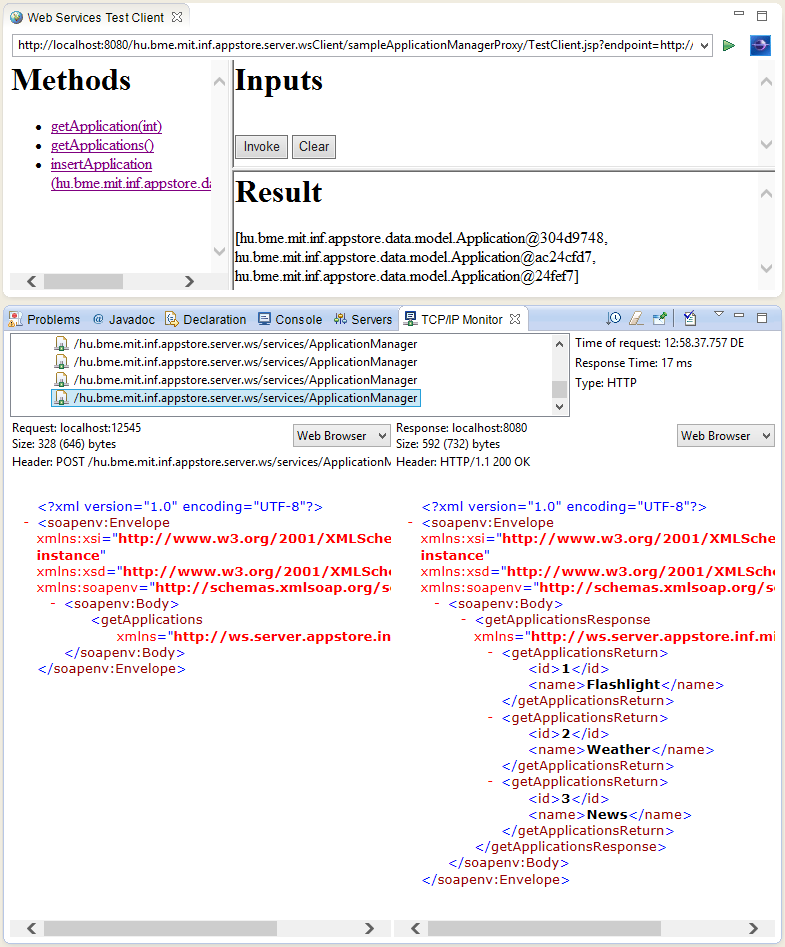
\includegraphics{img/web_services/tcp_ip_monitor_list.png}
\caption{The SOA envelope can be observed in the TCP/IP monitor}
\end{figure}

\begin{figure}[htbp]
\centering
\includegraphics{img/bonita_connector/ws.png}
\caption{SOA web service}
\end{figure}

\subsubsection{SoapUI}

SoapUI (\url{http://www.soapui.org/}) is capable of generating SOA
envelopes from the WSDL file.

Just create a \textbf{New soapUI Project}, add the
\texttt{ApplicationManager.wsdl} WSDL file as \textbf{Initial
WSDL/WADL}. Tick \textbf{Create Request} and click \textbf{OK}. The SOA
envelope will be generated.

\begin{figure}[htbp]
\centering
\includegraphics{img/bonita_connector/soapui.png}
\caption{SOA web service}
\end{figure}

\url{http://www-inf.int-evry.fr/cours/WebServices/TP_Workflow/publish_news.html}

\subsection{REST web service}

To observe the REST web service, simply visit
\url{http://localhost:8080/appstore-rest/rest/applicationmanager/generate/20}.

\begin{figure}[htbp]
\centering
\includegraphics{img/bonita_connector/rest.png}
\caption{REST web service}
\end{figure}

\begin{itemize}
\itemsep1pt\parskip0pt\parsep0pt
\item
  Target NS:
  \texttt{http://localhost:8080/appstore-ws/services/ApplicationManager}
\item
  Service name: \texttt{ApplicationManagerService}
\item
  Port name: \texttt{ApplicationManager}
\item
  Request: same XML as above.
\item
  End point address: as above,
  \texttt{http://localhost:8080/appstore-ws/services/ApplicationManager}
\item
  Binding: \texttt{http://schemas.xmlsoap.org/wsdl/soap/}
\end{itemize}

\begin{figure}[htbp]
\centering
\includegraphics{img/bonita_connector/web_service_client.png}
\caption{\textbf{Web Service Client} dialog}
\end{figure}

Write the following code:

\begin{Shaded}
\begin{Highlighting}[]
\KeywordTok{import javax.xml.transform.dom.DOMSource;}

\NormalTok{def output = (DOMSource) response}
\NormalTok{def ret = []}
\NormalTok{def apps =}
   \NormalTok{output.}\FunctionTok{getNode}\NormalTok{().}
   \NormalTok{childNodes.}\FunctionTok{item}\NormalTok{(}\DecValTok{0}\NormalTok{).}
   \NormalTok{childNodes.}\FunctionTok{item}\NormalTok{(}\DecValTok{1}\NormalTok{).}
   \NormalTok{childNodes.}\FunctionTok{item}\NormalTok{(}\DecValTok{0}\NormalTok{).}
   \NormalTok{childNodes}

\KeywordTok{for}\NormalTok{(}\DataTypeTok{int} \NormalTok{i=}\DecValTok{0}\NormalTok{; i<apps.}\FunctionTok{length}\NormalTok{; i++)\{}
   \NormalTok{ret.}\FunctionTok{add}\NormalTok{(apps.}\FunctionTok{item}\NormalTok{(i).}\FunctionTok{textContent}\NormalTok{)}
\NormalTok{\}}
\KeywordTok{return} \NormalTok{ret}
\end{Highlighting}
\end{Shaded}

\section{Creating a new connector}

\begin{enumerate}
\def\labelenumi{\arabic{enumi}.}
\item
  Go to \textbf{Connectors \textbar{} New Connector}, and name it to
  \texttt{MyRestConnectorForApplications}.
\item
  Add an output parameter named \texttt{result} with \texttt{List} type.
\item
  Write the following Java code:

\begin{Shaded}
\begin{Highlighting}[]
\KeywordTok{import java.util.ArrayList;}
\KeywordTok{import java.util.List;}

\KeywordTok{import org.ow2.bonita.connector.core.ConnectorError;}
\KeywordTok{import org.ow2.bonita.connector.core.ProcessConnector;}

\KeywordTok{public} \KeywordTok{class} \NormalTok{MyRestConnectorForApplications }\KeywordTok{extends} \NormalTok{ProcessConnector \{}

  \KeywordTok{private} \NormalTok{ArrayList<String> results;}

  \FunctionTok{@Override}
  \KeywordTok{protected} \DataTypeTok{void} \FunctionTok{executeConnector}\NormalTok{() }\KeywordTok{throws} \NormalTok{Exception \{}
    \NormalTok{results = }\KeywordTok{new} \NormalTok{ArrayList<String>();}
    \NormalTok{results.}\FunctionTok{add}\NormalTok{(}\StringTok{"A"}\NormalTok{);}
    \NormalTok{results.}\FunctionTok{add}\NormalTok{(}\StringTok{"B"}\NormalTok{);}
  \NormalTok{\}}

  \FunctionTok{@Override}
  \KeywordTok{protected} \NormalTok{List<ConnectorError> }\FunctionTok{validateValues}\NormalTok{() \{}
    \CommentTok{// TODO Auto-generated method stub}
    \KeywordTok{return} \KeywordTok{null}\NormalTok{;}
  \NormalTok{\}}

  \CommentTok{/**}
\CommentTok{   * Getter for output argument 'result'}
\CommentTok{   * DO NOT REMOVE NOR RENAME THIS GETTER, }
\CommentTok{   * unless you also change the related entry in the XML descriptor file}
\CommentTok{   */}
  \KeywordTok{public} \NormalTok{java.}\FunctionTok{util}\NormalTok{.}\FunctionTok{ArrayList} \FunctionTok{getResult}\NormalTok{() \{}
    \KeywordTok{return} \NormalTok{results;}
  \NormalTok{\}}
\NormalTok{\}}
\end{Highlighting}
\end{Shaded}
\item
  Put it into the workflow, use \textbf{replace} strategy.
\item
  Edit the code to get the following:

\begin{Shaded}
\begin{Highlighting}[]
\KeywordTok{import java.io.InputStream;}
\KeywordTok{import java.net.URL;}
\KeywordTok{import java.net.URLConnection;}
\KeywordTok{import java.util.ArrayList;}
\KeywordTok{import java.util.List;}

\KeywordTok{import org.ow2.bonita.connector.core.ConnectorError;}
\KeywordTok{import org.ow2.bonita.connector.core.ProcessConnector;}

\KeywordTok{import javax.xml.parsers.DocumentBuilder;}
\KeywordTok{import javax.xml.parsers.DocumentBuilderFactory;}

\KeywordTok{import org.w3c.dom.Document;}
\KeywordTok{import org.w3c.dom.Node;}
\KeywordTok{import org.w3c.dom.NodeList;}

\KeywordTok{public} \KeywordTok{class} \NormalTok{MyRestConnectorForApplications }\KeywordTok{extends} \NormalTok{ProcessConnector \{}

  \KeywordTok{private} \NormalTok{ArrayList<String> results;}

  \FunctionTok{@Override}
  \KeywordTok{protected} \DataTypeTok{void} \FunctionTok{executeConnector}\NormalTok{() }\KeywordTok{throws} \NormalTok{Exception \{}

    \NormalTok{URL url = }\KeywordTok{new} \NormalTok{URL(}\StringTok{"http://localhost:8080/appstore-rest/rest/applicationmanager/generate/3"}\NormalTok{);}
    \NormalTok{URLConnection connection = url.}\FunctionTok{openConnection}\NormalTok{();}
    \NormalTok{Document document = }\FunctionTok{parseXmlDom}\NormalTok{(connection.}\FunctionTok{getInputStream}\NormalTok{());}

    \NormalTok{results = }\KeywordTok{new} \NormalTok{ArrayList<String>();}
    \NormalTok{NodeList apps = document.}\FunctionTok{getElementsByTagName}\NormalTok{(}\StringTok{"applications"}\NormalTok{).}\FunctionTok{item}\NormalTok{(}\DecValTok{0}\NormalTok{).}\FunctionTok{getChildNodes}\NormalTok{();}
    \KeywordTok{for}\NormalTok{(}\DataTypeTok{int} \NormalTok{i = }\DecValTok{0}\NormalTok{; i< apps.}\FunctionTok{getLength}\NormalTok{(); i++) \{}
      \NormalTok{results.}\FunctionTok{add}\NormalTok{(apps.}\FunctionTok{item}\NormalTok{(i).}\FunctionTok{getTextContent}\NormalTok{());}
    \NormalTok{\}}
  \NormalTok{\}}
  \KeywordTok{public} \DataTypeTok{static} \NormalTok{Document }\FunctionTok{parseXmlDom}\NormalTok{(InputStream is) \{}

    \NormalTok{Document document = }\KeywordTok{null}\NormalTok{;}
    \KeywordTok{try} \NormalTok{\{}

      \CommentTok{// getting the default implementation of DOM builder}
      \NormalTok{DocumentBuilderFactory dbf = DocumentBuilderFactory.}\FunctionTok{newInstance}\NormalTok{();}

      \NormalTok{dbf.}\FunctionTok{setValidating}\NormalTok{(}\KeywordTok{false}\NormalTok{);}
      \NormalTok{dbf.}\FunctionTok{setIgnoringComments}\NormalTok{(}\KeywordTok{true}\NormalTok{);}
      \NormalTok{dbf.}\FunctionTok{setIgnoringElementContentWhitespace}\NormalTok{(}\KeywordTok{true}\NormalTok{);}
      \NormalTok{dbf.}\FunctionTok{setNamespaceAware}\NormalTok{(}\KeywordTok{true}\NormalTok{);}

      \NormalTok{DocumentBuilder builder = dbf.}\FunctionTok{newDocumentBuilder}\NormalTok{();}

      \CommentTok{// parsing the XML file}
      \NormalTok{document = builder.}\FunctionTok{parse}\NormalTok{(is);}

    \NormalTok{\} }\KeywordTok{catch} \NormalTok{(Exception e) \{}
      \CommentTok{// catching all exceptions}
      \NormalTok{System.}\FunctionTok{out}\NormalTok{.}\FunctionTok{println}\NormalTok{(e.}\FunctionTok{toString}\NormalTok{());}
    \NormalTok{\}}
    \KeywordTok{return} \NormalTok{document;}
  \NormalTok{\}}

  \FunctionTok{@Override}
  \KeywordTok{protected} \NormalTok{List<ConnectorError> }\FunctionTok{validateValues}\NormalTok{() \{}
    \CommentTok{// TODO Auto-generated method stub}
    \KeywordTok{return} \KeywordTok{null}\NormalTok{;}
  \NormalTok{\}}

  \CommentTok{/**}
\CommentTok{   * Getter for output argument 'result'}
\CommentTok{   * DO NOT REMOVE NOR RENAME THIS GETTER, }
\CommentTok{   * unless you also change the related entry in the XML descriptor file}
\CommentTok{   */}
  \KeywordTok{public} \NormalTok{java.}\FunctionTok{util}\NormalTok{.}\FunctionTok{ArrayList} \FunctionTok{getResult}\NormalTok{() \{}
    \KeywordTok{return} \NormalTok{results;}
  \NormalTok{\}}
\NormalTok{\}}
\end{Highlighting}
\end{Shaded}
\end{enumerate}

\chapter{Introduction to the Eclipse Modeling Framework}

Author: Oszkár Semeráth

\section{About the EMF}

From Wikipedia
(\url{http://en.wikipedia.org/wiki/Eclipse_Modeling_Framework})
,,Eclipse Modeling Framework (EMF) is an Eclipse-based modeling
framework and code generation facility for building tools and other
applications based on a structured data model.'' EMF's data model is
lightweight as it only defines a few but well-defined modeling elements.
However, it has an extensive tooling support and community. For example,
you can define the textual or graphical syntax of a language and
generate the appropriate editors.

EMF can generate Java code from the model with only a click of a button.
The generated code is capable of serialisation to XMI and
deserialisation from XMI files.

EMF home page: \url{http://www.eclipse.org/modeling/emf/}

\section{Description of the task}

The goal of this exercise is to create the metamodel a customized
Entity-Relationship Diagrams (ERD). Those diagrams can aid the
development of software components that working with complex data
structures. A later exercise will show you how can complete database
schemes, full classes and the automated mapping between those can be
derived from these documents.

The following image presents an example of Entity Relation diagram.

\begin{figure}[htbp]
\centering
\includegraphics{img/emf/ERD1.png}
\caption{Example of an Entity-Relationship diagram}
\end{figure}

\section{Prerequisites}

The Eclipse Modeling Tools edition contains every required plug-in.

\section{Ecore model: step-by-step}

\begin{enumerate}
\def\labelenumi{\arabic{enumi}.}
\item
  Create a new \textbf{Empty EMF Project} by \textbf{File \textbar{} New
  \textbar{} Other\ldots{} \textbar{} Eclipse Modeling Framework
  \textbar{} Empty EMF Project}. Name it to
  \texttt{hu.bme.mit.mdsd.erdiagram}.
\item
  There is a folder in the project named \textbf{model}. Create a new
  \textbf{ECore Model} in it by right click to the folder \textbar{} New
  \textbar{} Other\ldots{} \textbar{} ECore Model. Name it to
  \texttt{ERDiagram.ecore}.
\item
  A new editor opens that shows that the model resource has a yet
  unnamed empty package. Fill the missing properties in the property
  view:

  \begin{itemize}
  \itemsep1pt\parskip0pt\parsep0pt
  \item
    Ns Prefix: \texttt{hu.bme.mit.mdsd.erdiagram}
  \item
    Ns URI: \texttt{hu.bme.mit.mdsd.erdiagram}
  \end{itemize}

  To show unavailable view go to \textbf{Window \textbar{} Show View
  \textbar{} Other\ldots{} \textbar{} General}.
\item
  It is possible to create the model in this tree editor but there is a
  more convenient editor for this purpose. Right click to the ecore file
  and choose the \textbf{Initialize ECore diagram File\ldots{}} option.
  Name it to \textbf{ERDiagram.ecorediag}.
\item
  Let's make the following part:

  \begin{figure}[htbp]
  \centering
  \includegraphics{img/emf/ERDiagram00.png}
  \caption{A very simple Ecore model with two \texttt{EClass}es and an
  \texttt{EReference} between them}
  \end{figure}

  The features should be presented:

  \begin{itemize}
  \itemsep1pt\parskip0pt\parsep0pt
  \item
    \texttt{EClass} (with \textbf{Is Abstract} property)
  \item
    \texttt{EReference} (with multiplicities and \textbf{Is
    Containment})
  \item
    \texttt{Inheritance} between the classes.
  \end{itemize}

  The objects of the instance models of the metamodel have to be in a
  tree hiearcy with respect of the composition references. The editor
  can validate the model.

  \begin{itemize}
  \itemsep1pt\parskip0pt\parsep0pt
  \item
    \textbf{Advanced Options:} Direct editing for the properties of the
    elements of the model.
  \end{itemize}
\item
  The result can be observed in the \textbf{Outline} view. Note that
  deleting from model and the diagram are different things. Create the
  metamodel of the Entity Relation Diagram on your own like it was a
  class diagram. A possible result is:

  \begin{figure}[htbp]
  \centering
  \includegraphics{img/emf/ERDiagram01.png}
  \caption{The metamodel of the ER diagram}
  \end{figure}

  The \texttt{EOpposite} feature should be presented.
\item
  Adding attributes to the model. Showing the \texttt{EEnum}.

  \begin{figure}[htbp]
  \centering
  \includegraphics{img/emf/ERDiagram02.png}
  \caption{The metamodel completed with \texttt{EAttributes}}
  \end{figure}

  The difference between the \texttt{EAttribute} and \texttt{EReference}
  is that the EAttribute is referring to an \texttt{EDataTypes} opposed
  to \texttt{EReferences} that endings to \texttt{EClasses}.

  The metamodel lacks of \texttt{EOperations}. The semantic of those is
  that they are functions over the model elements like refactoring. The
  EMF is a lightweight modelling tool with heavy support for data
  modelling, but little for operations. Instead of this use manager
  classes to write methods.

  At this phase we have all visible details of the Entity Relation
  Diagrams.
\item
  Adding namespace to the diagram, this could be the name of the
  diagram. The types of the attributes should be defined outside of the
  model, and referred by the diagram.

  \begin{figure}[htbp]
  \centering
  \includegraphics{img/emf/ERDiagram03.png}
  \caption{The model with the \texttt{AttributeType} class and the
  \texttt{namespace} attribute}
  \end{figure}
\item
  The diagram may refer to an existing database with existing tables.
  The referred table and column names might be described in the diagram
  (for example the \texttt{User} entity is stored in the
  \texttt{USER\_TABLE} because its name is reserved). Note the multiple
  inheritance at the \texttt{Attribute} entity.

  \begin{figure}[htbp]
  \centering
  \includegraphics{img/emf/ERDiagram04.png}
  \caption{The model now supports the connection to databases}
  \end{figure}
\end{enumerate}

\section{Editor: step-by-step}

This example shows how to generate classes and an editor from Ecore
models.

\begin{enumerate}
\def\labelenumi{\arabic{enumi}.}
\item
  The ecore files are the blueprints of the domain specific languages.
  To use the tooling support available in Eclipse some kind of Java
  class representation of those ``boxes'' are needed. Fortunately those
  classes can be automatically generated.

  Right click the ecore file and \textbf{New \textbar{} Other \textbar{}
  Eclipse Modeling Framework \textbar{} EMF Generator Model}. The
  default \texttt{ERDiagram.genmodel} is fine. At the next step choose
  that the generator generate from an Ecore model. In the third step the
  URI of the Ecore model have to be added. Click on load and next.
  Choose the only avaliable package to generate and hit finish.
\item
  Another tree editor opens similar to the ecore editor. Browse some of
  the setting in the property editor. Right click to the root, and
  choose the \textbf{Generate Model} command. Three package has been
  generated in the source folder. Browse for example the
  \texttt{hu.bme.mit.mdsd.erdiagram/src/ERDiagram/EntityRelationDiagram.java}
  file, and you can see that nothing strange has been generated. The
  implementation class has some unusual field, but the implementations
  of the functions of the interface are quite simple.
\item
  Generate an \textbf{editor}. Right click to the root of the genmodel
  file, and generate edit and editor in this order.
\item
  Right click to the project, and choose \textbf{Run as \textbar{}
  Eclipse} application.
\item
  Create an empty project by \textbf{File \textbar{} New \textbar{}
  Other\ldots{} \textbar{} General \textbar{} Project} and name it to
  \textbf{Diagrams}.
\item
  Create a new Entity Relation Diagram into the new project by right
  clicking on it and picking \textbf{New \textbar{} Other \textbar{}
  Example EMF Model Creation Wizard \textbar{} ERDiagram Model}. The
  name can be the default \texttt{My.erdiagram}, and the model object
  (what we want to edit) should be \textbf{Entity Relation Diagram}.
\item
  Create the instance model. The editor is quite self-explanatory to
  use.
\end{enumerate}

\begin{figure}[htbp]
\centering
\includegraphics{img/emf/ERDInstance.png}
\caption{The tree editor for the Ecore model}
\end{figure}

\section{Model manipulation: step-by-step}

The following example shows how to edit the model from code.

\begin{enumerate}
\def\labelenumi{\arabic{enumi}.}
\item
  Create a new \textbf{Plug-in Project} by right click \textbar{} New
  \textbar{} Plug-in Project. Name it to
  \texttt{hu.bme.mit.mdsd.erdiagrammanipulator}.
\item
  Add the following dependencies:

  \begin{longtable}[c]{@{}ll@{}}
  \hline\noalign{\medskip}
  \texttt{hu.bme.mit.mdsd.erdiagram} & The edited domain.
  \\\noalign{\medskip}
  \texttt{org.eclipse.emf.ecore.xmi} & The instance model is serialised
  as an XMI document.
  \\\noalign{\medskip}
  \hline
  \end{longtable}
\item
  Create a class to the source folder:

  \begin{longtable}[c]{@{}ll@{}}
  \hline\noalign{\medskip}
  package & \texttt{hu.bme.mit.jpadatamodelmanipulator}
  \\\noalign{\medskip}
  name & \texttt{ModelEditor}
  \\\noalign{\medskip}
  \hline
  \end{longtable}
\item
  Create an initialisation method for model loading.

\begin{Shaded}
\begin{Highlighting}[]
\KeywordTok{public} \DataTypeTok{void} \FunctionTok{init}\NormalTok{() \{}
   \CommentTok{// For the initialisation of the model.}
   \CommentTok{// Without this the following error happens:}
   \CommentTok{//  "Package with uri 'hu.bme.mit.mdsd.erdiagram' not found."}
   \NormalTok{ERDiagramPackage.}\FunctionTok{eINSTANCE}\NormalTok{.}\FunctionTok{eClass}\NormalTok{();}

   \CommentTok{// Defining that the files with the .erdiagram extension should be parsed as an xmi.}
   \NormalTok{Resource.}\FunctionTok{Factory}\NormalTok{.}\FunctionTok{Registry} \NormalTok{reg = Resource.}\FunctionTok{Factory}\NormalTok{.}\FunctionTok{Registry}\NormalTok{.}\FunctionTok{INSTANCE}\NormalTok{;}
   \NormalTok{reg.}\FunctionTok{getExtensionToFactoryMap}\NormalTok{().}\FunctionTok{put}\NormalTok{(}\StringTok{"erdiagram"}\NormalTok{, }\KeywordTok{new} \FunctionTok{XMIResourceFactoryImpl}\NormalTok{());}
\NormalTok{\}}
\end{Highlighting}
\end{Shaded}
\item
  The model is in an xmi file that can be generally handled as a
  resource. A resource can be referenced by an URI. Write a method that
  loads a resource:

\begin{Shaded}
\begin{Highlighting}[]
\KeywordTok{public} \NormalTok{Resource }\FunctionTok{getResourceFromURI}\NormalTok{(URI uri) \{}
   \NormalTok{ResourceSet resSet = }\KeywordTok{new} \FunctionTok{ResourceSetImpl}\NormalTok{();}
   \NormalTok{Resource resource = resSet.}\FunctionTok{getResource}\NormalTok{(uri, }\KeywordTok{true}\NormalTok{);}
   \KeywordTok{return} \NormalTok{resource;}
\NormalTok{\}}
\end{Highlighting}
\end{Shaded}
\item
  The resource simply can be saved:

\begin{Shaded}
\begin{Highlighting}[]
\KeywordTok{public} \DataTypeTok{void} \FunctionTok{saveResource}\NormalTok{(Resource resource) \{}
   \KeywordTok{try} \NormalTok{\{}
     \NormalTok{resource.}\FunctionTok{save}\NormalTok{(Collections.}\FunctionTok{EMPTY_MAP}\NormalTok{);}
   \NormalTok{\} }\KeywordTok{catch} \NormalTok{(IOException e) \{}
      \NormalTok{System.}\FunctionTok{out}\NormalTok{.}\FunctionTok{println}\NormalTok{(}\StringTok{"The following error occured during saving the resource: "}
        \NormalTok{+ e.}\FunctionTok{getMessage}\NormalTok{());}
   \NormalTok{\}}
\NormalTok{\}}
\end{Highlighting}
\end{Shaded}
\item
  The content of the resource should be the ED diagram object.

\begin{Shaded}
\begin{Highlighting}[]
\KeywordTok{public} \NormalTok{EntityRelationDiagram }\FunctionTok{getModelFromResource}\NormalTok{(Resource resource) \{}
   \CommentTok{// check the content!}
   \NormalTok{EntityRelationDiagram root = (EntityRelationDiagram) resource.}\FunctionTok{getContents}\NormalTok{().}\FunctionTok{get}\NormalTok{(}\DecValTok{0}\NormalTok{);}
   \KeywordTok{return} \NormalTok{root;}
\NormalTok{\}}
\end{Highlighting}
\end{Shaded}
\item
  The ER diagram object should be edited through the interface and
  instantinated by the generated factory methods. This method creates a
  custom table data object for every entity that doesn't already have
  one:

\begin{Shaded}
\begin{Highlighting}[]
\KeywordTok{public} \DataTypeTok{void} \FunctionTok{editDiagram}\NormalTok{(EntityRelationDiagram diagram) \{}
   \KeywordTok{for}\NormalTok{(Entity entity : diagram.}\FunctionTok{getEntities}\NormalTok{()) \{}
      \KeywordTok{if}\NormalTok{(entity.}\FunctionTok{getCustomTable}\NormalTok{() == }\KeywordTok{null}\NormalTok{) \{}
         \NormalTok{TableData tableData = ERDiagramFactory.}\FunctionTok{eINSTANCE}\NormalTok{.}\FunctionTok{createTableData}\NormalTok{();}
         \NormalTok{tableData.}\FunctionTok{setTableName}\NormalTok{(entity.}\FunctionTok{getName}\NormalTok{().}\FunctionTok{toUpperCase}\NormalTok{()+}\StringTok{"_TABLE"}\NormalTok{);}
         \NormalTok{entity.}\FunctionTok{setCustomTable}\NormalTok{(tableData);}
      \NormalTok{\}}
   \NormalTok{\}}
\NormalTok{\}}
\end{Highlighting}
\end{Shaded}

  The result can be printed to the output by this method:

\begin{Shaded}
\begin{Highlighting}[]
\KeywordTok{public} \DataTypeTok{void} \FunctionTok{printTables}\NormalTok{(EntityRelationDiagram diagram) \{}
   \KeywordTok{for}\NormalTok{(Entity entity : diagram.}\FunctionTok{getEntities}\NormalTok{()) \{}
      \NormalTok{System.}\FunctionTok{out}\NormalTok{.}\FunctionTok{println}\NormalTok{(entity.}\FunctionTok{getCustomTable}\NormalTok{().}\FunctionTok{getTableName}\NormalTok{());}
   \NormalTok{\}}
\NormalTok{\}}
\end{Highlighting}
\end{Shaded}
\item
  You can get the URI by right click \textbar{} \textbf{Properties} and
  copy the file to a string. For example my URI is:

\begin{Shaded}
\begin{Highlighting}[]
\NormalTok{URI uri = URI.}\FunctionTok{createFileURI}\NormalTok{(}\StringTok{"C:/workspace/Diagrams/My.erdiagram"}\NormalTok{);}
\end{Highlighting}
\end{Shaded}

  The main method looks like:

\begin{Shaded}
\begin{Highlighting}[]
\KeywordTok{public} \DataTypeTok{static} \DataTypeTok{void} \FunctionTok{main}\NormalTok{(String[] args) \{}
   \NormalTok{ModelEditor editor = }\KeywordTok{new} \FunctionTok{ModelEditor}\NormalTok{();}
   \NormalTok{editor.}\FunctionTok{init}\NormalTok{();}
   \NormalTok{URI uri = URI.}\FunctionTok{createFileURI}\NormalTok{(}\StringTok{"C:/workspace/Diagrams/My.erdiagram"}\NormalTok{);}
   \NormalTok{Resource resource = editor.}\FunctionTok{getResourceFromURI}\NormalTok{(uri);}
   \NormalTok{EntityRelationDiagram diagram = editor.}\FunctionTok{getModelFromResource}\NormalTok{(resource);}
   \NormalTok{editor.}\FunctionTok{editDiagram}\NormalTok{(diagram);}
   \NormalTok{editor.}\FunctionTok{printTables}\NormalTok{(diagram);}
   \NormalTok{editor.}\FunctionTok{saveResource}\NormalTok{(resource);}
\NormalTok{\}}
\end{Highlighting}
\end{Shaded}

  Right click to the class and choose \textbf{Run as \textbar{} Java
  Application}. This will run our code as a simple Java application that
  loads modifes and saves a model.
\end{enumerate}

\section{Summary}

At the end the following steps have been made:

\begin{figure}[htbp]
\centering
\includegraphics{img/emf/ERD2.png}
\caption{The workflow of the laboratory and the dependencies between the
artifacts (marked with dashed lines)}
\end{figure}

The final metamodel is:

\begin{figure}[htbp]
\centering
\includegraphics{img/emf/ERDiagram05_final.png}
\caption{The final Ecore model}
\end{figure}

\section{General tips}

\begin{itemize}
\itemsep1pt\parskip0pt\parsep0pt
\item
  If anything goes wrong with the regeneration and there is problem with
  your code you have two options:

  \begin{itemize}
  \itemsep1pt\parskip0pt\parsep0pt
  \item
    If the document was not edited by hand or it isn't valuable delete
    it. Generate the code again, and it should be fine. It works on the
    Manifest.MF and the plugin.xml too.
  \item
    In other case don't be afraid of rewriting. For example if you
    delete an item from the metamodel the xmi that contains the instance
    model might have remaining tags with undefined type. That makes the
    xmi invalid, but it isn't necessary to start over the instance
    model; simply delete the unwanted part from the code by hand.
  \end{itemize}
\end{itemize}

\chapter{Code generation technologies}

\section{JVM based languages}

\textbf{Summary:}
\url{http://en.wikipedia.org/wiki/List_of_JVM_languages}

Beyond Java, many programming languages exist which are capable of
producing software that can run on the Java Virtual Machine (JVM). These
languages can usually feature close interoperability with Java
libraries: call their methods and accept their calls.

In recent years, the TIOBE index
(\url{http://www.tiobe.com/index.php/content/paperinfo/tpci/index.html}),
which shows the popularity of programming languages put Java in the top
two positions, while Scala, Groovy and Clojure was in the top 100.

\subsection{Scala}

\textbf{Home page:} \url{http://www.scala-lang.org/}

Like Java, Scala is strongly object-oriented and statically typed but
also uses elements from functional programming. Scala natively supports
building concurrent applications.

\begin{figure}[htbp]
\centering
\includegraphics{img/code_generation/scala_logo.png}
\caption{The logo of Scala}
\end{figure}

\subsection{Groovy}

\textbf{Home page:} \url{http://groovy.codehaus.org/}

Groovy is a script-like language with functional elements. Most
syntactically correct Java code is also a corrent Groovy code. Groovy
supports both static and dynamis typing.

\textbf{Remark:} in Bonita (\url{http://www.bonitasoft.com/}), used on
the Service Integration course, you can specify expressions in Groovy
(\url{http://www.bonitasoft.com/resources/documentation/groovy}).

\begin{figure}[htbp]
\centering
\includegraphics{img/code_generation/groovy_logo.png}
\caption{The logo of Groovy}
\end{figure}

\subsection{Clojure}

\textbf{Home page:} \url{http://clojure.org/}

Clojure is a dialect of the Lisp programming language. Software created
in Clojure can be compiled to run on the JVM, the .NET Common Language
Runtime (CLR) or a JavaScript engine. Clojure is a functional language
which strongly support building concurrent applications.

\begin{figure}[htbp]
\centering
\includegraphics{img/code_generation/clojure_logo.png}
\caption{The logo of Clojure}
\end{figure}

\section{Code generation with Eclipse technologies}

\subsection{Xtext}

\textbf{Home page:} \url{http://www.eclipse.org/Xtext/}

Xtext is a framework creating programming languages and domain-specific
languages. Xtext is capable of generating the parser the interpreter and
provide Eclipse IDE support for the language. The developers task is to
define language's grammar in \texttt{.xtext} files
(\url{http://www.eclipse.org/Xtext/documentation.html\#_1}). Xtext's
components build on the Eclipse Modeling Framework (EMF), so Xtext
development can be easily integrated with other EMF based technologies
(e.g.~GMF).

\begin{figure}[htbp]
\centering
\includegraphics{img/code_generation/xtext_logo.png}
\caption{The logo of Xtext}
\end{figure}

\subsection{Xbase}

\textbf{Home page:} \url{http://wiki.eclipse.org/Xbase}

Xbase is partial programming language. It's purpose is to serve as a
basis of the expessions in the programming languages generated by Xtext.
Xbase expressions closely resemble Java expressions: the mutual elements
include strings, if and foreach structures, method invocations,
constructors, etc.

The target platform of Xbase expressions is the JVM. At first, Xbase
generates Java code and later compiles it to byte code.

Xbase is statically typed. It's features include closures and operator
overloading. It provides convenient type inference mechanism and a
switch structure more advanced than Java's (see the Xbase home page
above).

\textbf{Remark:} the \texttt{check} expression in IncQuery patterns
(\url{http://viatra.inf.mit.bme.hu/incquery}) are written in Xbase.

\begin{figure}[htbp]
\centering
\includegraphics{img/code_generation/xbase_logo.png}
\caption{The logo of Xbase}
\end{figure}

\subsection{Xpand}

\textbf{Home page:}
\url{http://www.eclipse.org/modeling/m2t/?project=xpand},
\url{http://wiki.eclipse.org/Xpand}

Xpand is a highly specialised language, with the purpose of generating
code from EMF models. Xpand is statically typed and support polymorphic
template invocation, aspect-oriented programming (AOP), model
transformation, model validation, etc.

Example code:
\url{http://www.openarchitectureware.org/pub/documentation/4.3.1/html/contents/emf_tutorial.html\#emf_tutorial_generating_code}

\subsubsection{Xtend (deprecated)}

\textbf{Home page:} \url{http://wiki.eclipse.org/Xpand/Galileo}

See also:
\url{http://dslmeinte.wordpress.com/2011/09/19/using-xtexts-xtend2-language/}

Originally, Xtend was a sublanguage of Xpand (file with \texttt{.ext}
and \texttt{.xpt} extension). It was capable of supporting functional
programming elements.

\textbf{Remark:} Xpand and its Xtend technologies are no longer actively
developed, so we don't use it in the courses.

\subsection{Xtend (previously called Xtend2)}

\textbf{Home page:} \url{http://www.eclipse.org/xtend/}

Blog post:
\url{http://blog.efftinge.de/2010/12/xtend-2-successor-to-xpand.html}

Wikipedia:
\url{http://en.wikipedia.org/wiki/Xtend_(programming_language)}

Xtend2 was created with the intent to replace Xpand and Xtend. Later the
number ,,2'`was dropped from its name. Hence, when we use the term
,,Xtend'' we refer to the new technology. In order to be
distinguishable, the files created with the newer Xtend technology have
the extension \texttt{.xtend}.

Xtend is a JVM based language. It's grammar and editor was created with
Xtext. The language uses Xbase expressions. Xtend is statically typed,
and uses both object-oriented and functional elements -- e.g.~lambda
expressions.

Xtend can cover the whole process of generating code from an EMF model,
including the definition of the templates and imperative code that
executes the process.

\begin{figure}[htbp]
\centering
\includegraphics{img/code_generation/xtend_logo.png}
\caption{The logo of Xtend}
\end{figure}

\chapter{JPA}

This tutorial shows a simple example that covers most of the JPA
technology.

\begin{enumerate}
\def\labelenumi{\arabic{enumi}.}
\item
  Create a new java project with the name
  \texttt{hu.bme.mit.mdsd.jpaexample}.
\item
  Create a new package to the \textbf{src} folder and name it to
  \texttt{car.entities.handwritten}.
\item
  Create a class named \texttt{Dealer}:

\begin{Shaded}
\begin{Highlighting}[]
\KeywordTok{public} \KeywordTok{class} \NormalTok{Dealer \{}
  \KeywordTok{private} \NormalTok{String name;}
  \KeywordTok{private} \NormalTok{List<Producer> productRange = }\KeywordTok{new} \NormalTok{ArrayList<Producer>();}
\NormalTok{\}}
\end{Highlighting}
\end{Shaded}
\item
  And a one named \texttt{Producer}:

\begin{Shaded}
\begin{Highlighting}[]
\KeywordTok{public} \KeywordTok{class} \NormalTok{Producer \{}
  \KeywordTok{private} \NormalTok{String name;}
  \KeywordTok{private} \NormalTok{List<Dealer> worksWith = }\KeywordTok{new} \NormalTok{ArrayList<Dealer>();}
\NormalTok{\}}
\end{Highlighting}
\end{Shaded}
\item
  Generate the getters and setters.
\item
  To persist the instances to a database some jar file is needed:

  \begin{itemize}
  \itemsep1pt\parskip0pt\parsep0pt
  \item
    \textbf{javax.persistence\_2.0.4.jar:} The java persistence API
    itself.
  \item
    \textbf{eclipselink.jar:} The way of object-relational mapping is
    defined in this jar. We use Eclipse link at this lecture.
  \item
    \textbf{mysql-connector-java-5.1.22-bin.jar:} The database driver.
    In this case the application is connected to a MySQL database.
  \end{itemize}

  Those jar files can be downloaded from the site of the vendor.
\item
  Those files should be added to the project. Previously the Maven tool
  is used for this purpose, but at this case they will be added
  manually. Create a new folder to the project and call it to
  \texttt{lib}. Put the files to this folder by drag and drop them.
\item
  Those files should be added to the classpath of the project. To do
  this right click to the project and choose \textbf{Build Path
  \textbar{} Configure Build Path}. Add the jars to the build path with
  the \textbf{Add JARs} button at the Lybraries menu.
\item
  Some configuration is inevitable. Create a \texttt{META-INF} folder
  into the project and add a file into it named
  \texttt{persistence.xml}. The content:

\begin{Shaded}
\begin{Highlighting}[]
\KeywordTok{<?xml} \NormalTok{version="1.0" encoding="UTF-8"}\KeywordTok{?>}
\KeywordTok{<persistence}\OtherTok{ version=}\StringTok{"2.0"}
\OtherTok{  xmlns=}\StringTok{"http://java.sun.com/xml/ns/persistence"}
\OtherTok{  xmlns:xsi=}\StringTok{"http://www.w3.org/2001/XMLSchema-instance"}
\OtherTok{  xsi:schemaLocation=}\StringTok{"http://java.sun.com/xml/ns/persistence http://java.sun.com/xml/ns/persistence/persistence_2_0.xsd"}\KeywordTok{>}
  \KeywordTok{<persistence-unit}\OtherTok{ name=}\StringTok{"cars"}\KeywordTok{>}
    \KeywordTok{<exclude-unlisted-classes>}\NormalTok{false}\KeywordTok{</exclude-unlisted-classes>}
    \KeywordTok{<properties>}
      \KeywordTok{<property}\OtherTok{ name=}\StringTok{"javax.persistence.jdbc.password"}\OtherTok{ value=}\StringTok{"root"}\KeywordTok{/>}
      \KeywordTok{<property}\OtherTok{ name=}\StringTok{"javax.persistence.jdbc.user"}\OtherTok{ value=}\StringTok{"root"}\KeywordTok{/>}
      \KeywordTok{<property}\OtherTok{ name=}\StringTok{"javax.persistence.jdbc.driver"}\OtherTok{ value=}\StringTok{"com.mysql.jdbc.Driver"}\KeywordTok{/>}
      \KeywordTok{<property}\OtherTok{ name=}\StringTok{"javax.persistence.jdbc.url"}\OtherTok{ value=}\StringTok{"jdbc:mysql://localhost:3306/test"}\KeywordTok{/>}
      \KeywordTok{<property}\OtherTok{ name=}\StringTok{"eclipselink.ddl-generation"}\OtherTok{ value=}\StringTok{"create-tables"}\KeywordTok{/>}
      \KeywordTok{<property}\OtherTok{ name=}\StringTok{"eclipselink.logging.level"}\OtherTok{ value=}\StringTok{"INFO"}\KeywordTok{/>}
    \KeywordTok{</properties>}
  \KeywordTok{</persistence-unit>}
\KeywordTok{</persistence>}
\end{Highlighting}
\end{Shaded}

  This configuration defines the following properties:

  \begin{itemize}
  \itemsep1pt\parskip0pt\parsep0pt
  \item
    A name for the persistence-unit
  \item
    Username / Password for the database
  \item
    The path of the database as a URL
  \item
    What should happen if there is an existing table with the same name
    (possibly from a previous version). Another possibility that resets
    the tables is \texttt{drop-and-create-tables}.
  \item
    Which class should be persisted?
  \end{itemize}
\item
  Annote the persistent classes. Add \texttt{@Entity}, the
  \texttt{@Table(name="Producer\_Table")} and the
  \texttt{@Table(name="Dealer\_Table")} annotation to the respective
  persistent classes.
\item
  An ID field is necessarry to every class:

\begin{Shaded}
\begin{Highlighting}[]
\FunctionTok{@Id}
\FunctionTok{@GeneratedValue}\NormalTok{(strategy=GenerationType.}\FunctionTok{TABLE}\NormalTok{)}
\FunctionTok{@Column}\NormalTok{(name=}\StringTok{"ID"}\NormalTok{)}
\KeywordTok{private} \DataTypeTok{int} \NormalTok{id;}

\KeywordTok{public} \DataTypeTok{int} \FunctionTok{getId}\NormalTok{() \{}
    \KeywordTok{return} \KeywordTok{this}\NormalTok{.}\FunctionTok{id}\NormalTok{;}
\NormalTok{\}}
\end{Highlighting}
\end{Shaded}

  The manually defined column name and the generation strategy should be
  inspected.
\item
  Create a new class named \texttt{FillDatabase\_1} and add a main
  method:

\begin{Shaded}
\begin{Highlighting}[]
\KeywordTok{public} \DataTypeTok{static} \DataTypeTok{void} \FunctionTok{main}\NormalTok{(String[] args) \{}
    \NormalTok{EntityManagerFactory factory = Persistence.}\FunctionTok{createEntityManagerFactory}\NormalTok{(}\StringTok{"cars"}\NormalTok{);}
    \NormalTok{EntityManager em = factory.}\FunctionTok{createEntityManager}\NormalTok{();}


    \NormalTok{em.}\FunctionTok{getTransaction}\NormalTok{().}\FunctionTok{begin}\NormalTok{();}

    \NormalTok{Producer}
        \NormalTok{producer1 = }\KeywordTok{new} \FunctionTok{Producer}\NormalTok{(),}
        \NormalTok{producer2 = }\KeywordTok{new} \FunctionTok{Producer}\NormalTok{(),}
        \NormalTok{producer3 = }\KeywordTok{new} \FunctionTok{Producer}\NormalTok{();}
    \NormalTok{producer1.}\FunctionTok{setName}\NormalTok{(}\StringTok{"Producer 1"}\NormalTok{);}
    \NormalTok{producer2.}\FunctionTok{setName}\NormalTok{(}\StringTok{"Producer 2"}\NormalTok{);}
    \NormalTok{producer3.}\FunctionTok{setName}\NormalTok{(}\StringTok{"Producer 3"}\NormalTok{);}

    \NormalTok{em.}\FunctionTok{persist}\NormalTok{(producer1);}
    \NormalTok{em.}\FunctionTok{persist}\NormalTok{(producer2);}
    \NormalTok{em.}\FunctionTok{persist}\NormalTok{(producer3);}

    \NormalTok{em.}\FunctionTok{getTransaction}\NormalTok{().}\FunctionTok{commit}\NormalTok{();}

    \NormalTok{em.}\FunctionTok{close}\NormalTok{();}
\NormalTok{\}}
\end{Highlighting}
\end{Shaded}
\item
  Start the MySQL workbench and check the database named \textbf{test}.
\item
  Run the application, and check the console output.
\item
  Check the database: new tables have been created, and there is one
  that contains the producers.

  \begin{figure}[htbp]
  \centering
  \includegraphics{img/codegen/dbresult1.png}
  \caption{The result of the first persist}
  \end{figure}
\item
  To link the dealers with the producers a new manager class is defined:

\begin{Shaded}
\begin{Highlighting}[]
\KeywordTok{public} \KeywordTok{class} \NormalTok{CarManager \{}
    \KeywordTok{public} \DataTypeTok{void} \FunctionTok{linkDealerToProducer}\NormalTok{(Dealer dealer, Producer producer) \{}
        \NormalTok{dealer.}\FunctionTok{getProductRange}\NormalTok{().}\FunctionTok{add}\NormalTok{(producer);}
        \NormalTok{producer.}\FunctionTok{getWorksWith}\NormalTok{().}\FunctionTok{add}\NormalTok{(dealer);}
    \NormalTok{\}}
\NormalTok{\}}
\end{Highlighting}
\end{Shaded}
\item
  Define the Many To Many relation in \texttt{Producer}:

\begin{Shaded}
\begin{Highlighting}[]
\FunctionTok{@ManyToMany}
\FunctionTok{@JoinTable}\NormalTok{(}
    \NormalTok{name=}\StringTok{"DealerProducerJoin"}\NormalTok{,}
    \NormalTok{joinColumns=\{}\FunctionTok{@JoinColumn}\NormalTok{(name=}\StringTok{"ProductID"}\NormalTok{,referencedColumnName=}\StringTok{"ID"}\NormalTok{)\},}
    \NormalTok{inverseJoinColumns=\{}\FunctionTok{@JoinColumn}\NormalTok{(name=}\StringTok{"DealerID"}\NormalTok{, referencedColumnName=}\StringTok{"ID"}\NormalTok{)\})}
\KeywordTok{private} \NormalTok{List<Dealer> worksWith = }\KeywordTok{new} \NormalTok{ArrayList<Dealer>();}
\end{Highlighting}
\end{Shaded}

  \texttt{And in Dealer}:

\begin{Shaded}
\begin{Highlighting}[]
\FunctionTok{@ManyToMany}\NormalTok{(mappedBy=}\StringTok{"worksWith"}\NormalTok{)}
\KeywordTok{private} \NormalTok{List<Producer> productRange = }\KeywordTok{new} \NormalTok{ArrayList<Producer>();}
\end{Highlighting}
\end{Shaded}
\item
  Fill the database with dealers too:

\begin{Shaded}
\begin{Highlighting}[]
\CommentTok{//...}
\NormalTok{producer3.}\FunctionTok{setName}\NormalTok{(}\StringTok{"Producer 3"}\NormalTok{);}

\NormalTok{Dealer}
    \NormalTok{dealer1 = }\KeywordTok{new} \FunctionTok{Dealer}\NormalTok{(),}
    \NormalTok{dealer2 = }\KeywordTok{new} \FunctionTok{Dealer}\NormalTok{(),}
    \NormalTok{dealer3 = }\KeywordTok{new} \FunctionTok{Dealer}\NormalTok{();}
\NormalTok{dealer1.}\FunctionTok{setName}\NormalTok{(}\StringTok{"Even dealer"}\NormalTok{);}
\NormalTok{dealer2.}\FunctionTok{setName}\NormalTok{(}\StringTok{"Odd dealer"}\NormalTok{);}
\NormalTok{dealer3.}\FunctionTok{setName}\NormalTok{(}\StringTok{"Prime dealer"}\NormalTok{);}

\NormalTok{CarManager manager = }\KeywordTok{new} \FunctionTok{CarManager}\NormalTok{();}

\NormalTok{manager.}\FunctionTok{linkDealerToProducer}\NormalTok{(dealer1, producer2);}
\NormalTok{manager.}\FunctionTok{linkDealerToProducer}\NormalTok{(dealer2, producer1);}
\NormalTok{manager.}\FunctionTok{linkDealerToProducer}\NormalTok{(dealer2, producer3);}
\NormalTok{manager.}\FunctionTok{linkDealerToProducer}\NormalTok{(dealer3, producer2);}
\NormalTok{manager.}\FunctionTok{linkDealerToProducer}\NormalTok{(dealer3, producer3);}

\NormalTok{em.}\FunctionTok{persist}\NormalTok{(producer1);}
\CommentTok{//...}
\end{Highlighting}
\end{Shaded}
\item
  If you run it a \texttt{java.lang.IllegalStateException} exception
  will appear: \textbf{During synchronization a new object was found
  through a relationship that was not marked cascade PERSIST.} The first
  solution is to persist the dealers too:

\begin{Shaded}
\begin{Highlighting}[]
\NormalTok{em.}\FunctionTok{persist}\NormalTok{(dealer1);}
\NormalTok{em.}\FunctionTok{persist}\NormalTok{(dealer2);}
\NormalTok{em.}\FunctionTok{persist}\NormalTok{(dealer3);}
\end{Highlighting}
\end{Shaded}
\item
  The second is that if it is defined if the products are persisted the
  dealers should also be persisted:

\begin{Shaded}
\begin{Highlighting}[]
\FunctionTok{@ManyToMany}\NormalTok{(cascade=CascadeType.}\FunctionTok{ALL}\NormalTok{)}
\end{Highlighting}
\end{Shaded}

  We use this one.
\item
  If the application is executed the tables of the database will be
  filled.
\item
  Create an application that queries the database:

\begin{Shaded}
\begin{Highlighting}[]
\KeywordTok{public} \KeywordTok{class} \NormalTok{DataBaseQuery \{}

    \CommentTok{/**}
\CommentTok{     * }\KeywordTok{@param args}
\CommentTok{     */}
    \KeywordTok{public} \DataTypeTok{static} \DataTypeTok{void} \FunctionTok{main}\NormalTok{(String[] args) \{}
        \NormalTok{EntityManagerFactory factory = Persistence.}\FunctionTok{createEntityManagerFactory}\NormalTok{(}\StringTok{"cars"}\NormalTok{);}
        \NormalTok{EntityManager em = factory.}\FunctionTok{createEntityManager}\NormalTok{();}

        \NormalTok{Query q1 = em.}\FunctionTok{createQuery}\NormalTok{(}\StringTok{"select p from Producer p"}\NormalTok{);}
        \FunctionTok{@SuppressWarnings}\NormalTok{(}\StringTok{"unchecked"}\NormalTok{)}
        \NormalTok{List<Producer> producers = q1.}\FunctionTok{getResultList}\NormalTok{();}

        \KeywordTok{for} \NormalTok{(Producer producer : producers) \{}
            \NormalTok{System.}\FunctionTok{out}\NormalTok{.}\FunctionTok{println}\NormalTok{(producer.}\FunctionTok{getId}\NormalTok{() + }\StringTok{" - "} \NormalTok{+ producer.}\FunctionTok{getName}\NormalTok{());}
            \KeywordTok{for} \NormalTok{(Dealer dealer : producer.}\FunctionTok{getWorksWith}\NormalTok{()) \{}
                \NormalTok{System.}\FunctionTok{out}\NormalTok{.}\FunctionTok{println}\NormalTok{(}\StringTok{"    - "} \NormalTok{+dealer.}\FunctionTok{getName}\NormalTok{());}
            \NormalTok{\}}
        \NormalTok{\}}

        \NormalTok{em.}\FunctionTok{close}\NormalTok{();}
    \NormalTok{\}}
\NormalTok{\}}
\end{Highlighting}
\end{Shaded}
\item
  If you execute this the result will be empty, so set the
  \textbf{ddl-generation} value in the persistence.xml to
  \textbf{create-tables}
\item
  The query can be parameterised like this:

\begin{Shaded}
\begin{Highlighting}[]
\StringTok{"select p from Producer p where p.id = 1"}
\end{Highlighting}
\end{Shaded}
\end{enumerate}

\chapter{Code generation laboratory}

\begin{enumerate}
\def\labelenumi{\arabic{enumi}.}
\item
  Open the \textbf{hu.bme.mit.mdsd.erdiagram} project, and generate the
  model, the edit and the editor as usual.
\item
  Check the handed out code: \textbf{the hu.bme.mit.mdsd.generatebutton}
  and the \textbf{hu.bme.mit.mdsd.codegenerator}. This project contains
  an extension that puts a button to the cool bar. The button is
  detailed in the Technical basics lecture. Our goal is to initiate the
  code generation procedure with this button.
\item
  The event handler of the button is implemented in the \texttt{execute}
  method of the \texttt{JPADataGenerateCommandHandler} class. The method
  structured like this:

  \begin{itemize}
  \itemsep1pt\parskip0pt\parsep0pt
  \item
    \texttt{IWorkbenchWindow window}: Getting the actually edited active
    workbench.
  \item
    \texttt{ISelection selection}: Checks it if there is anything
    selected.
  \item
    \texttt{Object firstElement}: Only a single element should be
    selected.
  \item
    \texttt{EntityRelationDiagram dataModel}: This element should be an
    ER diagram.
  \item
    \texttt{System.out.println(dataModel.eResource().getURI())}: The
    result should be printed to the console of the host eclipse.
  \end{itemize}

  If the method fails in those steps it will show an error message. This
  event handler gets a diagram that we can generate from.
\item
  Run the plug-ins in an eclipse application.
\item
  Import the \textbf{JPAExample} project to the runtime eclipse and
  check \textbf{My.erdiagram}.
\item
  Select the diagram model element and press the \textbf{ERDiagram
  -\textgreater{} Code} button. If you push the button while an ER
  diagram is selected the URL of the model should be printed to the
  output.
\item
  From this we work in the \texttt{hu.bme.mit.mdsd.codegenerator}
  project. There is a support class named \texttt{GeneratorHelper} in
  this project that will be used for the code generation.

  The following method creates a java file into the project that the
  parameter model \texttt{nextTo} is in. The file is placed into the
  source folder named \textbf{src}, which is expected to be exist. It
  creates the folder composition from the namespace hierarchy, so for
  example the namespace \texttt{hu.bme.mit.jpadatagenerator.helper}
  creates the \texttt{src/hu/bme/mit/jpadatagenerator/helper} folder if
  it isn't existed previously. The java file named
  \texttt{\textless{}name\textgreater{}.java} will be placed into this
  folder with the content defined by the \texttt{content} parameter,
  where \texttt{\textless{}name\textgreater{}} comes from the parameter
  \texttt{name}. The method only replaces a derived file and creates a
  derived file.

\begin{Shaded}
\begin{Highlighting}[]
\KeywordTok{public} \DataTypeTok{static} \NormalTok{IFile }\FunctionTok{createJavaFile}\NormalTok{(Resource nextTo, String namespace,}
        \NormalTok{String name, Boolean derived, CharSequence content)}
\end{Highlighting}
\end{Shaded}
\item
  Create a new package named
  \textbf{hu.bme.mit.jpadatagenerator.templates} to the
  \textbf{hu.bme.mit.mdsd.codegenerator} project and create an XTend
  class named \texttt{JPAProjectGenerator} by \textbf{Right click to the
  package \textbar{} New \textbar{} Other \textbar{} Xtend \textbar{}
  Xtend Class}.
\item
  Fill out with the class with an initial implementation that prints the
  entities of the ER diagram:

\begin{Shaded}
\begin{Highlighting}[]
\KeywordTok{class} \NormalTok{JPAProjectGenerator \{}
    \NormalTok{def }\FunctionTok{generateDataModel}\NormalTok{(EntityRelationDiagram dataModel) \{}
        \KeywordTok{for}\NormalTok{(clazz : dataModel.}\FunctionTok{entities}\NormalTok{) \{}
            \NormalTok{System::out.}\FunctionTok{println}\NormalTok{(clazz.}\FunctionTok{name}\NormalTok{)}
        \NormalTok{\}}
    \NormalTok{\}}
\NormalTok{\}}
\end{Highlighting}
\end{Shaded}

  Some feature of the language should be emphasized:

  \begin{itemize}
  \item
    The Xtend class equivalent with the java class.
  \item
    An Xtend class may contains some method defined by the \texttt{def}.
  \item
    The method has a usual java-like explicitly typed parameterlist.
  \item
    The method doesn't have return type defined, but if you put the
    cursor over the definition the hover says:

\begin{Shaded}
\begin{Highlighting}[]
\DataTypeTok{void} \FunctionTok{generateDataModel}\NormalTok{(EntityRelationDiagram dataModel)}
\end{Highlighting}
\end{Shaded}

    So the return value is strongly typed, but the return type is
    inferred from the method body.
  \item
    The previous point applies to the loop variable \texttt{clazz},
    which is inferred to be an \texttt{Entity}.
  \item
    A static field is accessible with the scope operator \texttt{::}.
  \item
    The \texttt{;} character from the end of the lines are omittable.
  \end{itemize}
\item
  If you save this a source folder named \textbf{xtend-gen} will be
  created. This contains the \texttt{JPAProjectGenerator} java class
  that is equivalent with the xtend one.
\item
  Fill the Xtend class. It calls the helper class to create the java
  files with the content \textbf{Hello world!}

\begin{Shaded}
\begin{Highlighting}[]
\NormalTok{def }\FunctionTok{generateDataModel}\NormalTok{(EntityRelationDiagram dataModel) \{}
    \KeywordTok{for}\NormalTok{(clazz : dataModel.}\FunctionTok{entities}\NormalTok{) \{}
        \NormalTok{GeneratorHelper::}\FunctionTok{createJavaFile}\NormalTok{(}
            \NormalTok{dataModel.}\FunctionTok{eResource}\NormalTok{,}
            \NormalTok{dataModel.}\FunctionTok{namespace}\NormalTok{,}
            \NormalTok{clazz.}\FunctionTok{name}\NormalTok{,}
            \KeywordTok{true}\NormalTok{,}
            \NormalTok{'''Hello world!''')}
    \NormalTok{\}}
\NormalTok{\}}
\end{Highlighting}
\end{Shaded}

  Save it and write the \texttt{JPADataGenerateCommandHandler} class to
  call the \texttt{generateDataModel} method:

\begin{Shaded}
\begin{Highlighting}[]
\CommentTok{//System.out.println(dataModel.eResource().getURI());}
\NormalTok{JPAProjectGenerator generator = }\KeywordTok{new} \FunctionTok{JPAProjectGenerator}\NormalTok{();}
\NormalTok{generator.}\FunctionTok{generateDataModel}\NormalTok{(dataModel);}
\end{Highlighting}
\end{Shaded}

  Lessons from the examples:

  \begin{itemize}
  \itemsep1pt\parskip0pt\parsep0pt
  \item
    You can call the Xtend code from java (like
    \texttt{generator.generateDataModel(dataModel)}).
  \item
    You can call the java code from Xtend (like
    \texttt{GeneratorHelper::createJavaFile}).
  \item
    A field can be easily accessed like it would be an attribute (or C\#
    property), without calling the\texttt{get}/\texttt{set} method. Of
    course this is only a syntactic sugar.
  \item
    The \texttt{'''Hello world!'''} expression returns a
    \texttt{CharSequence} with the content. This is similar to the
    expression \texttt{"Hello world!"} with the type\texttt{String}.
  \end{itemize}
\item
  From now on only the template will be edited. At first we create some
  simple method.

  A \texttt{Relation` has two}RelationEnding``. It is useful if the
  opposite of an ending is accessable:

\begin{Shaded}
\begin{Highlighting}[]
\NormalTok{def }\FunctionTok{otherEnding}\NormalTok{(RelationEnding ending) \{}
    \CommentTok{// If ending is the left end of the relation return with the right ending.}
    \KeywordTok{if}\NormalTok{(ending.}\FunctionTok{leftEndingOf}\NormalTok{!=}\KeywordTok{null}\NormalTok{) \{}
        \KeywordTok{return} \NormalTok{ending.}\FunctionTok{leftEndingOf}\NormalTok{.}\FunctionTok{rightEnding}\NormalTok{;}
    \NormalTok{\}}
    \CommentTok{// Otherwise return with the right ending.}
    \KeywordTok{else} \KeywordTok{return} \NormalTok{ending.}\FunctionTok{rightEndingOf}\NormalTok{.}\FunctionTok{leftEnding}\NormalTok{;}
\NormalTok{\}}
\end{Highlighting}
\end{Shaded}

  A feature of the Xtend language is the application of the extension
  methods. You can use the first parameter as the host of the extension,
  like:

\begin{Shaded}
\begin{Highlighting}[]
\NormalTok{ending.}\FunctionTok{otherEnding} \NormalTok{== }\FunctionTok{otherEnding}\NormalTok{(ending)}
\end{Highlighting}
\end{Shaded}

  This could be very conviniant. From now we use the \texttt{.compile}
  method to generate the code from a model element.
\item
  This example demonstrates the use of lambda expressions. Create the
  following method. The comments show the results of subexpressions:

\begin{Shaded}
\begin{Highlighting}[]
\NormalTok{def }\FunctionTok{references}\NormalTok{(Entity entity) \{}
    \CommentTok{// Lambda help:}
    \CommentTok{//   }
    \CommentTok{//     | The collection of the endings that targets this entity.}
    \CommentTok{//     |          | We want to get another collection by changing every elements}
    \CommentTok{//     |          | of the original collection.}
    \CommentTok{//     |          |   | This is a function that tells how to change every}
    \CommentTok{//     |          |   | elements. In this case this function returns the}
    \CommentTok{//     |          |   | opposing pair of the edge.}
    \CommentTok{//     |          |   |            | We need only some of the element in this }
    \CommentTok{//     |          |   |            | collection}
    \CommentTok{//     |          |   |            |      | This functions tells which element}
    \CommentTok{//     |          |   |            |      | is needed.}
    \CommentTok{//     |          |   |            |      | In this case this getter function}
    \CommentTok{//     V          V   V            V      V returns that the ending is navigable.}
    \NormalTok{entity.}\FunctionTok{referredBy}\NormalTok{.}\FunctionTok{map}\NormalTok{[otherEnding].}\FunctionTok{filter}\NormalTok{[navigable]}
\NormalTok{\}}
\end{Highlighting}
\end{Shaded}
\item
  If you create big \texttt{CharSequence} block, you can insert code in
  it with the \texttt{« »} characters. Those characters can be summoned
  by the content assist. This can be used to create control commands
  like \texttt{FOR} or \texttt{IF} too. An example:

\begin{Shaded}
\begin{Highlighting}[]
\NormalTok{«FOR attribute : entity.}\FunctionTok{attributes} \NormalTok{SEPARATOR }\StringTok{"}\CharTok{\textbackslash{}n}\StringTok{"}\NormalTok{»}
\KeywordTok{private} \NormalTok{«attribute.}\FunctionTok{type}\NormalTok{.}\FunctionTok{name}\NormalTok{» «attribute.}\FunctionTok{name}\NormalTok{»;}
\NormalTok{«ENDFOR»}
\end{Highlighting}
\end{Shaded}
\end{enumerate}

\chapter{NoSQL}

\begin{figure}[htbp]
\centering
\includegraphics{img/nosql/neo4j_logo.png}
\caption{The logo of Neo4j}
\end{figure}

\section{Neo4j console}

Neo4j provides an online REPL (read--evaluate--print loop) console at
\url{http://console.neo4j.org/} to experiment with Cypher. A preloaded
graph database is available at \url{http://console.neo4j.org/r/39s1je}.

\begin{itemize}
\item
  Delete root node if necessary.

\begin{verbatim}
START n=node(0) 
DELETE n
\end{verbatim}
\item
  Get all subjects.

\begin{verbatim}
START n=node(*) 
RETURN n
\end{verbatim}
\item
  Subjects with at least 4 credits that have an exam.

\begin{verbatim}
START n=node(*) 
WHERE n.credits >= 4 AND n.exam = true 
RETURN n
\end{verbatim}
\item
  Subjects that are required to complete before some other subject.

\begin{verbatim}
START n=node(*) 
MATCH n-[r:ALAIRASRA_EPUL]->() 
WHERE n.credits >= 4 AND n.exam = true 
RETURN DISTINCT n
\end{verbatim}

  \textbf{Warning:} don't forget the colon.
\item
  Subjects that are not required to complete before any other subject.

\begin{verbatim}
START n=node(*) 
MATCH n-[r?:ALAIRASRA_EPUL]->() 
WHERE n.credits >= 4 AND n.exam = true AND r IS NULL 
RETURN DISTINCT n, r
\end{verbatim}
\item
  Subjects that are required to complete before an other subject, which
  can be taken simultaneously with some a third one.

\begin{verbatim}
START n=nodes*) 
MATCH n-[r:ALAIRASRA_EPUL]->m-[s:EGYUTT_VEHETO_FEL]s>o 
RETURN n, r, m, s, o
\end{verbatim}
\item
  The query is equivalent to:

\begin{verbatim}
START n=node(*) 
MATCH n-[r:ALAIRASRA_EPUL]->m, m-[s:EGYUTT_VEHETO_FEL]->o 
RETURN n, r, m, s, o
\end{verbatim}
\end{itemize}

\begin{figure}[htbp]
\centering
\includegraphics{img/nosql/online_console.png}
\caption{The online console of Neo4j}
\end{figure}

\section{Embedded mode}

Create a new \textbf{Maven Project} in Eclipse. Select \textbf{Simple
project (no archetype)}.

\begin{itemize}
\itemsep1pt\parskip0pt\parsep0pt
\item
  \textbf{Group Id:} \texttt{etr.neo4j}
\item
  \textbf{Artifact Id:} \texttt{etr.neo4j.embedded}
\end{itemize}

\subsection{Dependencies}

Go to Neo4j's homepage (\url{http://www.neo4j.org/}) and naviagte to
Download \textbar{} Maven dependency. Add the following dependency to
the \texttt{pom.xml} with the version set to 1.8.2.

\begin{Shaded}
\begin{Highlighting}[]
\KeywordTok{<dependency>}
 \KeywordTok{<groupId>}\NormalTok{org.neo4j}\KeywordTok{</groupId>}
 \KeywordTok{<artifactId>}\NormalTok{neo4j}\KeywordTok{</artifactId>}
 \KeywordTok{<version>}\NormalTok{1.8.2}\KeywordTok{</version>}
\KeywordTok{</dependency>}
\end{Highlighting}
\end{Shaded}

\subsection{Java code}

Tips:

\begin{itemize}
\itemsep1pt\parskip0pt\parsep0pt
\item
  \textbf{Preferences \textbar{} Java \textbar{} Editor \textbar{}
  Typing \textbar{} Automatically insert at correct position \textbar{}
  Semicolons}.
\item
  Use \textbf{Extract to local variable} refactor.
\end{itemize}

Create two classes in a package called \texttt{embedded}.

The \texttt{Main} class:

\begin{Shaded}
\begin{Highlighting}[]
\KeywordTok{package embedded;}

\KeywordTok{public} \KeywordTok{class} \NormalTok{Main \{}
    \KeywordTok{public} \DataTypeTok{static} \DataTypeTok{void} \FunctionTok{main}\NormalTok{(String[] args) \{}
        \NormalTok{Neo4jHandler neo4jHandler = }\KeywordTok{new} \FunctionTok{Neo4jHandler}\NormalTok{();}
        \NormalTok{neo4jHandler.}\FunctionTok{run}\NormalTok{();}
    \NormalTok{\}}
\NormalTok{\}}
\end{Highlighting}
\end{Shaded}

The \texttt{Neo4jHandler} class:

\begin{Shaded}
\begin{Highlighting}[]
\KeywordTok{package embedded;}

\KeywordTok{import java.io.File;}
\KeywordTok{import java.io.IOException;}
\KeywordTok{import java.util.Map;}

\KeywordTok{import org.neo4j.cypher.javacompat.ExecutionEngine;}
\KeywordTok{import org.neo4j.cypher.javacompat.ExecutionResult;}
\KeywordTok{import org.neo4j.graphdb.GraphDatabaseService;}
\KeywordTok{import org.neo4j.graphdb.Node;}
\KeywordTok{import org.neo4j.graphdb.RelationshipType;}
\KeywordTok{import org.neo4j.graphdb.Transaction;}
\KeywordTok{import org.neo4j.graphdb.factory.GraphDatabaseFactory;}
\KeywordTok{import org.neo4j.graphdb.index.Index;}
\KeywordTok{import org.neo4j.graphdb.index.IndexManager;}
\KeywordTok{import org.neo4j.kernel.impl.util.FileUtils;}

\KeywordTok{public} \KeywordTok{class} \NormalTok{Neo4jHandler \{}

    \KeywordTok{public} \DataTypeTok{void} \FunctionTok{run}\NormalTok{() \{}
        \NormalTok{String path = }\StringTok{"neo4j-db"}\NormalTok{;}

        \NormalTok{File file = }\KeywordTok{new} \NormalTok{File(path);}
        \KeywordTok{if} \NormalTok{(file.}\FunctionTok{exists}\NormalTok{()) \{}
            \KeywordTok{try} \NormalTok{\{}
                \NormalTok{FileUtils.}\FunctionTok{deleteRecursively}\NormalTok{(file);}
            \NormalTok{\} }\KeywordTok{catch} \NormalTok{(IOException e) \{}
                \NormalTok{e.}\FunctionTok{printStackTrace}\NormalTok{();}
            \NormalTok{\}}
        \NormalTok{\}}

        \NormalTok{GraphDatabaseService graphDb = }\KeywordTok{new} \FunctionTok{GraphDatabaseFactory}\NormalTok{()}
                \NormalTok{.}\FunctionTok{newEmbeddedDatabase}\NormalTok{(path);}
        \NormalTok{IndexManager index = graphDb.}\FunctionTok{index}\NormalTok{();}
        \NormalTok{Index<Node> index_names = index.}\FunctionTok{forNodes}\NormalTok{(}\StringTok{"__names__"}\NormalTok{);}

        \NormalTok{Transaction tx = graphDb.}\FunctionTok{beginTx}\NormalTok{();}
        \KeywordTok{try} \NormalTok{\{}
            \NormalTok{Node fiz1 = graphDb.}\FunctionTok{createNode}\NormalTok{();}
            \NormalTok{fiz1.}\FunctionTok{setProperty}\NormalTok{(}\StringTok{"name"}\NormalTok{, }\StringTok{"Fizika 1."}\NormalTok{);}
            \NormalTok{fiz1.}\FunctionTok{setProperty}\NormalTok{(}\StringTok{"credits"}\NormalTok{, }\DecValTok{4}\NormalTok{);}
            \NormalTok{index_names.}\FunctionTok{add}\NormalTok{(fiz1, }\StringTok{"name"}\NormalTok{, }\StringTok{"Fizika 1."}\NormalTok{);}

            \NormalTok{Node fiz2 = graphDb.}\FunctionTok{createNode}\NormalTok{();}
            \NormalTok{fiz2.}\FunctionTok{setProperty}\NormalTok{(}\StringTok{"name"}\NormalTok{, }\StringTok{"Fizika 2."}\NormalTok{);}
            \NormalTok{fiz2.}\FunctionTok{setProperty}\NormalTok{(}\StringTok{"credits"}\NormalTok{, }\DecValTok{4}\NormalTok{);}
            \NormalTok{index_names.}\FunctionTok{add}\NormalTok{(fiz2, }\StringTok{"name"}\NormalTok{, }\StringTok{"Fizika 2."}\NormalTok{);}

            \NormalTok{fiz1.}\FunctionTok{createRelationshipTo}\NormalTok{(fiz2, EtrRelationship.}\FunctionTok{VIZSGARA_EPUL}\NormalTok{);}

            \NormalTok{tx.}\FunctionTok{success}\NormalTok{();}
        \NormalTok{\} }\KeywordTok{finally} \NormalTok{\{}
            \NormalTok{tx.}\FunctionTok{finish}\NormalTok{();}
        \NormalTok{\}}
    \NormalTok{\}}

    \KeywordTok{enum} \NormalTok{EtrRelationship }\KeywordTok{implements} \NormalTok{RelationshipType \{}
        \NormalTok{VIZSGARA_EPUL, KREDITRE_EPUL, EGYUTT_VEHETO_FEL}
    \NormalTok{\}}

\NormalTok{\}}
\end{Highlighting}
\end{Shaded}

\subsection{Neoclipse}

Run Neoclipse (\url{https://github.com/neo4j/neoclipse}), create a new
database connection to the \texttt{neo4j-db} directory. To test the
application, run the following Cypher query in Neoclipse:

\begin{verbatim}
START n=node:__names__(name='Fizika 1.')
RETURN n.name, n.credits
\end{verbatim}

\subsection{Cypher query from Java}

Add the Cypher query to the Java code. Warning: use the
\texttt{javacompat} execution engine/result.

\begin{Shaded}
\begin{Highlighting}[]
        \NormalTok{ExecutionEngine engine = }\KeywordTok{new} \FunctionTok{ExecutionEngine}\NormalTok{(graphDb);}
        \NormalTok{String query = }\StringTok{"START n=node:__names__(name='Fizika 1.')}\CharTok{\textbackslash{}r\textbackslash{}n}\StringTok{"}
                \NormalTok{+ }\StringTok{"RETURN n.name, n.credits"}\NormalTok{;}
        \NormalTok{ExecutionResult result = engine.}\FunctionTok{execute}\NormalTok{(query);}
        
        \KeywordTok{for} \NormalTok{(Map<String, Object> row : result) \{}
            \NormalTok{System.}\FunctionTok{out}\NormalTok{.}\FunctionTok{println}\NormalTok{(row);}
        \NormalTok{\}}
\end{Highlighting}
\end{Shaded}

Tip for inserting Cypher queries to Java: go to \textbf{Preferences
\textbar{} Java \textbar{} Editor \textbar{} Typing} and tick
\textbf{Escape text when pasting into a string literal}.

To create the whole database, run the Cypher query from
\url{https://svn.inf.mit.bme.hu/edu/trunk/mdsd/handout/public/nosql_materials/elotanulmanyi_rend_cypher_ekezetes.txt}

Eclipse will prompt to change the encoding of the file: choose
\textbf{UTF-8}.

Tip: autocomment with \texttt{Ctrl + 7} or \texttt{Ctrl + Shift + C}.

\section{Server mode}

Run the server with
\texttt{C:\textbackslash{}neo4j-community-1.8.2\textbackslash{}bin\textbackslash{}Neo4j.bat}.

If you get the error
\texttt{Unable to access jarfile C:\textbackslash{}NEO4J-\textasciitilde{}1.2\textbackslash{}bin\textbackslash{}windows-service-wrapper-*.jar},
you ran into the issue mentioned at
\url{https://github.com/neo4j/neo4j/issues/391}. To solve it, edit
\texttt{base.bat}: change

\texttt{set wrapperJarFilename=windows-service-wrapper-*.jar}

to

\texttt{set wrapperJarFilename=windows-service-wrapper-4.jar}

\subsection{Using the REST API manually}

Use the \textbf{Advanced Rest Client} to access the Neo4j server.

\begin{itemize}
\itemsep1pt\parskip0pt\parsep0pt
\item
  URL: \url{http://localhost:7474/db/data/cypher}
\item
  HTTP Method: \textbf{POST}
\item
  Headers: \texttt{Accept: application/json}
\end{itemize}

The payload to the creation query is in the
\url{https://svn.inf.mit.bme.hu/edu/trunk/mdsd/handout/public/nosql_materials/rest_create_query.txt}
file.

Query all nodes with:

\begin{Shaded}
\begin{Highlighting}[]
\NormalTok{\{}
  \DataTypeTok{"query"} \NormalTok{: }\StringTok{"START n=node(*) RETURN n"}\NormalTok{,}
  \DataTypeTok{"params"} \NormalTok{: \{}
  \NormalTok{\}}
\NormalTok{\}}
\end{Highlighting}
\end{Shaded}

Observe how verbose the output is. Try the following query:

\begin{Shaded}
\begin{Highlighting}[]
\NormalTok{\{}
  \DataTypeTok{"query"} \NormalTok{: }\StringTok{"START n=node(*) RETURN n.name, n.credits"}\NormalTok{,}
  \DataTypeTok{"params"} \NormalTok{: \{}
  \NormalTok{\}}
\NormalTok{\}}
\end{Highlighting}
\end{Shaded}

Warning: this is not going to work if the root node still exists. Delete
it with:

\begin{Shaded}
\begin{Highlighting}[]
\NormalTok{\{}
  \DataTypeTok{"query"}\NormalTok{: }\StringTok{"START n=node(0) DELETE n"}\NormalTok{,}
  \DataTypeTok{"params"}\NormalTok{: \{\}}
\NormalTok{\}}
\end{Highlighting}
\end{Shaded}

Run the previous Cypher query and observe how compact it's output is.

\subsection{Web administration interface}

You can access the web administration interface:
\url{http://localhost:7474/webadmin/}. Observe the dashboard and play
with the data browser.

\begin{figure}[htbp]
\centering
\includegraphics{img/nosql/webui_settings.png}
\caption{Visualisation settings in the \textbf{Data browser}}
\end{figure}

\begin{figure}[htbp]
\centering
\includegraphics{img/nosql/webui_graph.png}
\caption{Visualisation of the graph in the \textbf{Data browser}}
\end{figure}

\subsection{REST API in Java}

Create a \textbf{Maven project} in Eclipse.

\begin{itemize}
\itemsep1pt\parskip0pt\parsep0pt
\item
  \textbf{Group Id:} \texttt{etr.neo4j}
\item
  \textbf{Artifact Id:} \texttt{etr.neo4j.embedded}
\end{itemize}

Luckily, we have a great wrapper to use
(\url{https://github.com/neo4j/java-rest-binding}), but it is not
available in the Maven Central Repository.

\subsubsection{Installing Maven}

To install Maven, download from it
\url{http://maven.apache.org/download.cgi} and follow the
\textbf{Installation Instructions}.

In Windows, go to the \textbf{System} window (\texttt{Windows} +
\texttt{Break}), click \textbf{Advanced system settings \textbar{}
Environment variables\ldots{} \textbar{} System variables}. Set the
following variables:

\begin{itemize}
\itemsep1pt\parskip0pt\parsep0pt
\item
  M2\_HOME = \texttt{c:\textbackslash{}apache-maven-3.0.5}
\item
  M2 = \texttt{\%M2\_HOME\%\textbackslash{}bin}
\item
  Path = \texttt{\textless{}previous value of Path\textgreater{};\%M2\%}
\end{itemize}

Use \texttt{mvn -{}-version} to test if it works.

In Debian-based Linux distributions, simply install with:

\begin{verbatim}
sudo apt-get install maven
\end{verbatim}

Note that the \texttt{maven} package contains Maven 3 and the
\texttt{maven2} package contains Maven 2. You need the former.

\subsubsection{Compiling the Neo4j \texttt{java-rest-binding} project
with Maven}

Retrieve the \texttt{java-rest-binding} project for Neo4j 1.8.

\begin{itemize}
\item
  \emph{The simple way:} download
  \url{https://svn.inf.mit.bme.hu/edu/trunk/mdsd/handout/public/nosql_materials/java-rest-binding-1.8.1.zip}
  and unzip.
\item
  \emph{The more adventurous way:} clone the repository from GitHub:

\begin{verbatim}
git clone git://github.com/neo4j/java-rest-binding.git
\end{verbatim}

  Open a command line, navigate to the \texttt{java-rest-binding}
  directory. Switch to the 1.8.1 branch (note that the semantics of the
  \texttt{git checkout} command are different of the
  \texttt{svn checkout} command).

\begin{verbatim}
git checkout 1.8.1 
\end{verbatim}
\end{itemize}

Compile and install the project with the following command:

\begin{verbatim}
mvn clean install
\end{verbatim}

If this fails, you may try the following:

\begin{verbatim}
mvn clean install -DskipTests
\end{verbatim}

Use the dependency provided in the GitHub project's \texttt{README.md}
file, but correct the version number to \texttt{1.8.2}:

\begin{Shaded}
\begin{Highlighting}[]
\KeywordTok{<dependency>}
    \KeywordTok{<groupId>}\NormalTok{org.neo4j}\KeywordTok{</groupId>}
    \KeywordTok{<artifactId>}\NormalTok{neo4j-rest-graphdb}\KeywordTok{</artifactId>}
    \KeywordTok{<version>}\NormalTok{1.8.2}\KeywordTok{</version>}
\KeywordTok{</dependency>}
\end{Highlighting}
\end{Shaded}

\subsubsection{Creating the Java application}

Create a package called \texttt{client} and create the following
classes:

The \texttt{Main} class:

\begin{Shaded}
\begin{Highlighting}[]
\KeywordTok{package client;}

\KeywordTok{public} \KeywordTok{class} \NormalTok{Main \{}

    \KeywordTok{public} \DataTypeTok{static} \DataTypeTok{void} \FunctionTok{main}\NormalTok{(String[] args) \{}
        \NormalTok{Neo4jClient neo4jClient = }\KeywordTok{new} \FunctionTok{Neo4jClient}\NormalTok{();}
        \NormalTok{neo4jClient.}\FunctionTok{run}\NormalTok{();}
    \NormalTok{\}}
    
\NormalTok{\}}
\end{Highlighting}
\end{Shaded}

The \texttt{Neo4jClient} class:

\begin{Shaded}
\begin{Highlighting}[]
\KeywordTok{package client;}

\KeywordTok{import java.util.Collection;}
\KeywordTok{import java.util.Map;}

\KeywordTok{import org.neo4j.helpers.collection.IteratorUtil;}
\KeywordTok{import org.neo4j.helpers.collection.MapUtil;}
\KeywordTok{import org.neo4j.rest.graphdb.RestAPI;}
\KeywordTok{import org.neo4j.rest.graphdb.RestAPIFacade;}
\KeywordTok{import org.neo4j.rest.graphdb.query.RestCypherQueryEngine;}
\KeywordTok{import org.neo4j.rest.graphdb.util.QueryResult;}

\KeywordTok{public} \KeywordTok{class} \NormalTok{Neo4jClient \{}

    \NormalTok{String serverUrl = }\StringTok{"http://localhost:7474/db/data"}\NormalTok{;}
    \NormalTok{RestAPI restApi = }\KeywordTok{new} \FunctionTok{RestAPIFacade}\NormalTok{(serverUrl);}
    
    \KeywordTok{public} \DataTypeTok{void} \FunctionTok{run}\NormalTok{() \{}
        \NormalTok{RestCypherQueryEngine queryEngine = }\KeywordTok{new} \FunctionTok{RestCypherQueryEngine}\NormalTok{(restApi);}
        \NormalTok{String query = }\StringTok{"START n=node(*) RETURN n.name AS name, n.credits AS credits"}\NormalTok{;}
        \NormalTok{QueryResult<Map<String, Object>> queryResult = queryEngine.}\FunctionTok{query}\NormalTok{(query, MapUtil.}\FunctionTok{map}\NormalTok{());}
        \NormalTok{Collection<Map<String, Object>> result = IteratorUtil.}\FunctionTok{asCollection}\NormalTok{(queryResult);}
        
        \KeywordTok{for} \NormalTok{(Map<String, Object> map : result) \{}
            \NormalTok{String name = (String) map.}\FunctionTok{get}\NormalTok{(}\StringTok{"name"}\NormalTok{);}
            \NormalTok{Integer credits = (Integer) map.}\FunctionTok{get}\NormalTok{(}\StringTok{"credits"}\NormalTok{);}
            \NormalTok{System.}\FunctionTok{out}\NormalTok{.}\FunctionTok{println}\NormalTok{(String}\FunctionTok{.format}\NormalTok{(}
                    \StringTok{"}\CharTok{%s}\StringTok{ (}\CharTok{%d}\StringTok{ credits)"}\NormalTok{, name, credits));}
        \NormalTok{\}}
        
        \NormalTok{restApi.}\FunctionTok{close}\NormalTok{();}
    \NormalTok{\}}

\NormalTok{\}}
\end{Highlighting}
\end{Shaded}

This will run the Cypher query through the REST API, and list the names
and credit numbers of the subjects.

\chapter{IncQuery}

\begin{figure}[htbp]
\centering
\includegraphics{img/incquery/logo.png}
\caption{The logo of EMF-IncQuery}
\end{figure}

\section{Setup}

\begin{enumerate}
\def\labelenumi{\arabic{enumi}.}
\item
  Import the project from \texttt{start.zip}.
\item
  Generate the model, the edit and the editor from the \texttt{genmodel}
  file in the \texttt{model} folder of the
  \texttt{hu.bme.mit.mdsd.erdiagram} project.
\item
  Run as \textbf{Eclipse Application}.
\item
  Import the \texttt{ERDiagramExample} to the runtime Eclipse and check
  the instance model.
\item
  Create a new IncQuery project and name it to
  \texttt{hu.bme.mit.mdsd.erdiagram.queries}.
\item
  Create a new query definition in a package named
  \texttt{hu.bme.mit.mdsd.erdiagram} and a file named
  \texttt{queries.eiq}. In the wizard create an empty query. Fill the
  first query:

\begin{Shaded}
\begin{Highlighting}[]
\KeywordTok{package} \NormalTok{hu.bme.mit.mdsd.erdiagram}

\KeywordTok{import} \NormalTok{"hu.bme.mit.mdsd.erdiagram"}

\NormalTok{pattern }\FunctionTok{entityWithName}\NormalTok{(entity, name) \{}
    \NormalTok{Entity.}\FunctionTok{Name}\NormalTok{(entity,name);}
\NormalTok{\}}
\end{Highlighting}
\end{Shaded}
\item
  Load the query and the instance model to the \textbf{Query Explorer}.
\end{enumerate}

\section{Simple Query Language Tutorial}

\begin{enumerate}
\def\labelenumi{\arabic{enumi}.}
\item
  Structure your source code to 4 blocks like this:

\begin{Shaded}
\begin{Highlighting}[]
\CommentTok{//-------------------------------}
\CommentTok{// Support}
\CommentTok{//-------------------------------}

\CommentTok{//-------------------------------}
\CommentTok{// Visualize}
\CommentTok{//-------------------------------}

\CommentTok{//-------------------------------}
\CommentTok{// Validate}
\CommentTok{//-------------------------------}

\CommentTok{//-------------------------------}
\CommentTok{// Derived}
\CommentTok{//-------------------------------}
\end{Highlighting}
\end{Shaded}

  Every pattern goes to one of those categories. The
  \texttt{entityWithName} goes to \textbf{Support}.
\item
  Create a query to the \textbf{Validate} that checks if the name of a
  \texttt{NamedElement} is only an empty string:

\begin{Shaded}
\begin{Highlighting}[]
\NormalTok{pattern }\FunctionTok{emptyNamedElement}\NormalTok{(element: NamedElement) \{}
    \NormalTok{NamedElement.}\FunctionTok{Name}\NormalTok{(element, }\StringTok{""}\NormalTok{);}
\NormalTok{\}}
\end{Highlighting}
\end{Shaded}
\item
  Create a query to the \textbf{Validate} that checks if two entity has
  the same name:

\begin{Shaded}
\begin{Highlighting}[]
\NormalTok{pattern }\FunctionTok{sameNamedEntities}\NormalTok{(entity1, entity2, commonName) \{}
    \NormalTok{Entity.}\FunctionTok{Name}\NormalTok{(entity1, commonName);}
    \NormalTok{Entity.}\FunctionTok{Name}\NormalTok{(entity2, commonName);}
    \NormalTok{entity1!=entity2;}
\NormalTok{\}}
\end{Highlighting}
\end{Shaded}
\item
  Create a query to the \textbf{Validate} that checks if the name starts
  with a noncapital letter:

\begin{Shaded}
\begin{Highlighting}[]
\NormalTok{pattern }\FunctionTok{entityStartsWithSmallCase}\NormalTok{(entity) \{}
    \NormalTok{Entity.}\FunctionTok{Name}\NormalTok{(entity,name);}
    \FunctionTok{check} \NormalTok{(}
        \NormalTok{!name.}\FunctionTok{matches}\NormalTok{(}\StringTok{"^[A-Z].+"}\NormalTok{)}
    \NormalTok{);}
\NormalTok{\}}
\end{Highlighting}
\end{Shaded}
\item
  Create a query to the \textbf{Derived} that gets the other endign of a
  relation ending:

\begin{Shaded}
\begin{Highlighting}[]
\NormalTok{pattern }\FunctionTok{other}\NormalTok{(ending:RelationEnding, other) \{}
    \NormalTok{Relation.}\FunctionTok{leftEnding}\NormalTok{(relation, ending);}
    \NormalTok{Relation.}\FunctionTok{rightEnding}\NormalTok{(relation, other);}
\NormalTok{\} or \{}
    \NormalTok{Relation.}\FunctionTok{rightEnding}\NormalTok{(relation, ending);}
    \NormalTok{Relation.}\FunctionTok{leftEnding}\NormalTok{(relation, other);}
\NormalTok{\}}
\end{Highlighting}
\end{Shaded}
\item
  Create a query to the \textbf{Visualize} that summarizes this three
  validation condition:

\begin{Shaded}
\begin{Highlighting}[]
\NormalTok{pattern }\FunctionTok{badEntity}\NormalTok{(entity, name) \{}
    \NormalTok{find }\FunctionTok{sameNamedEntities}\NormalTok{(entity, _other, name);}
\NormalTok{\} or \{}
    \NormalTok{Entity.}\FunctionTok{Name}\NormalTok{(entity, name);}
    \NormalTok{find }\FunctionTok{emptyNamedElement}\NormalTok{(entity);}
\NormalTok{\} or \{}
    \NormalTok{Entity.}\FunctionTok{Name}\NormalTok{(entity, name);}
    \NormalTok{find }\FunctionTok{entityStartsWithSmallCase}\NormalTok{(entity);}
\NormalTok{\}}
\end{Highlighting}
\end{Shaded}
\item
  Create a query to the \textbf{Visualize} that matches to the
  well-named entities:

\begin{Shaded}
\begin{Highlighting}[]
\NormalTok{pattern }\FunctionTok{goodEntity}\NormalTok{(entity, name) \{}
    \NormalTok{Entity.}\FunctionTok{Name}\NormalTok{(entity, name);}
    \NormalTok{neg find }\FunctionTok{badEntity}\NormalTok{(entity,_);}
\NormalTok{\}}
\end{Highlighting}
\end{Shaded}
\item
  Create a query to the \textbf{Visualize} that gets the attributes:

\begin{Shaded}
\begin{Highlighting}[]
\NormalTok{pattern }\FunctionTok{attribute}\NormalTok{(entity, attribute) \{}
    \NormalTok{Entity.}\FunctionTok{attributes}\NormalTok{(entity,attribute);}
\NormalTok{\}}
\end{Highlighting}
\end{Shaded}
\item
  Create a query to the \textbf{Visualize} that gets the attributes:

\begin{Shaded}
\begin{Highlighting}[]
\NormalTok{pattern }\FunctionTok{attribute}\NormalTok{(entity, attribute) \{}
    \NormalTok{Entity.}\FunctionTok{attributes}\NormalTok{(entity,attribute);}
\NormalTok{\}}
\end{Highlighting}
\end{Shaded}
\item
  Create a query to the \textbf{Visualize} that gets relations:

\begin{Shaded}
\begin{Highlighting}[]
\NormalTok{pattern }\FunctionTok{relation}\NormalTok{(entity1, entity2) \{}
    \NormalTok{Relation.}\FunctionTok{leftEnding}\NormalTok{.}\FunctionTok{target}\NormalTok{(relation, entity1);}
    \NormalTok{Relation.}\FunctionTok{rightEnding}\NormalTok{.}\FunctionTok{target}\NormalTok{(relation,entity2);}
\NormalTok{\}}
\end{Highlighting}
\end{Shaded}
\item
  Create a query to the \textbf{Visualize} that matches on the
  attributes and check the properties:

\begin{Shaded}
\begin{Highlighting}[]
\NormalTok{pattern }\FunctionTok{attributeWithName}\NormalTok{(attribute, name, type, key)\{}
    \NormalTok{Attribute.}\FunctionTok{Name}\NormalTok{(attribute,name);}
    \NormalTok{Attribute.}\FunctionTok{type}\NormalTok{.}\FunctionTok{Name}\NormalTok{(attribute,type);}
    \NormalTok{Attribute.}\FunctionTok{isKey}\NormalTok{(attribute,}\KeywordTok{true}\NormalTok{);}
    \NormalTok{key==}\StringTok{"[k]"}\NormalTok{;}
\NormalTok{\} or \{}
    \NormalTok{Attribute.}\FunctionTok{Name}\NormalTok{(attribute,name);}
    \NormalTok{Attribute.}\FunctionTok{type}\NormalTok{.}\FunctionTok{Name}\NormalTok{(attribute,type);}
    \NormalTok{Attribute.}\FunctionTok{isKey}\NormalTok{(attribute,}\KeywordTok{false}\NormalTok{);}
    \NormalTok{key==}\StringTok{""}\NormalTok{;}
\NormalTok{\}}
\end{Highlighting}
\end{Shaded}
\end{enumerate}

\section{Visualization tutorial}

\begin{enumerate}
\def\labelenumi{\arabic{enumi}.}
\item
  Use the visualize block to create a view. Annote the patterns:

\begin{Shaded}
\begin{Highlighting}[]
\FunctionTok{@Item}\NormalTok{(item = entity, label = }\StringTok{"$name$"}\NormalTok{)}
\NormalTok{pattern }\FunctionTok{goodEntity}\NormalTok{(entity, name)}

\FunctionTok{@Item}\NormalTok{(item = entity, label = }\StringTok{"$name$"}\NormalTok{)}
\FunctionTok{@Format}\NormalTok{(color = }\StringTok{"#ff0000"}\NormalTok{)}
\NormalTok{pattern }\FunctionTok{badEntity}\NormalTok{(entity, name)}

\FunctionTok{@Item}\NormalTok{(item = attribute, label = }\StringTok{"$key$$name$: $type$"}\NormalTok{)}
\FunctionTok{@Format}\NormalTok{(color = }\StringTok{"#00ffff"}\NormalTok{)}
\NormalTok{pattern }\FunctionTok{attributeWithName}\NormalTok{(attribute, name, type, key)}

\FunctionTok{@Edge}\NormalTok{(source = entity, target = attribute)}
\NormalTok{pattern }\FunctionTok{attribute}\NormalTok{(entity, attribute)}

\FunctionTok{@Edge}\NormalTok{(source = entity1, target = entity2)}
\NormalTok{pattern }\FunctionTok{relation}\NormalTok{(entity1, entity2)}
\end{Highlighting}
\end{Shaded}
\item
  Watch the result in the \textbf{Viewers} sandbox.
\end{enumerate}

\section{Advanced Query language tutorial}

\begin{enumerate}
\def\labelenumi{\arabic{enumi}.}
\item
  For the sake of simplicity switch off the \textbf{Query Explorer} for
  the previous patterns with the following annotation:

\begin{Shaded}
\begin{Highlighting}[]
\FunctionTok{@QueryExplorer}\NormalTok{(display = }\KeywordTok{false}\NormalTok{)}
\end{Highlighting}
\end{Shaded}
\item
  Create \textbf{Support} patterns for the inheritance:

\begin{Shaded}
\begin{Highlighting}[]
\CommentTok{//@QueryExplorer(display = false)}
\NormalTok{pattern }\FunctionTok{superEnitities}\NormalTok{(entity, superEntity) \{}
    \NormalTok{Entity.}\FunctionTok{isA}\NormalTok{(entity, superEntity);}
\NormalTok{\}}

\CommentTok{//@QueryExplorer(display = false)}
\NormalTok{pattern }\FunctionTok{allSuperEntities}\NormalTok{(entity, superEntity) \{}
    \NormalTok{find superEnitities+(entity, superEntity);}
\NormalTok{\}}
\end{Highlighting}
\end{Shaded}
\item
  Create a pattern that detects a circle in the type hierarchy:

\begin{Shaded}
\begin{Highlighting}[]
\NormalTok{pattern }\FunctionTok{circleInTypeHierarchy}\NormalTok{(entity) \{}
    \NormalTok{find }\FunctionTok{allSuperEntities}\NormalTok{(entity, entity);}
\NormalTok{\}}
\end{Highlighting}
\end{Shaded}
\item
  Create a pattern that detects a (transitive) diamond in the type type
  hierarchy:

\begin{Shaded}
\begin{Highlighting}[]
\NormalTok{pattern }\FunctionTok{diamondInTypeHierarchy}\NormalTok{(entity1, entity2, entity3, entity4) \{}
    \NormalTok{find }\FunctionTok{allSuperEntities}\NormalTok{(entity1,entity2);}
    \NormalTok{find }\FunctionTok{allSuperEntities}\NormalTok{(entity1,entity3);}
    \NormalTok{entity2 != entity3;}
    \NormalTok{find }\FunctionTok{allSuperEntities}\NormalTok{(entity2,entity4);}
    \NormalTok{find }\FunctionTok{allSuperEntities}\NormalTok{(entity3,entity4);}
\NormalTok{\}}
\end{Highlighting}
\end{Shaded}
\item
  Every diamond has matched at least two times. This should be prevented
  if we make the pattern assimetric by defining somehow that
  \texttt{entity2 \textless{} entity3}. Let us define an ordering
  relation between the entities:

\begin{Shaded}
\begin{Highlighting}[]
\NormalTok{pattern }\FunctionTok{order}\NormalTok{(a, b) \{}
    \NormalTok{Entity.}\FunctionTok{Name}\NormalTok{(a, name1);}
    \NormalTok{Entity.}\FunctionTok{Name}\NormalTok{(b, name2);}
    \FunctionTok{check}\NormalTok{(}
        \NormalTok{name1.}\FunctionTok{compareTo}\NormalTok{(name2) < }\DecValTok{0}
    \NormalTok{);}
\NormalTok{\}}
\end{Highlighting}
\end{Shaded}

  And change the diamond code:

\begin{Shaded}
\begin{Highlighting}[]
\NormalTok{pattern }\FunctionTok{diamondInTypeHierarchy}\NormalTok{(entity1, entity2, entity3, entity4) \{}
    \NormalTok{find }\FunctionTok{allSuperEntities}\NormalTok{(entity1,entity2);}
    \NormalTok{find }\FunctionTok{allSuperEntities}\NormalTok{(entity1,entity3);}
    \CommentTok{//entity2 != entity3;}
    \NormalTok{find }\FunctionTok{order}\NormalTok{(entity2, entity3);}
    \NormalTok{find }\FunctionTok{allSuperEntities}\NormalTok{(entity2,entity4);}
    \NormalTok{find }\FunctionTok{allSuperEntities}\NormalTok{(entity3,entity4);}
\NormalTok{\}}
\end{Highlighting}
\end{Shaded}
\item
  By the way, calculate the infimum of the order:

\begin{Shaded}
\begin{Highlighting}[]
\NormalTok{pattern }\FunctionTok{FirstInOrder}\NormalTok{(first: Entity) \{}
    \NormalTok{neg find }\FunctionTok{order}\NormalTok{(_, first);}
\NormalTok{\}}
\end{Highlighting}
\end{Shaded}
\item
  Extend the patterns to get the inherited relations and attributes too:

\begin{Shaded}
\begin{Highlighting}[]
\NormalTok{pattern }\FunctionTok{attribute}\NormalTok{(entity, attribute) \{}
    \NormalTok{Entity.}\FunctionTok{attributes}\NormalTok{(entity,attribute);}
\NormalTok{\} or \{}
    \NormalTok{find }\FunctionTok{allSuperEntities}\NormalTok{(entity, superEntity);}
    \NormalTok{find }\FunctionTok{attribute}\NormalTok{(superEntity, attribute);}
\NormalTok{\}}
\end{Highlighting}
\end{Shaded}

  and

\begin{Shaded}
\begin{Highlighting}[]
\NormalTok{pattern }\FunctionTok{relation}\NormalTok{(entity1, entity2) \{}
    \NormalTok{Relation.}\FunctionTok{leftEnding}\NormalTok{.}\FunctionTok{target}\NormalTok{(relation, entity1);}
    \NormalTok{Relation.}\FunctionTok{rightEnding}\NormalTok{.}\FunctionTok{target}\NormalTok{(relation, entity2);}
\NormalTok{\} or \{}
    \NormalTok{find }\FunctionTok{allSuperEntities}\NormalTok{(entity1, superEntity);}
    \NormalTok{find }\FunctionTok{relation}\NormalTok{(superEntity, entity2);}
\NormalTok{\}}
\end{Highlighting}
\end{Shaded}
\item
  Print out how many attributes a well-formed entity has:

\begin{Shaded}
\begin{Highlighting}[]
\FunctionTok{@Item}\NormalTok{(item = entity, label = }\StringTok{"$name$ ($attributes$)"}\NormalTok{)}
\NormalTok{pattern }\FunctionTok{goodEntity}\NormalTok{(entity, name, attributes) \{}
    \NormalTok{Entity.}\FunctionTok{Name}\NormalTok{(entity, name);}
    \NormalTok{neg find }\FunctionTok{badEntity}\NormalTok{(entity,_);}
    \NormalTok{attributes == count find }\FunctionTok{attribute}\NormalTok{(entity,_);}
\NormalTok{\}}
\end{Highlighting}
\end{Shaded}
\end{enumerate}

\section{Validation}

\begin{enumerate}
\def\labelenumi{\arabic{enumi}.}
\item
  At first we need to import the query project to the host Eclipse. To
  do this copy the path of the project from the properties menu.
\item
  Close the project in the runtime Eclipse to avoid conflicts.
\item
  Go to the host Eclipse and import the query project.
\item
  Annote some pattern with \texttt{@Constraint}, like:

\begin{Shaded}
\begin{Highlighting}[]
\FunctionTok{@Constraint}\NormalTok{(message = }\StringTok{"The name is not unique!"}\NormalTok{, location=entity1, severity = }\StringTok{"error"}\NormalTok{)}
\NormalTok{pattern }\FunctionTok{sameNamedEntities}\NormalTok{(entity1, entity2, commonName)}

\FunctionTok{@Constraint}\NormalTok{(message = }\StringTok{"The name is empty!"}\NormalTok{, location=element, severity = }\StringTok{"error"}\NormalTok{)}
\NormalTok{pattern }\FunctionTok{emptyNamedElement}\NormalTok{(element: NamedElement)}
\end{Highlighting}
\end{Shaded}
\item
  Start the runtime Eclipse, open the instance model and \textbf{right
  click} on the resource and choose \textbf{EMF-IncQuery validation
  \textbar{} Initialize EMF-IncQuery validators on Editor}.
\item
  If you make a mistake an error will rise.
\end{enumerate}

\section{Derived feature}

\begin{enumerate}
\def\labelenumi{\arabic{enumi}.}
\item
  Create a new EReference named \texttt{otherEnding} in the
  \texttt{RelationEnding} to itself. Set the following properties:

  \begin{itemize}
  \itemsep1pt\parskip0pt\parsep0pt
  \item
    Changeable = false
  \item
    Derived = true
  \item
    Transient = true
  \item
    Volatile = false
  \end{itemize}
\item
  Annote the pattern pattern \texttt{other}:

\begin{Shaded}
\begin{Highlighting}[]
\FunctionTok{@QueryBasedFeature}
\NormalTok{pattern }\FunctionTok{other}\NormalTok{(ending:RelationEnding, other)}
\end{Highlighting}
\end{Shaded}
\item
  Start the runtime Eclipse and try the feature in the instance model.
\end{enumerate}

\end{document}